\documentclass[11pt]{article}

% --- Packages ---
\usepackage[margin=1in]{geometry}
\usepackage{graphicx}
\usepackage{booktabs}
\usepackage{amsmath,amssymb}
\usepackage{natbib}
\usepackage{hyperref}
\usepackage{xcolor}
\usepackage{multirow}
\usepackage{caption}
\usepackage{subcaption}
\usepackage{enumitem}
\usepackage{microtype}

% --- Float placement: pack figures densely, this paper is figure-heavy ---
\renewcommand{\topfraction}{0.92}
\renewcommand{\bottomfraction}{0.85}
\renewcommand{\textfraction}{0.06}
\renewcommand{\floatpagefraction}{0.80}
\setcounter{topnumber}{3}
\setcounter{bottomnumber}{2}
\setcounter{totalnumber}{5}

% --- Metadata ---
\title{Semantic Drift in Iterated LLM Paraphrase Chains:\\
Model Architecture, Scale, Quantization, Serving Infrastructure,\\
and Prompt Engineering}

\author{
  James H.\ Smith \\
  Joshua.AI LLC \\
  \texttt{jim@joshua8.ai}
}

\date{September 2026}

\begin{document}
\maketitle

% ═══════════════════════════════════════════════════════════════════════════════
% ABSTRACT
% ═══════════════════════════════════════════════════════════════════════════════
\begin{abstract}
When large language models (LLMs) operate in sequential pipelines, each agent
paraphrasing the output of the previous one, the cumulative signal diverges
from the original in ways that are poorly understood. We study this
\emph{semantic drift} with a telephone-game protocol: a single text is
paraphrased 30 times by the same model and cosine similarity to the original
is measured at every step. Two complementary datasets are analysed. A
\emph{cross-family} sweep covers 17 models from 8B to 123B parameters with
ablations of KV-cache precision (fp16 vs.\ q8\_0 on 10 Qwen3 variants),
temperature, and 20 system prompts. A \emph{within-family} sweep holds the
architecture fixed and covers the Qwen3.5 family at 7 sizes (0.8B--122B) and
3 GGUF precision levels, four 4-bit formats of the same 35B mixture-of-experts
checkpoint (GGUF, AWQ, NVFP4, GPTQ-Int4) on three serving stacks, five
temperatures, and the same 20 system prompts on six configurations plus an
out-of-family control. Together the datasets comprise 2{,}627 completed
30-step chains and roughly 79{,}000 scored inferences.
We find:
(1)~a four-tier stability hierarchy across families, with a 0.67 gap in final
similarity between the best and worst models and catastrophic tipping-point
failures in the weakest;
(2)~within one family, a capacity threshold near 4B parameters below which no
configuration is reliable, and above which the ordering by size is irregular;
(3)~a discrete \emph{runaway-thinking} failure mode in which a model with
reasoning enabled spends its entire 16{,}384-token budget inside the thinking
block and returns nothing---absent on vLLM but affecting 15--54\% of chains on
the Ollama and SGLang stacks, concentrated in 4-bit builds, small models, the
short stimulus, and constraining system prompts;
(4)~4-bit quantization \emph{formats} of identical weights that differ by up
to 0.26 on the short stimulus, while precision level is non-monotonic
throughout;
(5)~KV-cache precision and temperature effects that are directionally mixed
and small for stable models but large below the threshold, where
temperature sensitivity inverts; and
(6)~system-prompt effects that range from invisible (spread $<0.01$ on the
most stable cross-family model) to dominant (spreads of 0.3--0.7 within the
Qwen3.5 family), with prompt rankings that transfer between some
configurations ($\rho$ up to 0.83) and not others ($\rho\approx0$ against the
control model).
Fixing the sampling seed does not reproduce a chain on any of these stacks,
so all statistics are reported over independent samples with bootstrap
intervals. The similarity metric is validated against a second embedding
model on both datasets ($r=0.96$ and $0.83$).
\end{abstract}

% ═══════════════════════════════════════════════════════════════════════════════
% 1. INTRODUCTION
% ═══════════════════════════════════════════════════════════════════════════════
\section{Introduction}
\label{sec:intro}

Multi-agent large language model (LLM) pipelines are increasingly deployed in
production systems, where outputs from one model become inputs to
another~\citep{rath2026agent}. In these pipelines, even small per-step distortions
can compound across iterations, producing outputs that bear little resemblance
to the original input---a phenomenon we term \emph{semantic drift}.

Understanding semantic drift is critical for the reliability of multi-agent systems,
retrieval-augmented generation chains, and any application where LLM outputs are
iteratively processed. Yet the factors governing drift---model architecture,
model scale, quantization, serving infrastructure, and prompt engineering---remain
poorly characterized in isolation.

We introduce a controlled experimental framework modeled on the telephone game:
a single text is paraphrased 30 times in sequence by the same model, with cosine
similarity to the original measured at each step. This design isolates drift from
confounds present in multi-model pipelines (e.g., vocabulary mismatch, capability
differences) while remaining representative of the sequential processing patterns
found in production systems.

We apply that framework to two complementary datasets. The \textbf{cross-family}
dataset varies the model itself: 17 models from six families, together with
ablations over KV cache precision, sampling temperature and system prompts. It
answers which choices matter when the model is a free variable, but it cannot
separate family effects from size and quantization effects, because no two of its
models differ in only one respect. The \textbf{within-family} dataset removes that
confound by holding the architecture fixed and sweeping the Qwen3.5
family~\citep{qwen2026qwen35}: 7 parameter sizes from 0.8B to 122B at up to 3
quantization levels, plus four different 4-bit quantization formats of the same
35B mixture-of-experts (MoE) weights served by three different backends, five
temperatures, and the same 20 system prompts. Read together, the two datasets let
us rank the factors that govern drift against one another rather than one at a
time.

Our contributions are:
\begin{enumerate}[leftmargin=*]
  \item A four-tier stability taxonomy across 17 models from seven families,
        with a 0.67 gap between the most and least stable and tipping-point
        collapse in the weakest (Section~\ref{sec:rq1}).
  \item A within-family scaling analysis of Qwen3.5 across 7 sizes and up to
        3 precision levels, establishing a capacity threshold near 4B
        parameters and showing that above it neither size nor precision
        orders drift monotonically (Section~\ref{sec:scaling}).
  \item Identification and quantification of runaway thinking as a discrete
        failure mode: 265 of 1{,}969 within-family chains ended in
        empty completions after full-budget generations, at rates governed by
        serving stack, precision, model size, stimulus length and system
        prompt (Section~\ref{sec:runaway}).
  \item A four-way comparison of GGUF, AWQ, NVFP4 and GPTQ-Int4 builds of one
        35B MoE checkpoint, separating the quantization algorithm from the
        precision level and bounding its combined effect with the serving
        stack (Section~\ref{sec:quantformat}).
  \item The first controlled study of KV-cache precision in iterated
        generation, finding small, directionally mixed per-model effects
        whose intervals mostly include zero (Section~\ref{sec:rq2}), and a
        temperature ablation across both datasets showing that sensitivity
        inverts below the capacity threshold (Section~\ref{sec:temperature}).
  \item A system-prompt study on nine configurations showing that the prompt
        effect is itself configuration-dependent---negligible on the most
        stable model, dominant on others---and that rankings transfer only
        between related configurations (Section~\ref{sec:rq3}).
\end{enumerate}

% ═══════════════════════════════════════════════════════════════════════════════
% 2. RELATED WORK
% ═══════════════════════════════════════════════════════════════════════════════
\section{Related Work}
\label{sec:related}

\paragraph{Cultural attractors and iterated learning.}
The transmission-chain design used here descends from the iterated-learning
experiments of \citet{kirby2008cumulative}, who showed that an artificial
language passed repeatedly between human learners becomes progressively more
structured and more learnable---structure emerging from the transmission process
itself rather than from any single learner. \citet{acerbi2023content} carried the
same paradigm to an LLM, finding that the content biases documented in human
transmission chains reappear when a language model occupies every link.
\citet{perez2025cultural} demonstrate that LLMs exhibit cultural attractor dynamics
under iterated rephrasing, converging toward fixed points shaped by training data
distributions, and \citet{brinkmann2023machine} provide a broader framework for
understanding machine culture through the lens of cultural evolution theory.

\paragraph{Recursive generation and model collapse.}
\citet{shumailov2024collapse} show that training a model on data generated by its
predecessor causes irreversible degeneration, with the tails of the distribution
disappearing first; the fuller analysis appears in the preprint
\citep{shumailov2023curse}. That phenomenon is a \emph{training-time} one: the
weights change from generation to generation. The drift we measure is an
\emph{inference-time} phenomenon with the weights held fixed---the same
checkpoint, the same decoding parameters, and only the text moving around the
loop. The two are worth distinguishing precisely because they look alike from the
outside: both produce a monotone loss of information over a chain of generations,
but only one of them can be fixed by curating a training corpus. Our results
identify the deployment-time settings that determine how quickly the
inference-time version occurs.

\paragraph{Iterative distortion in LLMs.}
\citet{mohamed2025broken} study the ``broken telephone'' effect in LLMs, showing
that iterative paraphrasing introduces systematic distortions including information
loss, hallucination, and register shifts. Our work extends theirs by isolating
scale, quantization, serving infrastructure and prompt engineering as independent
variables. \citet{belem2026certainty} show that repeated rewriting compounds
distortion along an axis that a cosine-similarity metric cannot see at all:
expressed certainty, where hedged claims harden into assertions across successive
rewrites while the surface content is preserved.

\paragraph{The telephone game across modalities.}
\citet{mollah2025telephone} apply a telephone-game protocol to unified
vision-language models, alternating captioning and image generation and measuring
cumulative embedding drift; they find catastrophic rather than gradual collapse
and that single-pass benchmarks do not predict it. Our study keeps the chain
within text and holds the model fixed, isolating the serving, decoding, and
prompting choices that govern drift, and reaches the same conclusion about
catastrophic dynamics from the deployment side.

\paragraph{Dynamical systems perspective.}
\citet{wang2025attractor} characterize attractor cycles in iterated paraphrasing,
where outputs oscillate between a finite set of semantically similar texts.
\citet{chytas2025concept} formalize concept attractors as iterated function systems
in embedding space, providing a mathematical framework for the fixed-point behaviors
we observe.

\paragraph{Agent drift in multi-model systems.}
\citet{rath2026agent} analyze drift in multi-agent pipelines with heterogeneous
models, showing that behavioral degradation compounds across agents. Our single-model
design controls for inter-model effects, isolating the within-model drift component.

\paragraph{Quantization effects on generation.}
\citet{han2026quantization} show that quantization breaks linear scaling laws in
multi-hop reasoning, with errors compounding across sequential generation steps.
\citet{hooper2024kvquant} and \citet{liu2024kivi} study KV cache quantization
strategies, but focus on single-generation quality rather than iterative effects.
Work on weight quantization---AWQ~\citep{lin2024awq},
GPTQ~\citep{frantar2023gptq}, NVFP4~\citep{nvidia2025nvfp4} and the GGUF K-quant
schemes~\citep{gerganov_llamacpp}---is likewise evaluated on single-pass
benchmarks. Our work bridges this gap by studying how both weight and KV cache
precision affect multi-iteration drift, and by comparing four 4-bit algorithms
applied to one set of weights.

\paragraph{Instruction-following capacity.}
\citet{jaroslawicz2025ifscale} study how many instructions LLMs can follow
simultaneously, relevant to our finding that system prompt effectiveness depends
on task complexity and model size.

% ═══════════════════════════════════════════════════════════════════════════════
% 3. METHODOLOGY
% ═══════════════════════════════════════════════════════════════════════════════
\section{Methodology}
\label{sec:method}

\subsection{Experimental Framework}
\label{sec:framework}

We formalize the telephone game as an iterated function:
\begin{equation}
  x_{t+1} = f_\theta(x_t, s, \tau, \sigma)
\end{equation}
where $x_t$ is the text at iteration $t$, $f_\theta$ is the LLM paraphrase
function parameterized by model weights $\theta$, $s$ is the system prompt,
$\tau$ is the temperature, and $\sigma$ is the random seed.

We measure drift using cosine similarity between the embedding of $x_t$ and
$x_0$ (the original):
\begin{equation}
  d(t) = \text{cos\_sim}(\text{emb}(x_t), \text{emb}(x_0))
\end{equation}
where $\text{emb}(\cdot)$ is computed by
Qwen3-Embedding-0.6B~\citep{zhang2025qwen3embedding}, validated against
bge-m3~\citep{chen2024bgem3} in Section~\ref{sec:embedding}.

All experiments use the paraphrase prompt style (``Rephrase the following message
in your own words while preserving the original meaning'') with 30 iterations per
chain. Unless otherwise noted, each condition is run with the five random seeds
$\{42, 137, 256, 512, 1024\}$ at temperature $0.7$.

\subsection{Input Prompts}
\label{sec:prompts}

Both datasets use the same two stimuli, which differ by an order of magnitude in
length and step count:
\begin{itemize}[leftmargin=*]
  \item \textbf{Spaghetti} (3 steps): ``Step 1: Boil water. Step 2: Add pasta
        for 8 minutes. Step 3: Drain and serve with sauce.''
  \item \textbf{Lasagna} (nominally 21 steps): A detailed beef lasagna recipe with
        specific ingredients, measurements, and layering instructions. The
        stimulus actually transmitted compresses steps 12--17 into a single
        line, so it contains 16 lines rather than 21; we use it verbatim
        because the compression is part of the condition being measured
        (full text in Appendix~\ref{app:prompts}).
\end{itemize}

\subsection{Models and Infrastructure}
\label{sec:models}

Models are served on-premises. GGUF checkpoints---including all K-quant
variants such as \texttt{Q4\_K\_M} and \texttt{Q8\_0}, whose format and
quantization schemes originate in llama.cpp~\citep{gerganov_llamacpp}---are
served by Ollama~\citep{ollama}. AWQ~\citep{lin2024awq} and
GPTQ-Int4~\citep{frantar2023gptq} checkpoints are served by
vLLM~\citep{kwon2023vllm}, and NVFP4~\citep{nvidia2025nvfp4} checkpoints by
SGLang~\citep{zheng2024sglang}. The cross-family dataset covers 17 models from
six families; its KV cache experiment uses 10 variants of
Qwen3~\citep{yang2025qwen3}. The within-family dataset covers the Qwen3.5
family~\citep{qwen2026qwen35} at 7 parameter sizes together with an
out-of-family NVFP4 Nemotron-3-Nano-30B control. Appendix~\ref{app:models}
lists every served model configuration, and Appendix~\ref{app:compute} gives
hardware, software versions and the compute budget.

\subsection{Experimental Design}
\label{sec:design}

\paragraph{Cross-family experiments.}
\begin{itemize}[leftmargin=*]
  \item \textbf{Model architecture} (Section~\ref{sec:rq1}): 17 models
        $\times$ 5 seeds $\times$ 30 iterations = 2,550 inferences.
        Spaghetti prompt, $\tau=0.7$.
  \item \textbf{KV cache precision} (Section~\ref{sec:rq2}): 10 Qwen3 variants
        $\times$ 2 KV settings $\times$ 5 seeds $\times$ 30 iterations
        = 3,000 inferences. Spaghetti prompt, $\tau=0.7$.
  \item \textbf{System prompts} (Section~\ref{sec:rq3}): 20 system prompts
        $\times$ 2 models (30B AWQ, 8B q4\_K\_M) $\times$ 2 recipes
        $\times$ 5 seeds $\times$ 30 iterations = 12,000
        inferences.\footnote{These 20 system prompts and the 12{,}000
        inferences were first reported in a companion blog
        post~\citep{smith2026sysprompt}. The runs were not repeated
        for this paper; the same raw chains were \emph{re-analysed} here with
        bootstrap confidence intervals, Spearman rank correlations and
        fixed-point detection that the blog post did not report.}
        Appendix~\ref{app:prompts} lists all 20 prompts.
  \item \textbf{Temperature ablation} (Section~\ref{sec:temperature}):
        4 models $\times$ 5 temperatures $\times$ 5 seeds ($T=0$: 1 seed)
        = 84 chains $\times$ 30 iterations = 2,520 inferences.
\end{itemize}

\paragraph{Within-family experiments.}
\begin{enumerate}[leftmargin=*]
  \item \textbf{Size $\times$ quantization} (Section~\ref{sec:scaling}):
        18 GGUF models $\times$ 2 recipes $\times$ 5 seeds = 180 conditions.
  \item \textbf{Temperature ablation} (Section~\ref{sec:temperature}):
        4 Ollama models $\times$ 2 recipes $\times$ 5 temperatures
        $\times$ seeds = 168 conditions.
  \item \textbf{35B MoE AWQ, vLLM} --- drift baseline (10 conditions),
        temperature ablation (42 conditions), system prompt ablation
        (200 conditions).
  \item \textbf{35B MoE NVFP4, SGLang} --- drift baseline (10 conditions),
        temperature ablation (42 conditions), system prompt ablation
        (200 conditions).
  \item \textbf{35B MoE GPTQ-Int4, vLLM} --- drift baseline (10 conditions),
        temperature ablation (42 conditions), system prompt ablation
        (200 conditions).
  \item \textbf{9B dense AWQ, vLLM} --- drift baseline (10 conditions),
        temperature ablation (42 conditions), system prompt ablation
        (200 conditions).
  \item \textbf{Nemotron-3-Nano-30B NVFP4, SGLang (out-of-family control)} ---
        drift baseline (10 conditions), temperature ablation (42 conditions),
        system prompt ablation (200 conditions).
  \item \textbf{System prompt ablation, Ollama} (Section~\ref{sec:rq3}):
        2 Ollama models $\times$ 2 recipes $\times$ 20 prompts $\times$ 5 seeds
        = 400 conditions.
\end{enumerate}

\paragraph{Totals and data completeness.}
The cross-family experiments comprise 669 seeded chains and 20{,}070 attempted
inferences. Of those, 19{,}798 inferences returned a scored output and 658 of
the 669 chains ran the full 30 iterations. All eleven incomplete chains are in
the model-architecture experiment: five GLM~4.7~Flash chains stopped between
iterations 3 and 9, two Llama~3.1~8B and two GLM~4.5~Air chains produced no
scored iteration at all, and one Gemma3~27B and one Devstral-2~123B chain
stopped early. The KV cache, system prompt and temperature ablations are
complete. Per-model $n$ and the number of chains reaching iteration 30 are
reported in Table~\ref{tab:rq1}; means are computed over the chains that
produced data and are never padded.

The within-family experiments launched 2{,}007 chains, of which 1{,}969
(98.1\%) ran to iteration~30; only those complete chains enter any statistic
reported here, giving $1{,}969 \times 30 = 59{,}070$ inferences. Partial chains
are neither padded nor silently averaged in, and every table reports the actual
$n$ behind each cell. The shortfalls are:
\begin{itemize}[leftmargin=*]
  \item \textbf{Size $\times$ quantization}: 179/180. The condition
        \texttt{qwen3.5:35b-q4\_K\_M\_s256} (spaghetti) was never recorded,
        so the 35B MoE Q4\_K\_M spaghetti row rests on $n=4$.
  \item \textbf{AWQ temperature}: 37/42, and \textbf{AWQ system prompts}:
        194/200. Eleven conditions were destroyed by a failed recovery run
        that replaced the original chains with zero-iteration error records.
        The AWQ endpoint was subsequently retired and these conditions could
        not be regenerated.
  \item \textbf{Ollama system prompts}: 378/400. Nineteen of the 22 incomplete
        chains are 27B lasagna conditions for prompts 15--20, lost when the
        Ollama serving host was decommissioned during a recovery run; the
        affected prompt cells therefore carry $n$ between 0 and 4, and one cell
        (27B lasagna, ``Balanced Clarity'') has no completed chain at all and
        is reported as absent rather than estimated. The remaining three are 9B
        lasagna chains that stopped at 15--23 iterations.
  \item \textbf{Nemotron temperature}: 40/42; and one system-prompt chain each
        for NVFP4, GPTQ-Int4 and 9B~AWQ stopped between iterations 27 and 29.
\end{itemize}

Across both datasets the study comprises 2{,}676 launched chains and
approximately 79{,}000 scored LLM inferences.

\subsection{Statistical Analysis}
\label{sec:stats}

We report bootstrap 95\% confidence intervals
($B=10{,}000$)~\citep{efron1993bootstrap} on all mean final similarities. Tier
differences are tested with Kruskal--Wallis $H$~\citep{kruskal1952ranks} and
Dunn's post-hoc with Bonferroni correction~\citep{dunn1964multiple}. KV cache
and quantization-format effects use Wilcoxon signed-rank tests on paired
seed-matched deltas. Cross-model prompt rankings use Spearman $\rho$ with
bootstrap confidence intervals. Effect sizes are reported as Cohen's $d$ for
key contrasts.

Two caveats apply throughout. First, the Kruskal--Wallis and Dunn tests treat
individual seed-chains as independent observations, which they are not: chains
sharing a model are drawn from the same generative process, so the nominal
$p$-values are anti-conservative. We report these tests descriptively, to
characterize the separation between bands, rather than as inferential claims
about tier membership. Second, with $n=5$ seed-matched pairs per cell the
two-sided Wilcoxon test cannot return $p<0.125$, so per-cell $p$-values should
be read as descriptive rather than as tests.

Because fixing the sampling seed does not pin a chain on these serving stacks
(Section~\ref{sec:limitations}), the five ``seeded'' runs behind each condition
are treated as five independent samples from the model's output distribution
rather than as reproducible replicates. Every bootstrap interval reported here
is an interval over those samples.

We formalize \emph{fixed-point attractor} detection as: a run is locked if
the range of the last 10 iterations' similarity values is $<0.005$.

% ═══════════════════════════════════════════════════════════════════════════════
% 4. RESULTS
% ═══════════════════════════════════════════════════════════════════════════════
\section{Results}
\label{sec:results}

\subsection{Cross-Family Architecture Tiers}
\label{sec:rq1}

Figure~\ref{fig:rq1_lines} shows drift trajectories for all 17 models with
95\% bootstrap CI bands. A clear four-tier hierarchy emerges:

\begin{enumerate}[leftmargin=*]
  \item \textbf{Stable} ($\geq 0.80$): Models that maintain high fidelity
        across 30 iterations (e.g., qwen3:30b-instruct, devstral-small-2:24b).
  \item \textbf{Moderate} ($0.60$--$0.80$): Gradual degradation without
        catastrophic failure.
  \item \textbf{Degraded} ($0.40$--$0.60$): Substantial meaning loss by
        iteration 30.
  \item \textbf{Catastrophic} ($< 0.40$): Rapid collapse, often at a specific
        tipping point (e.g., llama3.1:8b loses 0.60 similarity in a single step).
\end{enumerate}

We retain all four band definitions above because they partition the
$[0,1]$ similarity range without gaps, but note that \emph{no model in this
study fell in the Degraded band}: the lowest Moderate model sits at 0.609
and the highest Catastrophic model at 0.395. The observed distribution of
model means is therefore trimodal, with an empty gap between 0.40 and 0.60,
and the Degraded band is retained as a definition rather than as an
occupied category. Figure legends mark it accordingly. The gap between the
best and worst model means exceeds 0.70---larger than the effect of any other
factor measured in this paper, and larger than the entire within-family spread
above the stability threshold reported in Section~\ref{sec:scaling}.

The Kruskal--Wallis test confirms significant tier differences
($H = 57.54$, $p = 3.21 \times 10^{-13}$). Dunn's post-hoc tests with
Bonferroni correction show all pairwise tier differences are significant
(Stable vs.\ Catastrophic: $p < 10^{-12}$, $d = 4.70$;
Stable vs.\ Moderate: $p < 10^{-5}$, $d = 1.46$;
Moderate vs.\ Catastrophic: $p < 0.001$), subject to the independence caveat
of Section~\ref{sec:stats}.

Note that some nominally stable-tier models exhibit high seed variance
(e.g., glm-4.7-flash, 95\% CI $[0.635, 0.939]$), suggesting that tier
membership can be fragile near boundary thresholds; that model is also the
one whose chains all terminated early (Table~\ref{tab:rq1}), so its mean is
taken over chains that stopped between iterations 3 and 9 rather than at
iteration 30 and is not comparable to the other rows.
Table~\ref{tab:rq1} reports per-model statistics with confidence intervals,
the number of chains behind each mean, and how many of those reached
iteration 30.

\begin{figure}[htbp]
  \centering
  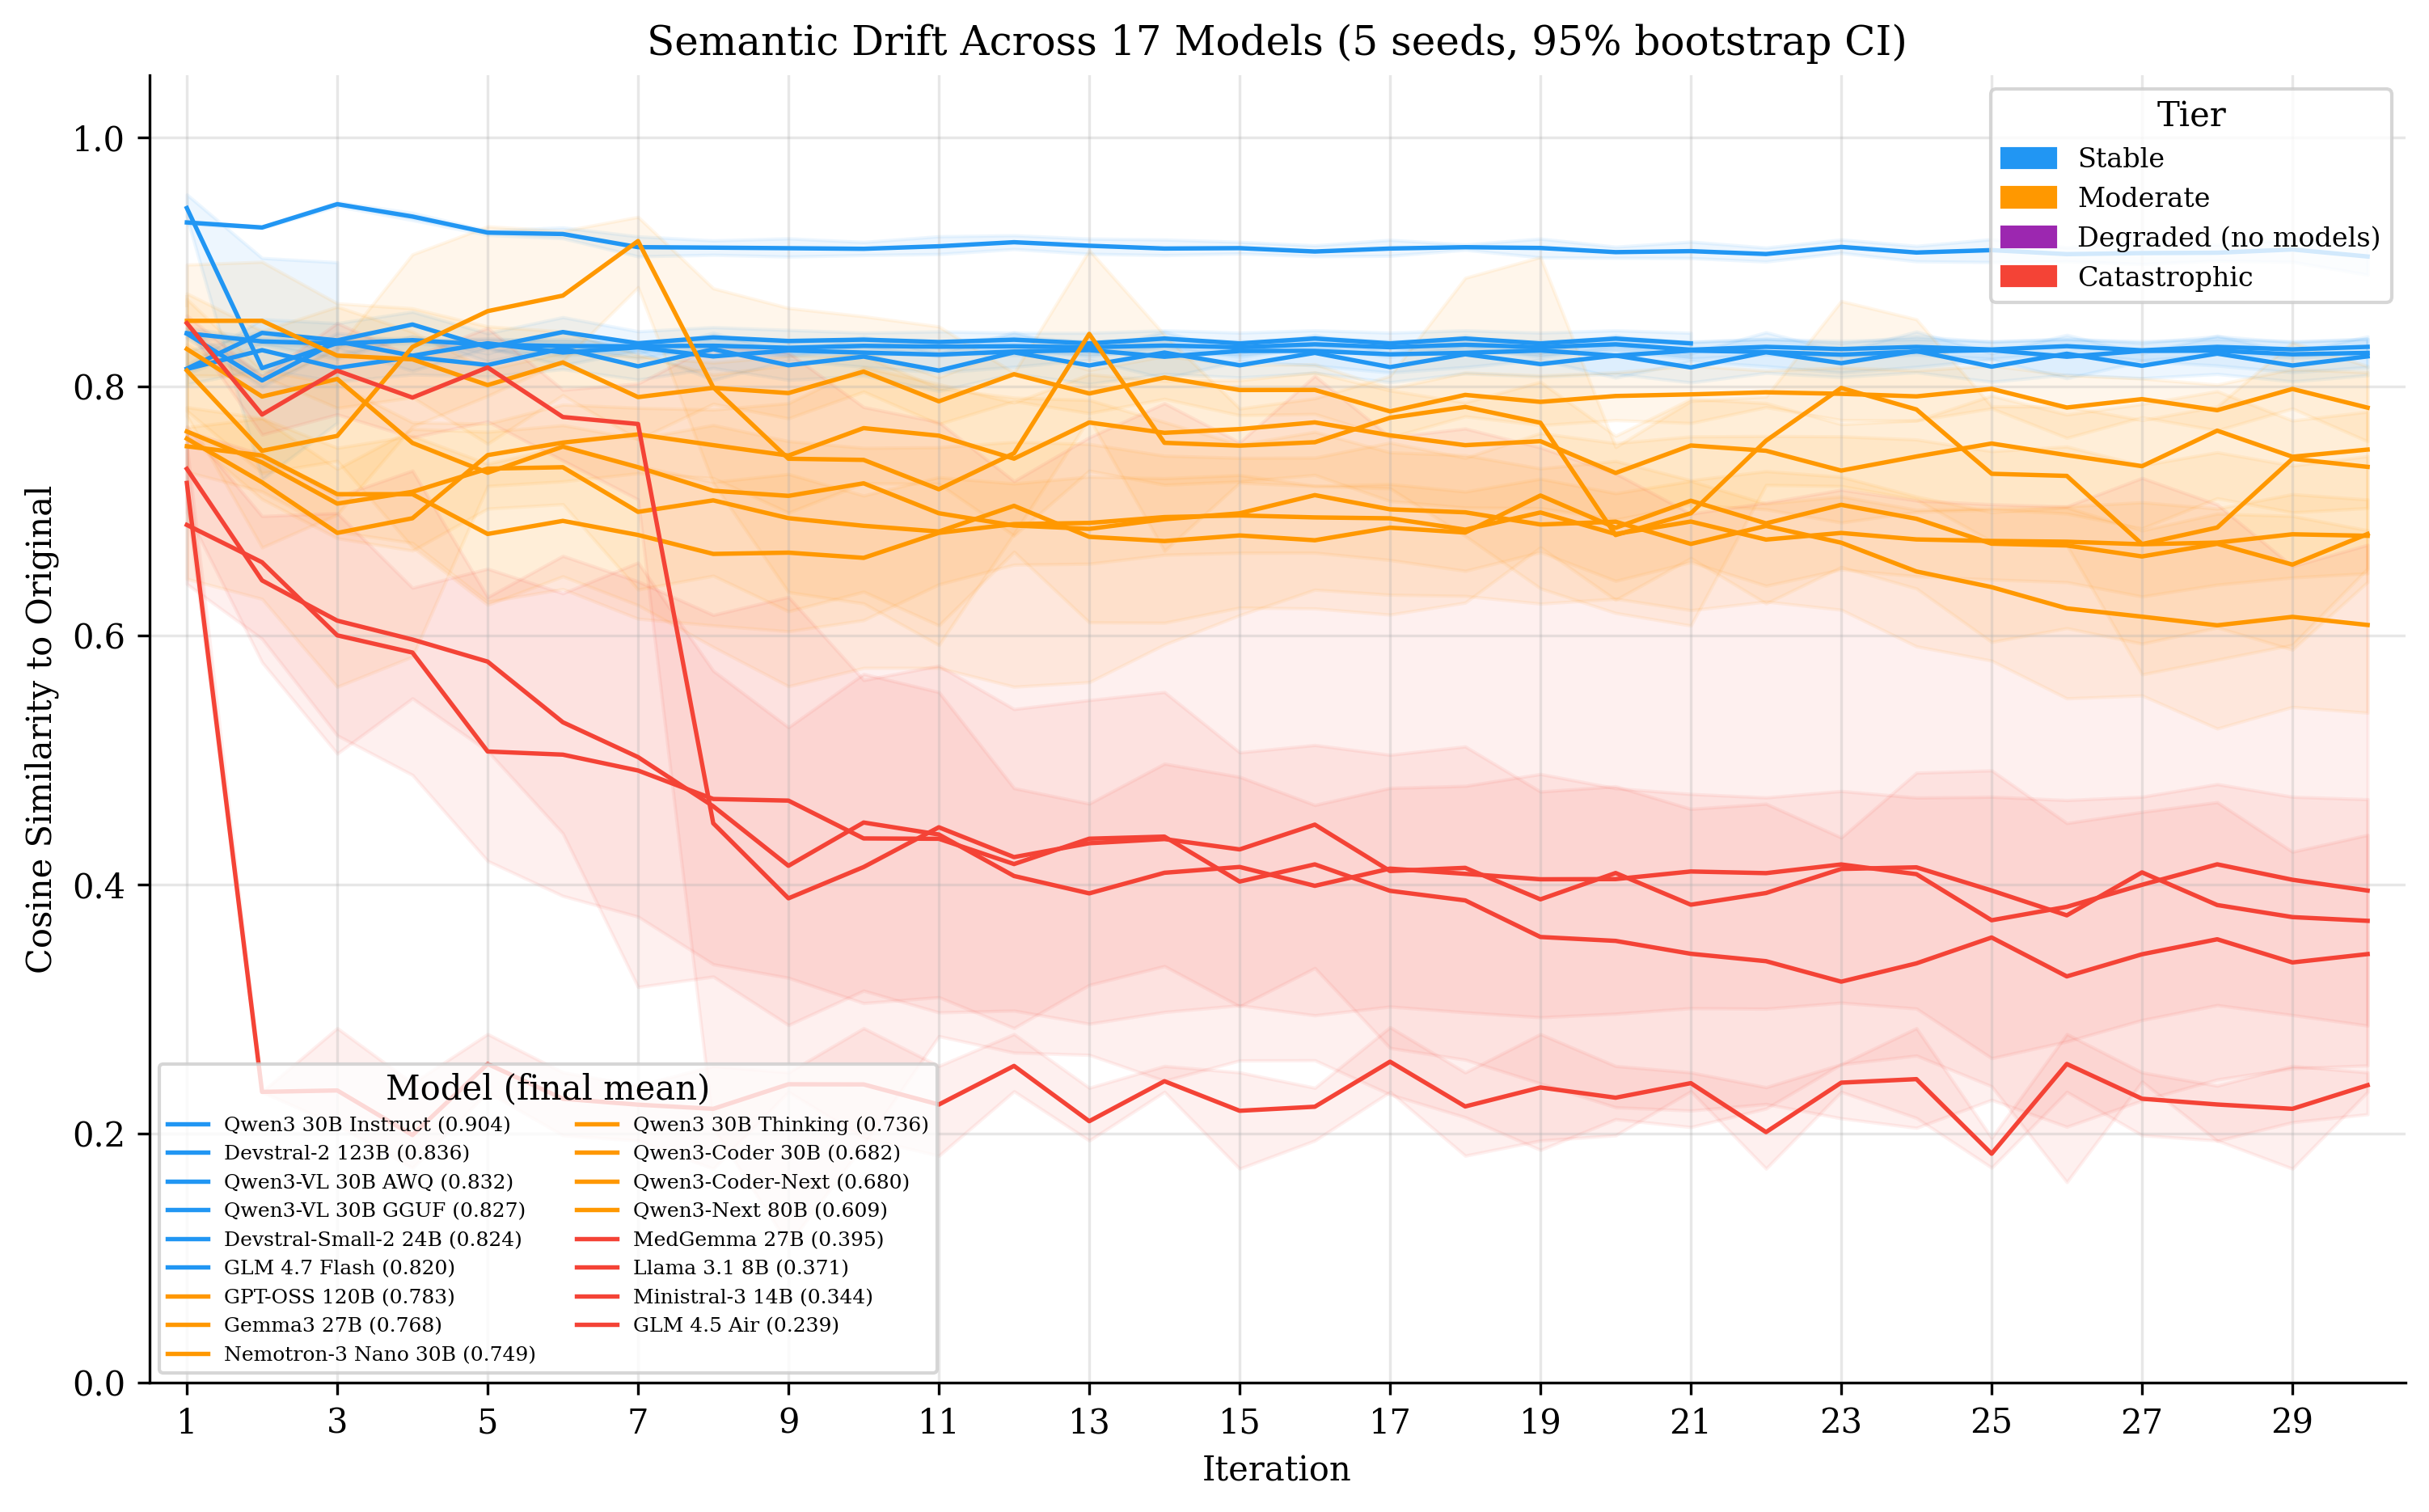
\includegraphics[width=\textwidth,height=0.31\textheight,keepaspectratio]{../results/paper_figures/fig1_rq1_lines.png}
  \caption{Semantic drift across 17 models. Lines show mean cosine similarity
  to the original across up to 5 seed-chains; shaded regions indicate 95\%
  bootstrap CI. Llama~3.1~8B and GLM~4.5~Air rest on $n=3$ (two chains each
  produced no scored iteration), and the GLM~4.7~Flash curves end early
  because all five of its chains terminated before iteration~30; see
  Table~\ref{tab:rq1}. The Degraded band (0.40--0.60) is empty in this
  study and is labelled as such in the legend.}
  \label{fig:rq1_lines}
\end{figure}

\begin{figure}[htbp]
  \centering
  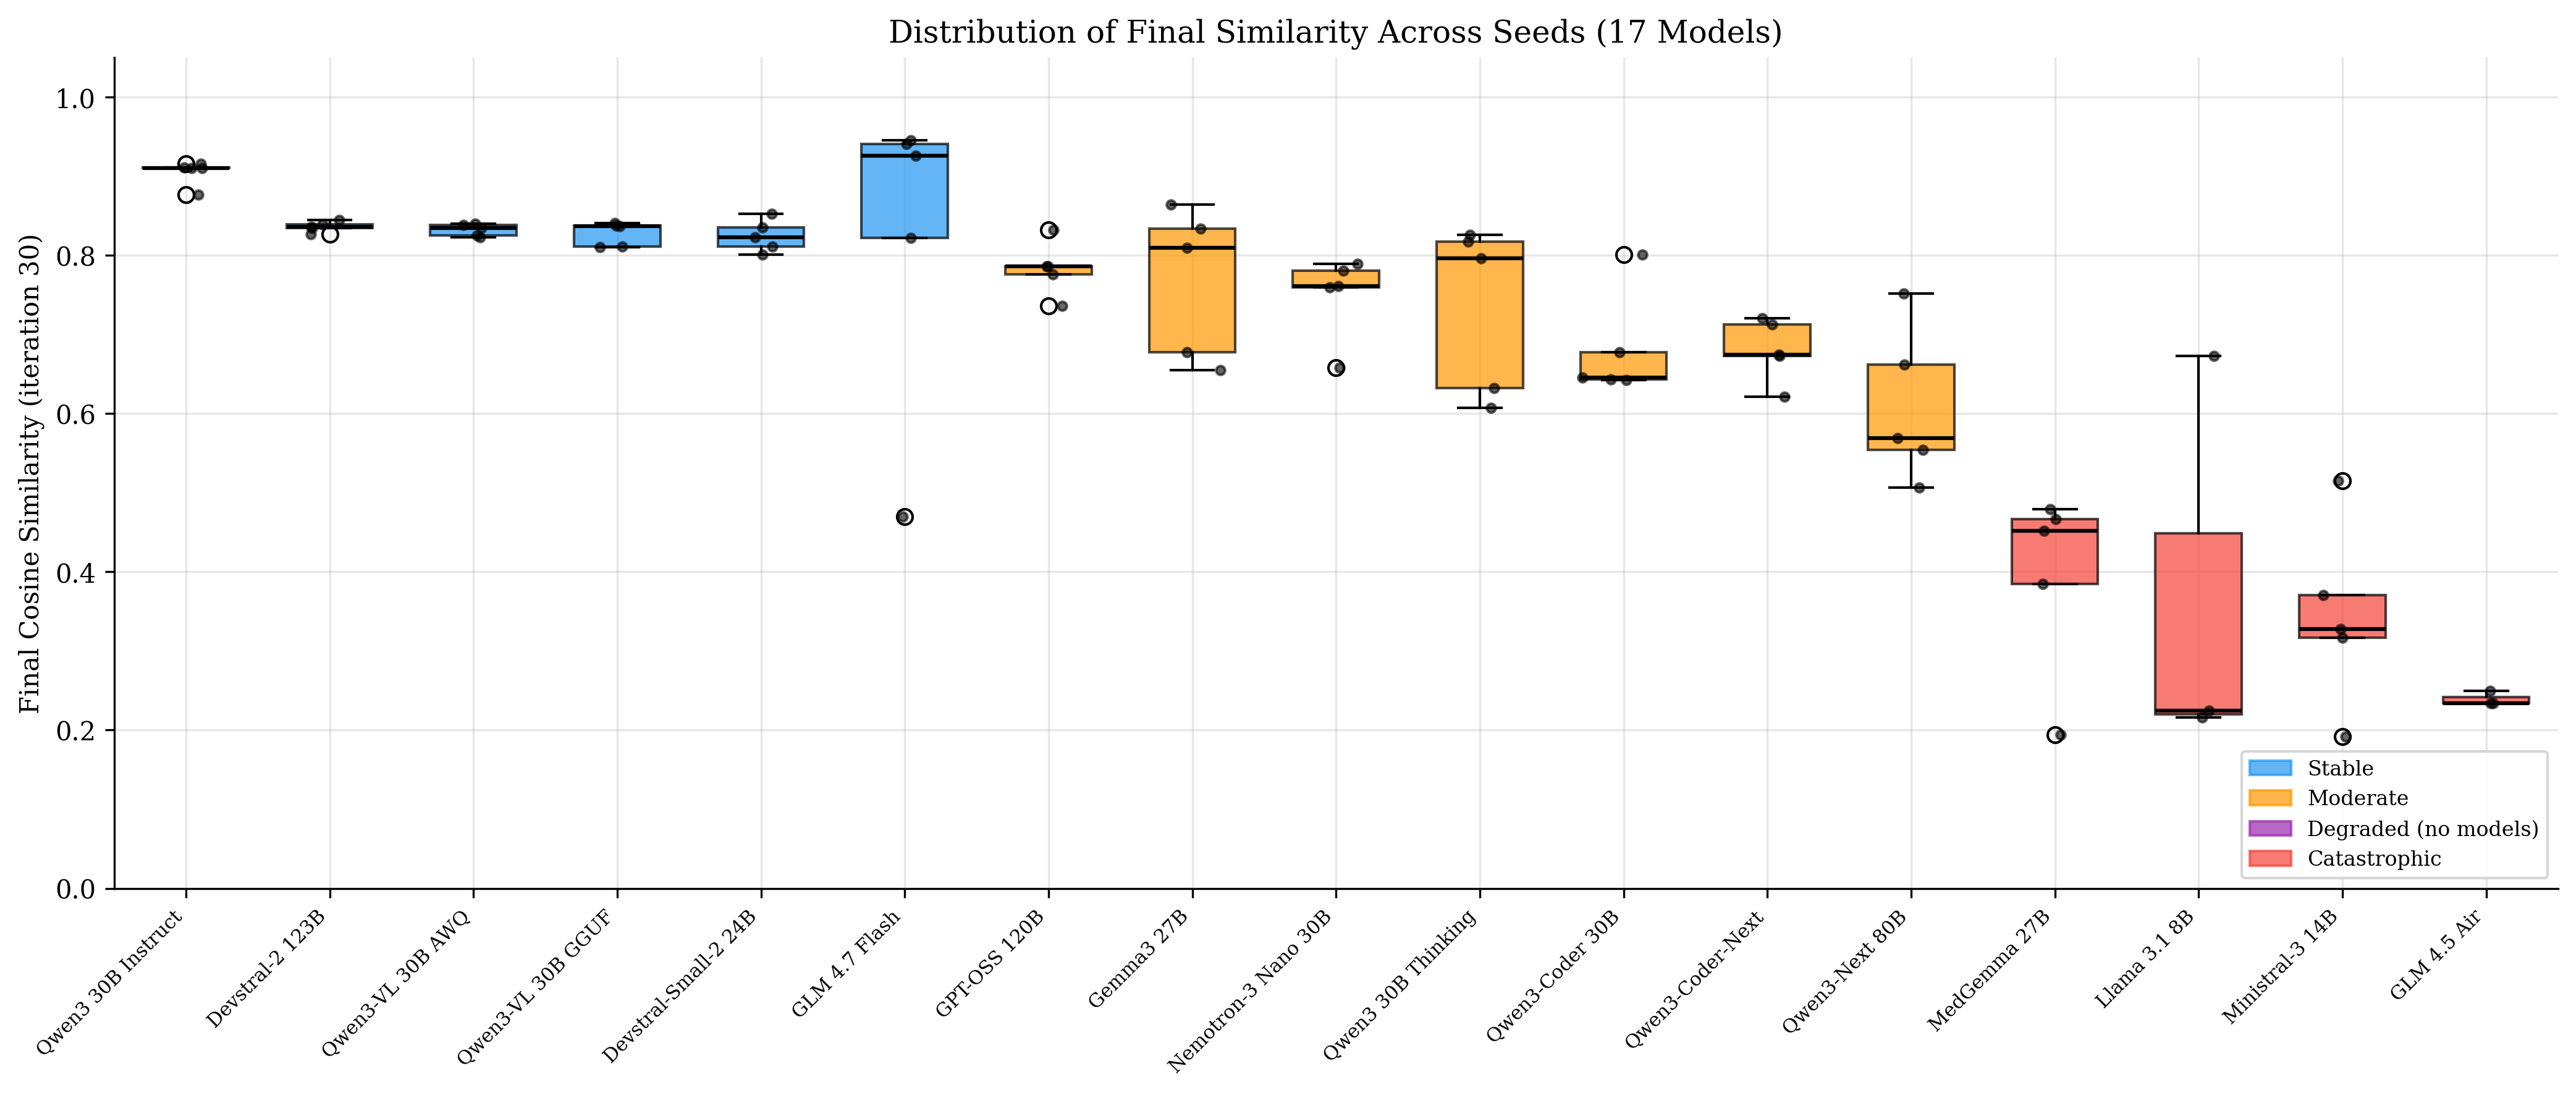
\includegraphics[width=\textwidth,height=0.31\textheight,keepaspectratio]{../results/paper_figures/fig2_rq1_boxplot.png}
  \caption{Distribution of final cosine similarity across the available
  seed-chains for each model (5 unless noted in Table~\ref{tab:rq1}; for a
  chain that terminated early the final value is its last scored iteration
  rather than iteration~30). Colors indicate stability tier; the Degraded
  band is empty in this study. Note the high variance in catastrophic-tier
  models.}
  \label{fig:rq1_boxplot}
\end{figure}

\begin{table}[t]
\centering
\caption{Per-model drift statistics (RQ1). Mean final cosine similarity
  with 95\% bootstrap CI, sorted by mean descending. Five chains were
  launched per model; $n$ is the number that returned at least one scored
  iteration and is the number the mean and CI are computed over, while
  $n_{30}$ is the number that ran the full 30 iterations. Rows with
  $n<5$ or $n_{30}<n$ are marked $\dagger$: the final similarity for a
  truncated chain is its last scored iteration, not iteration 30.}
\label{tab:rq1}
\small
\begin{tabular}{lccccl}
\toprule
Model & Mean & 95\% CI & $n$ & $n_{30}$ & Tier \\
\midrule
Qwen3 30B Instruct & 0.904 & [0.890, 0.913] & 5 & 5 & Stable \\
Devstral-2 123B & 0.836$^\dagger$ & [0.831, 0.841] & 5 & 4 & Stable \\
Qwen3-VL 30B AWQ & 0.832 & [0.826, 0.838] & 5 & 5 & Stable \\
Qwen3-VL 30B GGUF & 0.827 & [0.816, 0.839] & 5 & 5 & Stable \\
Devstral-Small-2 24B & 0.824 & [0.809, 0.840] & 5 & 5 & Stable \\
GLM 4.7 Flash & 0.820$^\dagger$ & [0.635, 0.939] & 5 & 0 & Stable \\
\midrule
GPT-OSS 120B & 0.783 & [0.756, 0.812] & 5 & 5 & Moderate \\
Gemma3 27B & 0.768$^\dagger$ & [0.695, 0.841] & 5 & 4 & Moderate \\
Nemotron-3 Nano 30B & 0.749 & [0.702, 0.780] & 5 & 5 & Moderate \\
Qwen3 30B Thinking & 0.736 & [0.654, 0.816] & 5 & 5 & Moderate \\
Qwen3-Coder 30B & 0.682 & [0.643, 0.744] & 5 & 5 & Moderate \\
Qwen3-Coder-Next & 0.680 & [0.650, 0.709] & 5 & 5 & Moderate \\
Qwen3-Next 80B & 0.609 & [0.538, 0.694] & 5 & 5 & Moderate \\
\midrule
MedGemma 27B & 0.395 & [0.289, 0.469] & 5 & 5 & Catastrophic \\
Llama 3.1 8B & 0.371$^\dagger$ & [0.216, 0.673] & 3 & 3 & Catastrophic \\
Ministral-3 14B & 0.344 & [0.255, 0.440] & 5 & 5 & Catastrophic \\
GLM 4.5 Air & 0.239$^\dagger$ & [0.234, 0.249] & 3 & 3 & Catastrophic \\
\bottomrule
\end{tabular}
\end{table}



\subsection{Within-Family Scaling and Quantization Level}
\label{sec:scaling}

Holding the architecture fixed removes the family confound that limits
Section~\ref{sec:rq1}. Figure~\ref{fig:q35_lines} shows drift trajectories for
all 18 Qwen3.5 GGUF configurations on the spaghetti recipe, and
Table~\ref{tab:size_quant} gives summary statistics for both recipes with the
$n$ behind each cell.

\begin{figure}[htbp]
\centering
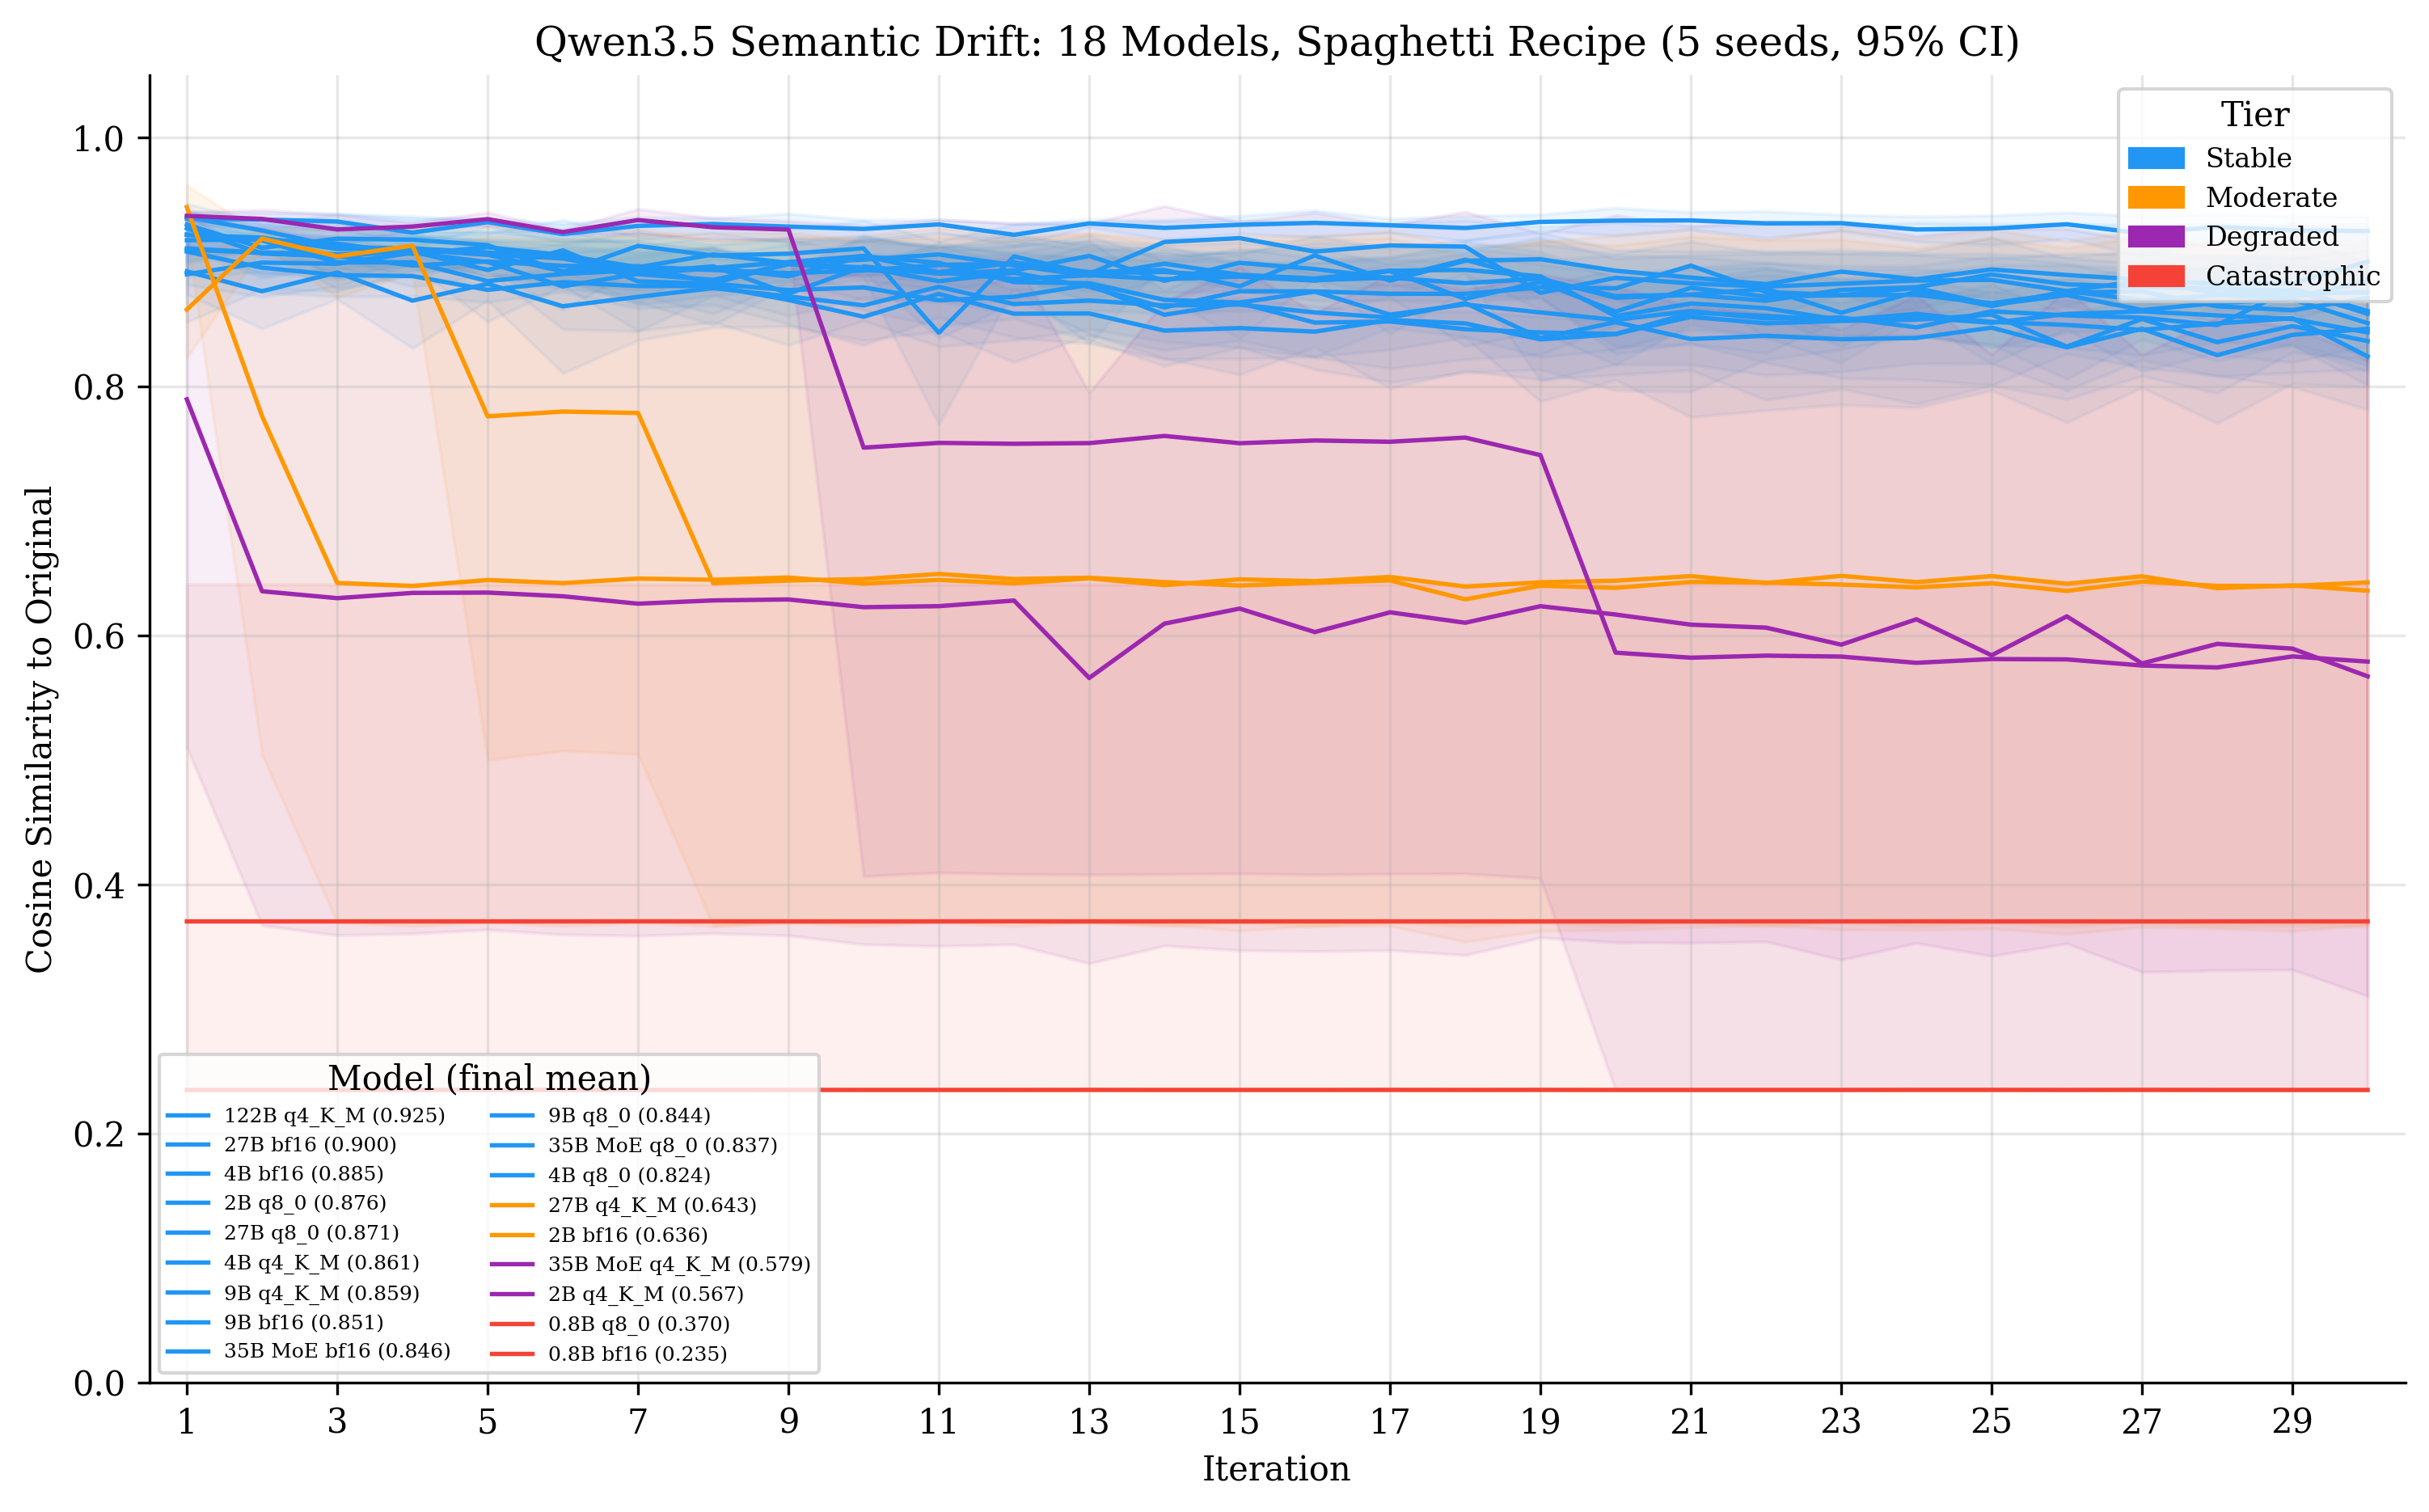
\includegraphics[width=\textwidth,height=0.31\textheight,keepaspectratio]{../results/qwen35_paper_figures/fig1_size_quant_lines.png}
\caption{Semantic drift across 18 Qwen3.5 GGUF models (spaghetti recipe,
  up to 5 completed chains per model, 95\% bootstrap CI bands). Models
  colored by stability tier; per-model $n$ is given in
  Table~\ref{tab:size_quant}.}
\label{fig:q35_lines}
\end{figure}

\begin{table}[t]
\centering
\caption{Qwen3.5 drift by size and quantization. Mean final cosine
  similarity at iteration 30 over \emph{clean} chains only (chains with
  no empty, runaway-thinking generation), with 95\% bootstrap CI,
  sorted by clean spaghetti mean descending. $n_c$ is the number of
  clean 30-iteration chains behind each mean; ``RA'' is the
  runaway-thinking rate, i.e.\ the fraction of completed chains that
  contained at least one empty generation (runaway chains are excluded
  from the means). All-chain means are reported in the supplementary
  \texttt{all\_stats.json}.}
\label{tab:size_quant}
\footnotesize
\resizebox{\textwidth}{!}{%
\begin{tabular}{llcccccccl}
\toprule
Size & Quant & \multicolumn{4}{c}{Spaghetti} & \multicolumn{3}{c}{Lasagna} & Tier \\
\cmidrule(lr){3-6}\cmidrule(lr){7-9}
 & & Mean & 95\% CI & $n_c$ & RA & Mean & $n_c$ & RA & \\
\midrule
122B & q4\_K\_M & 0.925 & [0.915, 0.937] & 5 & 0.00 (0/5) & 0.864 & 5 & 0.00 (0/5) & Stable \\
35B MoE & q4\_K\_M & 0.923 & [0.920, 0.927] & 2 & 0.50 (2/4) & 0.812 & 5 & 0.00 (0/5) & Stable \\
27B & q4\_K\_M & 0.914 & [0.898, 0.929] & 3 & 0.40 (2/5) & 0.829 & 5 & 0.00 (0/5) & Stable \\
0.8B & q8\_0 & 0.912 & [0.912, 0.912] & 1 & 0.80 (4/5) & --- & 0 & 1.00 (5/5) & Stable \\
2B & bf16 & 0.903 & [0.892, 0.926] & 3 & 0.40 (2/5) & 0.760 & 2 & 0.60 (3/5) & Stable \\
27B & bf16 & 0.900 & [0.886, 0.914] & 5 & 0.00 (0/5) & 0.855 & 5 & 0.00 (0/5) & Stable \\
4B & bf16 & 0.885 & [0.873, 0.899] & 5 & 0.00 (0/5) & 0.741 & 5 & 0.00 (0/5) & Stable \\
2B & q8\_0 & 0.876 & [0.814, 0.931] & 5 & 0.00 (0/5) & 0.846 & 1 & 0.80 (4/5) & Stable \\
27B & q8\_0 & 0.871 & [0.833, 0.910] & 5 & 0.00 (0/5) & 0.839 & 5 & 0.00 (0/5) & Stable \\
4B & q4\_K\_M & 0.861 & [0.819, 0.899] & 5 & 0.00 (0/5) & 0.823 & 5 & 0.00 (0/5) & Stable \\
9B & q4\_K\_M & 0.859 & [0.820, 0.892] & 5 & 0.00 (0/5) & 0.830 & 5 & 0.00 (0/5) & Stable \\
9B & bf16 & 0.851 & [0.811, 0.893] & 5 & 0.00 (0/5) & 0.815 & 5 & 0.00 (0/5) & Stable \\
35B MoE & bf16 & 0.846 & [0.798, 0.887] & 5 & 0.00 (0/5) & 0.797 & 5 & 0.00 (0/5) & Stable \\
9B & q8\_0 & 0.844 & [0.783, 0.893] & 5 & 0.00 (0/5) & 0.795 & 5 & 0.00 (0/5) & Stable \\
35B MoE & q8\_0 & 0.837 & [0.815, 0.858] & 5 & 0.00 (0/5) & 0.803 & 5 & 0.00 (0/5) & Stable \\
4B & q8\_0 & 0.824 & [0.801, 0.846] & 5 & 0.00 (0/5) & 0.788 & 5 & 0.00 (0/5) & Stable \\
\midrule
2B & q4\_K\_M & 0.789 & [0.612, 0.889] & 3 & 0.40 (2/5) & 0.772 & 4 & 0.20 (1/5) & Moderate \\
\midrule
0.8B & bf16 & --- & --- & 0 & 1.00 (5/5) & --- & 0 & 1.00 (5/5) & Catastrophic \\
\bottomrule
\end{tabular}}
\end{table}


\paragraph{Stability threshold at 4B.}
Table~\ref{tab:size_quant} reports two statistics per cell: the mean over
\emph{clean} chains, those that produced text at every iteration, and the
rate at which chains instead entered the runaway-thinking failure mode of
Section~\ref{sec:runaway}, after which every remaining iteration is empty and
similarity sits at the embedding floor (0.235 for spaghetti, 0.064 for
lasagna). Among clean chains, every configuration at or above 4B parameters
reaches a mean final similarity between 0.82 and 0.93 on spaghetti, and
between 0.74 and 0.86 on lasagna. Below 4B the picture changes in kind
rather than degree. The 0.8B models produce no clean lasagna chain at all
and only one clean spaghetti chain in ten; the 2B models lose 20--80\% of
their chains to runaway depending on precision and recipe. A model below the
threshold is therefore not merely a noisier paraphraser but one whose
chains fail outright in a large fraction of runs.

\paragraph{Non-monotonic precision.}
Within the clean chains, precision level does not order drift. For the 4B
dense model BF16 (0.885) leads Q4\_K\_M (0.861) and Q8\_0 (0.824). For the
27B dense model the order is Q4\_K\_M (0.914, $n=3$), BF16 (0.900), Q8\_0
(0.871), and for the 35B MoE it is Q4\_K\_M (0.923, $n=2$), BF16 (0.846),
Q8\_0 (0.837). For the 2B model BF16 (0.903, $n=3$) edges Q8\_0 (0.876) on
spaghetti, but on lasagna Q8\_0 loses four of five chains to runaway while
Q4\_K\_M loses one. Higher precision therefore does not guarantee less
drift---the conclusion the KV-cache experiment reaches by another route
(Section~\ref{sec:rq2})---but the comparison must be read together with the
failure rates: at 4-bit the clean means are the highest in their size class
and rest on the fewest chains, because 40--50\% of the 27B and 35B Q4\_K\_M
spaghetti chains ran away. When every completed chain is counted instead,
those two cells fall to 0.643 and 0.579 (Table~\ref{tab:size_quant},
``all'' arm in the released statistics), and the apparent precision penalty
is entirely a failure-rate penalty.

\paragraph{Mixture-of-experts and the largest model.}
The 122B MoE achieves the family's best spaghetti score (0.925, CI
[0.915, 0.937]) with no runaway chains at any precision, and its lasagna
score (0.864) is also the family's best. At matched parameter counts the
35B MoE and the 27B dense model are indistinguishable on clean chains
(0.837--0.923 vs.\ 0.871--0.914 across precisions) and share the same
Q4\_K\_M runaway rate; the sparse-activation advantage suggested by the
cross-family tiers is not reproduced within the family.

\paragraph{Statistical tests.}
Assigning each configuration to a tier by its all-chain spaghetti mean
occupies all four tiers (12 Stable, 2 Moderate, 2 Degraded, 2
Catastrophic). Kruskal--Wallis across the occupied tiers gives $H = 18.19$,
$p = 4.0 \times 10^{-4}$, with Cohen's $d = 6.18$ between Stable and
Catastrophic and $1.67$ between Stable and Moderate, subject to the
independence caveat of Section~\ref{sec:stats}. Because the Moderate and
Degraded tiers are populated only by the runaway-affected Q4\_K\_M and 2B
cells, the tier structure within the family is largely a failure-rate
structure.

\paragraph{Interaction with stimulus complexity.}
Figure~\ref{fig:q35_heatmap} presents the size $\times$ precision heatmap
for both recipes, and Figure~\ref{fig:q35_complexity} contrasts them across
all 18 configurations. For models above the threshold the lasagna mean is
consistently the lower of the two, by 0.03--0.14 (122B: 0.925 vs.\ 0.864;
27B BF16: 0.900 vs.\ 0.855; 4B BF16: 0.885 vs.\ 0.741), the expected
cost of carrying a 21-step context through 30 rewrites. The runaway failure
mode has the opposite dependence: on the 27B and 35B Q4\_K\_M builds it
occurs only on the 3-step spaghetti stimulus and never on lasagna, and on the
35B NVFP4 build (Section~\ref{sec:quantformat}) the spaghetti rate is 80\%
against 0\% on lasagna. Short inputs, not long ones, trigger runaway
thinking; the most plausible reading is that a trivial rewriting task gives
the model's reasoning process no natural stopping point.

\begin{figure}[htbp]
\centering
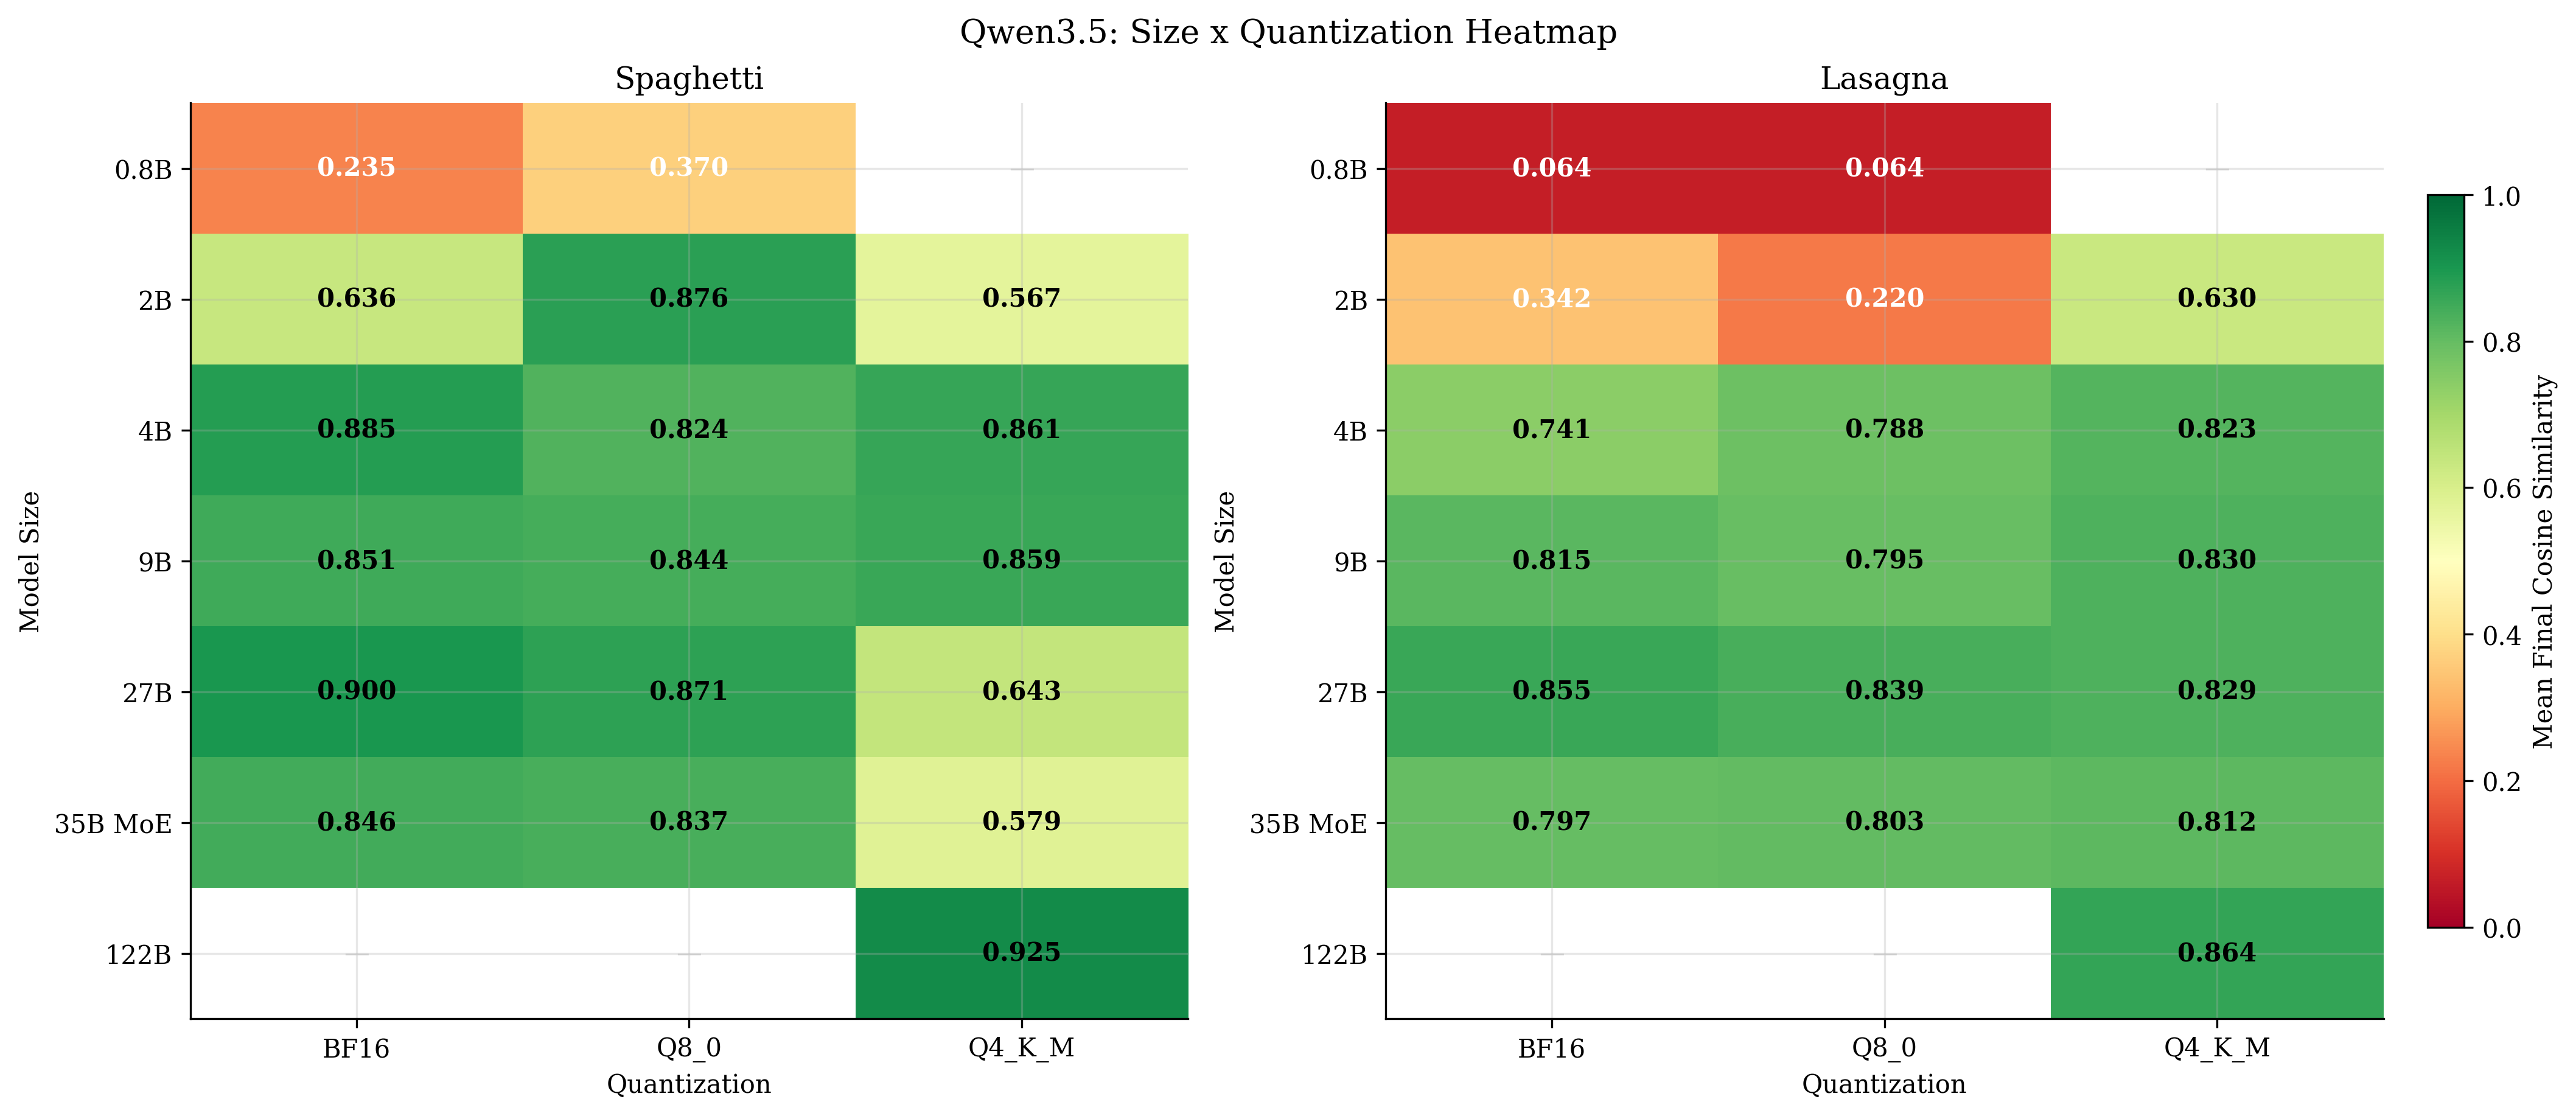
\includegraphics[width=\textwidth,height=0.31\textheight,keepaspectratio]{../results/qwen35_paper_figures/fig3_quant_heatmap.png}
\caption{Mean final similarity by model size and quantization level.
  Left: spaghetti recipe. Right: lasagna recipe.
  Note that 0.8B Q4\_K\_M does not exist for Qwen3.5.}
\label{fig:q35_heatmap}
\end{figure}

\begin{figure}[htbp]
\centering
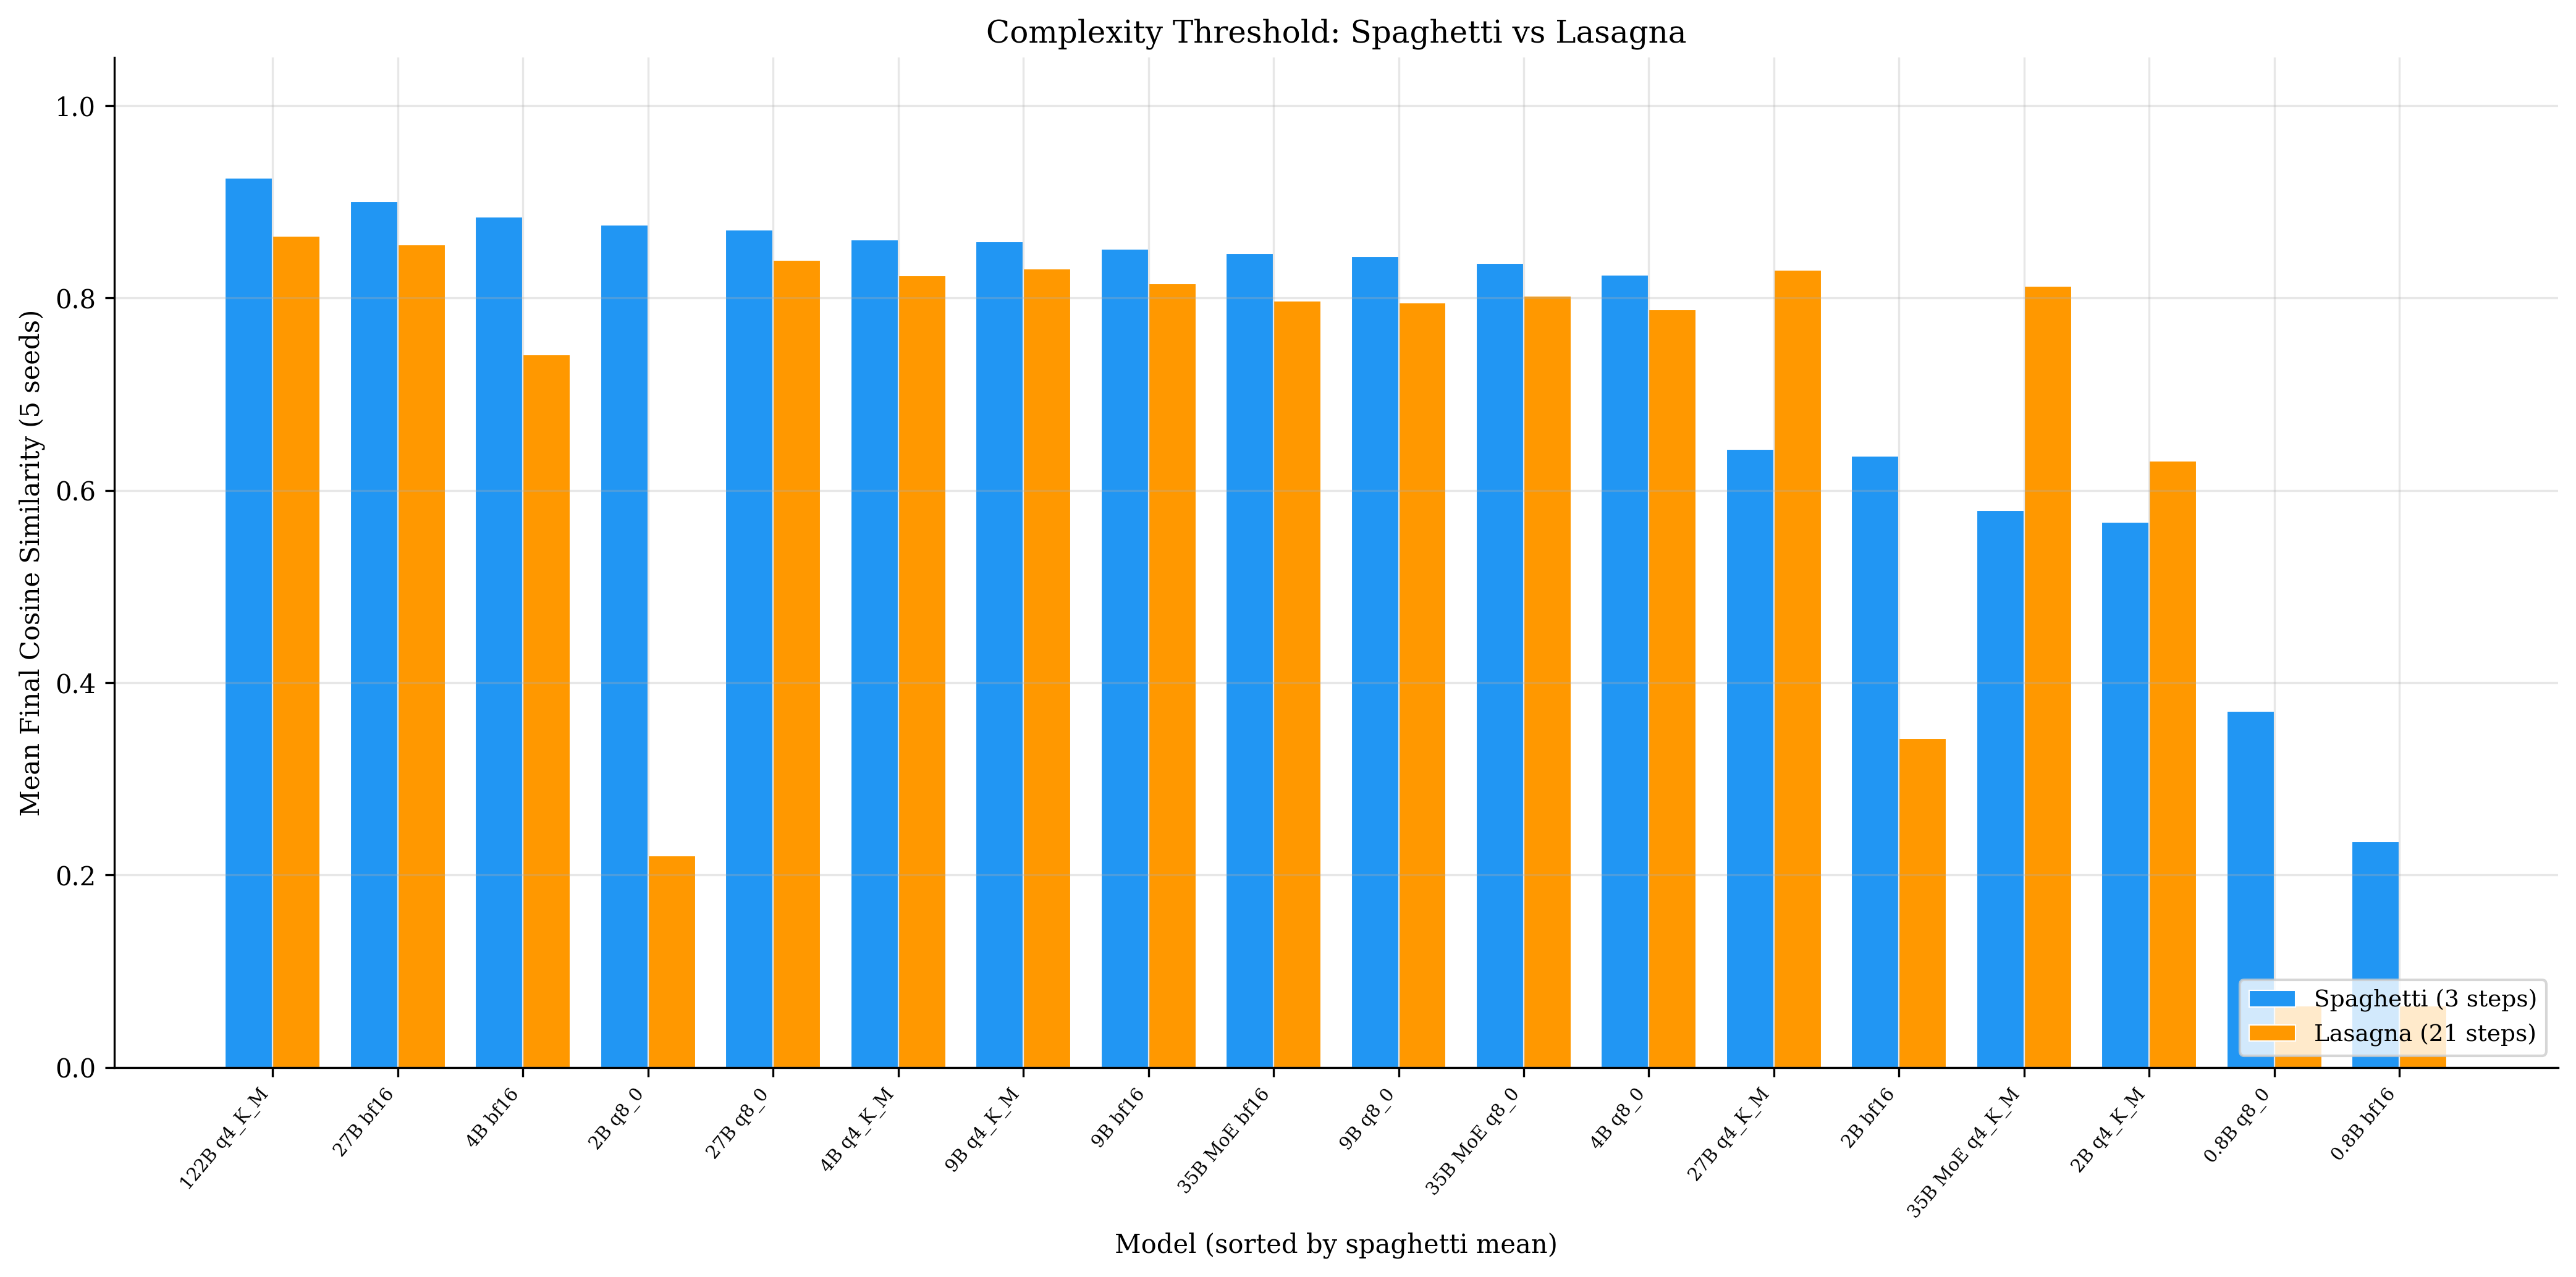
\includegraphics[width=\textwidth,height=0.31\textheight,keepaspectratio]{../results/qwen35_paper_figures/fig6_complexity_threshold.png}
\caption{Spaghetti (3 steps) vs.\ lasagna (21 steps) for all Qwen3.5
  GGUF models. Solid bars: spaghetti. Hatched bars: lasagna.}
\label{fig:q35_complexity}
\end{figure}


\clearpage
\subsection{Runaway Thinking as a Failure Mode}
\label{sec:runaway}

Drift within these chains is not always gradual. A substantial minority of
within-family chains fail discretely: the model returns an empty completion,
the chain re-feeds the same input at the next iteration, and every subsequent
completion is empty as well. Table~\ref{tab:runaway}, Table~\ref{tab:runaway_prompts} and
Figure~\ref{fig:runaway} report the rate at which each condition does so.

\paragraph{What an empty completion is.}
The empties are not serving errors. Every one is a successful API response
whose generation ran for the full 16{,}384-token budget: on each model the
wall time of an empty iteration is constant to within a second and equals the
budget divided by that model's measured decode rate (303\,s on the 27B GGUF
build at 54 tokens/s, 116\,s on the 35B MoE GGUF build at 141 tokens/s,
120--260\,s on the 35B NVFP4 build). Qwen3.5 enables reasoning by default,
and both Ollama and SGLang strip the reasoning block from the returned
content. An empty completion is therefore a generation that never left the
thinking block: the model reasoned until the budget was exhausted and emitted
no answer. We call this \emph{runaway thinking}. The Qwen3.5 embedding
appendix (Appendix~\ref{app:embedding}) documents the complementary
failure at the other extreme, chains whose outputs grow past 6{,}000 words;
that mode is rare in the baseline conditions and is driven by specific
system prompts, so this section concentrates on the empty-completion mode.

\paragraph{Rates.}
Across the 1{,}969 completed within-family chains, 265 (13.5\%, Wilson 95\%
CI [12.0\%, 15.0\%]) are runaway. The rate is governed first by the serving
stack: it is zero across all 993 chains served by vLLM (35B AWQ, 35B GPTQ-Int4,
9B AWQ; 743 chains) or by SGLang for the Nemotron control (250 chains), and
15--54\% on
the Ollama GGUF and SGLang NVFP4 arms. Within the Ollama sweep it then
follows size and precision (Table~\ref{tab:runaway}): both 0.8B builds fail
in 80--100\% of chains on either recipe; the 2B builds fail in 20--80\%; and
above 4B only the Q4\_K\_M builds fail, at 40\% (27B) and 50\% (35B MoE) on
spaghetti and never on lasagna. The 35B NVFP4 build on SGLang fails in 80\%
of baseline spaghetti chains and 0\% of lasagna chains. Onset is early: the
median first empty completion is at iteration 3 (mean 5.7), so a runaway
chain typically contributes only a handful of paraphrases before locking.

\paragraph{System prompts trigger it.}
The system-prompt sweep (Section~\ref{sec:rq3}) shows that the prompt is as
strong a trigger as the model. On the 35B NVFP4 build, ten of the twenty
prompts produce runaway in every spaghetti chain and two---Strong Anti-Meta
and Ultra-Constrained Fidelity---in every lasagna chain, lifting that
configuration's overall rate to 54\%. Ultra-Constrained Fidelity and 100\% Fidelity raise the 27B GGUF spaghetti
rate to 80\%, and Ultra-Constrained Fidelity does the same on the 9B GGUF
lasagna set, a build that runs away in only 5\% of chains
otherwise. The prompts that trigger runaway are the ones that most tightly
constrain the output format or forbid commentary; an instruction that leaves
the model little to say appears to leave its reasoning process with no way
to conclude. On the vLLM arms, where reasoning is disabled by the serving
configuration, the same prompts produce no empties at all.

\paragraph{Consequence for every other statistic.}
Because a runaway chain sits at the embedding floor from its onset, a mean
over all completed chains mixes a fidelity measurement with a failure rate.
Every table in this paper therefore reports the clean-chain mean as the
primary statistic with the runaway rate beside it; the all-chain means are
retained in the released statistics. The two views can disagree sharply on
the same cell---0.923 clean against 0.579 all for the 35B Q4\_K\_M
spaghetti condition---and a reader interested in deployment risk should
weigh the rate at least as heavily as the mean.

\IfFileExists{../results/qwen35_paper_figures/fig11_runaway_rates.png}{%
\begin{figure}[htbp]
\centering
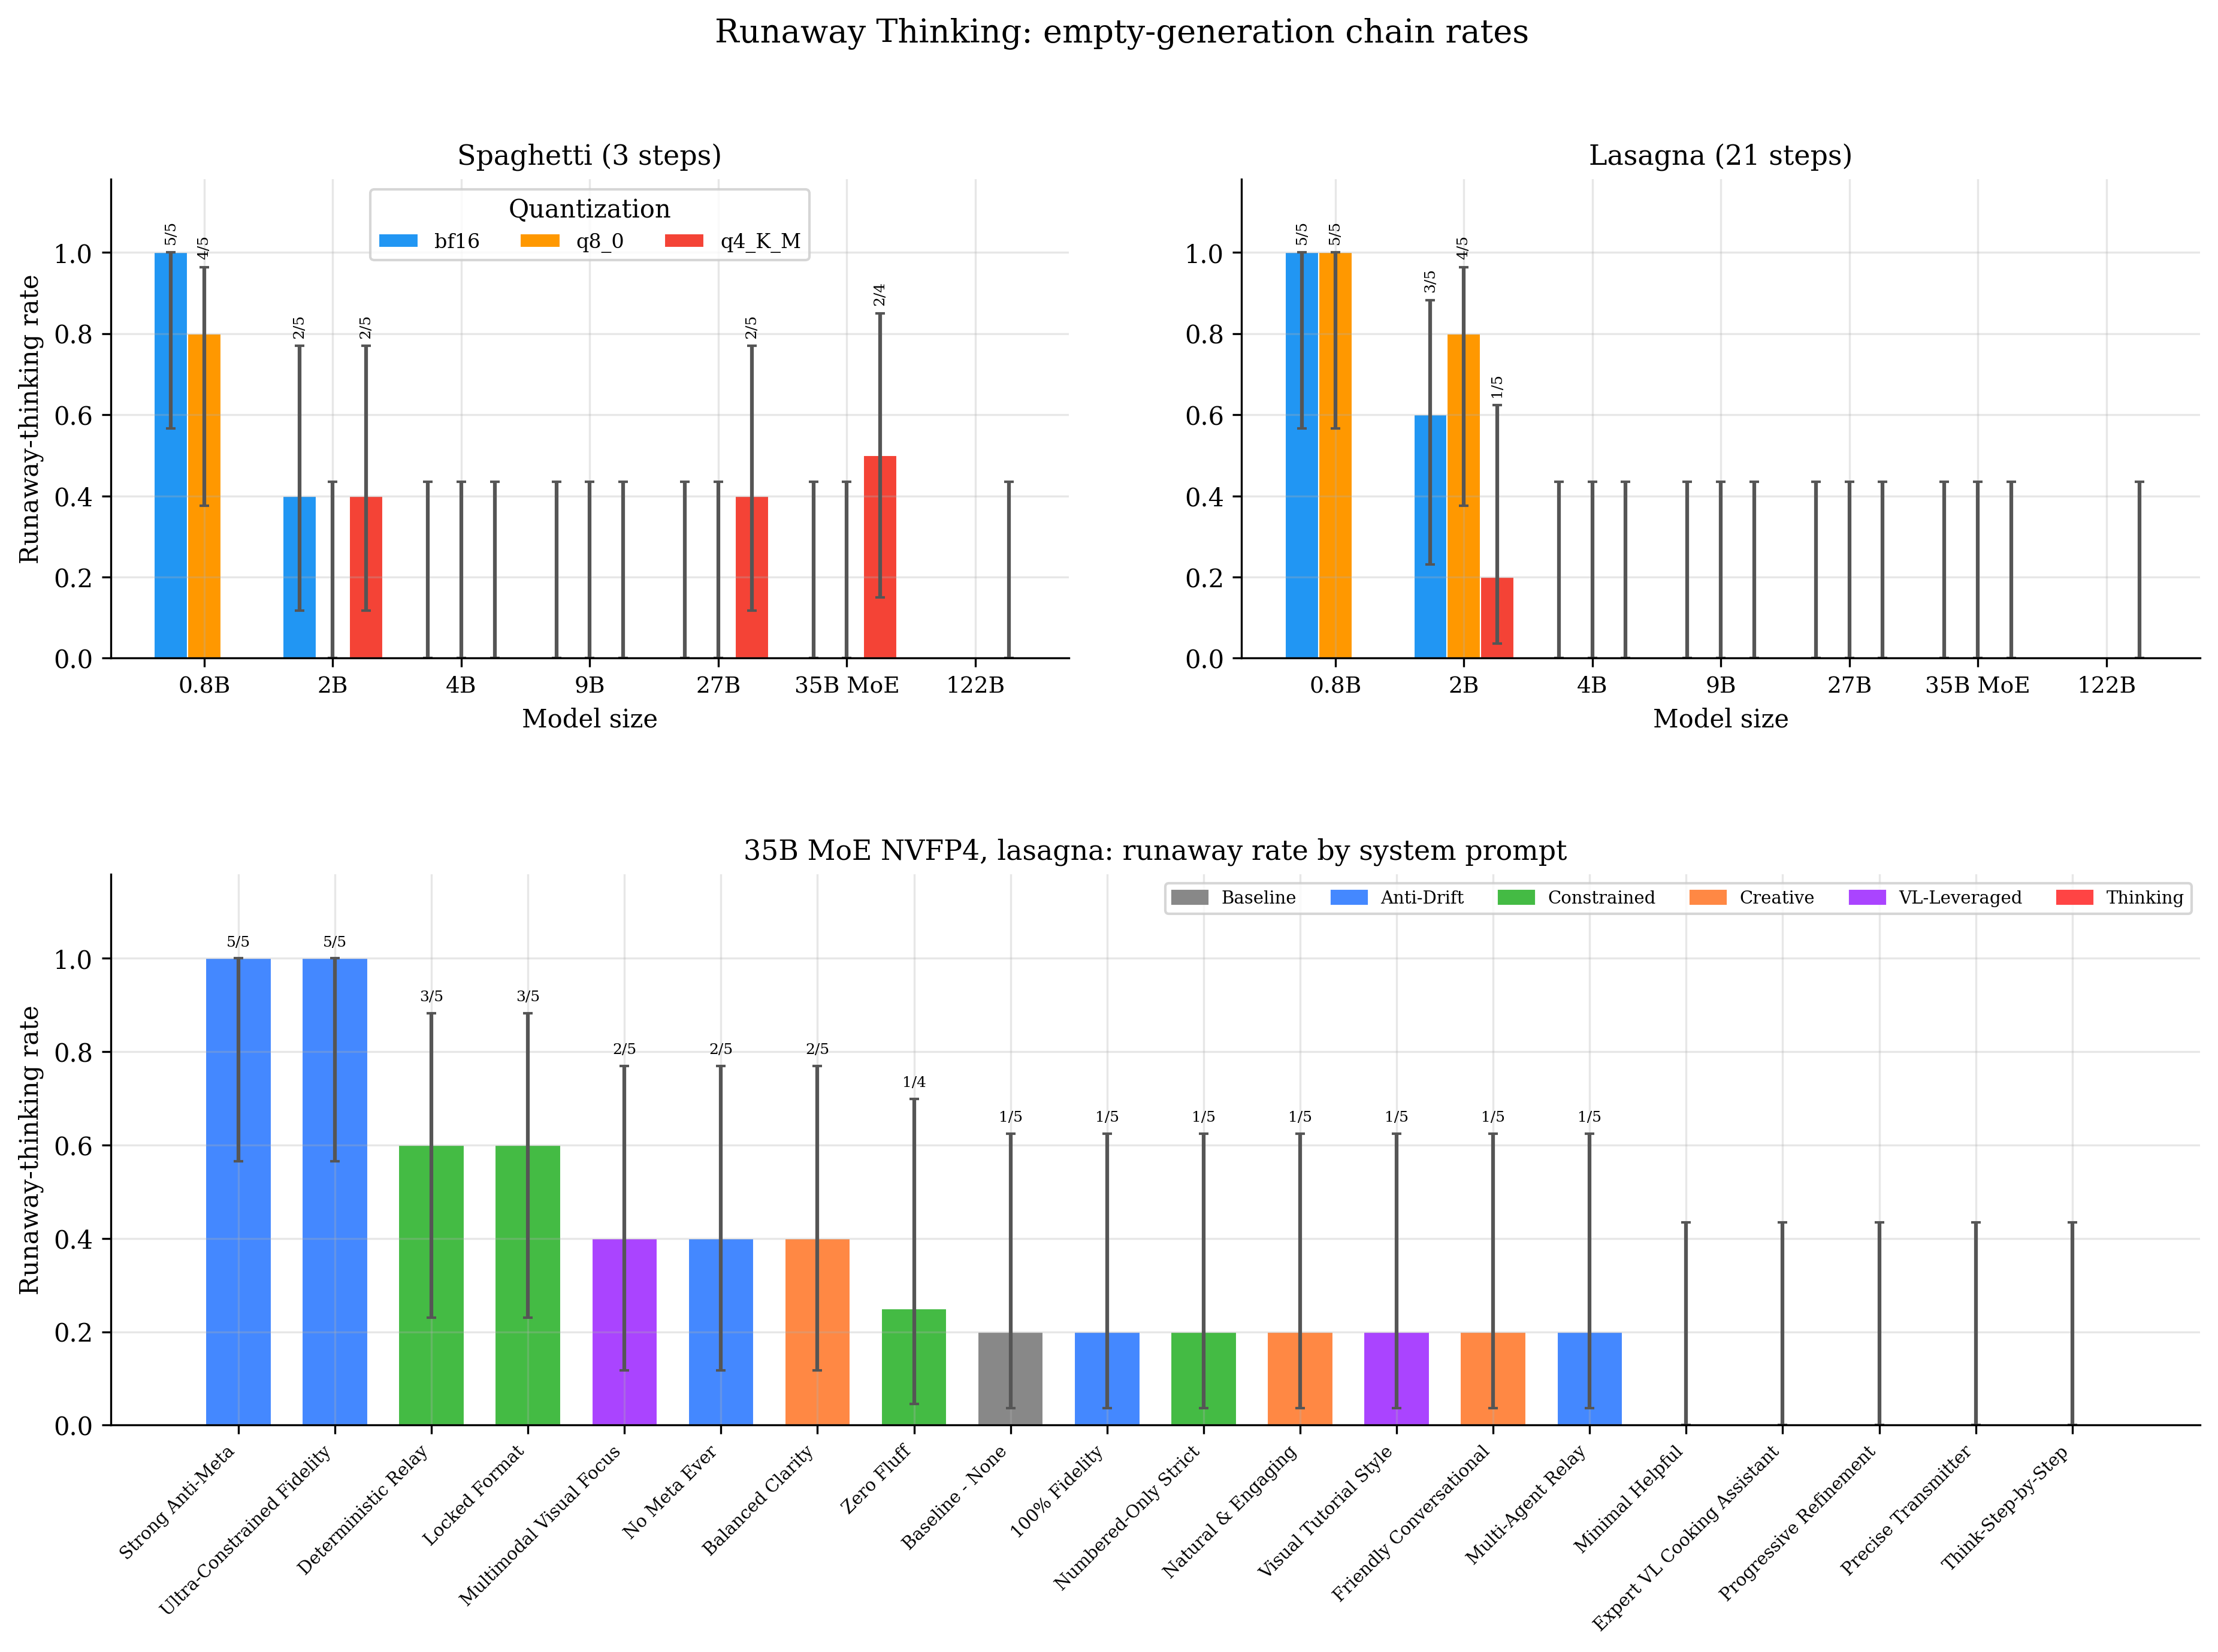
\includegraphics[width=\textwidth,height=0.31\textheight,keepaspectratio]{../results/qwen35_paper_figures/fig11_runaway_rates.png}
\caption{Runaway-generation rates by condition.}
\label{fig:runaway}
\end{figure}}{%
\begin{figure}[htbp]
\centering
\fbox{\parbox{0.9\textwidth}{\centering\vspace{2em}
\textit{fig11\_runaway\_rates.png not yet generated}\vspace{2em}}}
\caption{Runaway-generation rates by condition.}
\label{fig:runaway}
\end{figure}}

\IfFileExists{tables/table4_runaway.tex}{\begin{table}[p]
\centering
\caption{Runaway-thinking rates. A chain is \emph{runaway} when at
  least one of its 30 iterations returned an empty assistant message
  after a full-length generation, i.e.\ the entire token budget was
  consumed by reasoning; such chains never recover, because the same
  input is re-fed at the next iteration. Rate = runaway chains /
  completed chains, with a Wilson 95\% interval. Top block: RQ1 size
  $\times$ quantization set; per-prompt rates are in Table~\ref{tab:runaway_prompts}.}
\label{tab:runaway}
\footnotesize
\begin{tabular}{llcccc}
\toprule
Size & Quant & \multicolumn{2}{c}{Spaghetti} & \multicolumn{2}{c}{Lasagna} \\
\cmidrule(lr){3-4}\cmidrule(lr){5-6}
 & & Rate & 95\% CI & Rate & 95\% CI \\
\midrule
0.8B & q8\_0 & 0.80 (4/5) & [0.38, 0.96] & 1.00 (5/5) & [0.57, 1.00] \\
0.8B & bf16 & 1.00 (5/5) & [0.57, 1.00] & 1.00 (5/5) & [0.57, 1.00] \\
2B & q4\_K\_M & 0.40 (2/5) & [0.12, 0.77] & 0.20 (1/5) & [0.04, 0.62] \\
2B & q8\_0 & 0.00 (0/5) & [0.00, 0.43] & 0.80 (4/5) & [0.38, 0.96] \\
2B & bf16 & 0.40 (2/5) & [0.12, 0.77] & 0.60 (3/5) & [0.23, 0.88] \\
4B & q4\_K\_M & 0.00 (0/5) & [0.00, 0.43] & 0.00 (0/5) & [0.00, 0.43] \\
4B & q8\_0 & 0.00 (0/5) & [0.00, 0.43] & 0.00 (0/5) & [0.00, 0.43] \\
4B & bf16 & 0.00 (0/5) & [0.00, 0.43] & 0.00 (0/5) & [0.00, 0.43] \\
9B & q4\_K\_M & 0.00 (0/5) & [0.00, 0.43] & 0.00 (0/5) & [0.00, 0.43] \\
9B & q8\_0 & 0.00 (0/5) & [0.00, 0.43] & 0.00 (0/5) & [0.00, 0.43] \\
9B & bf16 & 0.00 (0/5) & [0.00, 0.43] & 0.00 (0/5) & [0.00, 0.43] \\
27B & q4\_K\_M & 0.40 (2/5) & [0.12, 0.77] & 0.00 (0/5) & [0.00, 0.43] \\
27B & q8\_0 & 0.00 (0/5) & [0.00, 0.43] & 0.00 (0/5) & [0.00, 0.43] \\
27B & bf16 & 0.00 (0/5) & [0.00, 0.43] & 0.00 (0/5) & [0.00, 0.43] \\
35B MoE & q4\_K\_M & 0.50 (2/4) & [0.15, 0.85] & 0.00 (0/5) & [0.00, 0.43] \\
35B MoE & q8\_0 & 0.00 (0/5) & [0.00, 0.43] & 0.00 (0/5) & [0.00, 0.43] \\
35B MoE & bf16 & 0.00 (0/5) & [0.00, 0.43] & 0.00 (0/5) & [0.00, 0.43] \\
122B & q4\_K\_M & 0.00 (0/5) & [0.00, 0.43] & 0.00 (0/5) & [0.00, 0.43] \\
\bottomrule
\end{tabular}

\end{table}

\begin{table}[p]
\centering
\caption{Runaway-thinking rate per system prompt (up to 5 chains per
  cell; rate = runaway chains / completed chains).}
\label{tab:runaway_prompts}
\footnotesize
\resizebox{\textwidth}{!}{%
\begin{tabular}{lcccc}
\toprule
System prompt & \multicolumn{2}{c}{35B MoE NVFP4} & \multicolumn{2}{c}{27B GGUF Q4\_K\_M} \\
\cmidrule(lr){2-3}\cmidrule(lr){4-5}
Prompt & Spag. & Las. & Spag. & Las. \\
\midrule
Baseline - None & 0.80 (4/5) & 0.20 (1/5) & 0.60 (3/5) & 0.00 (0/5) \\
Minimal Helpful & 0.60 (3/5) & 0.00 (0/5) & 0.20 (1/5) & 0.00 (0/5) \\
Strong Anti-Meta & 1.00 (5/5) & 1.00 (5/5) & 0.40 (2/5) & 0.40 (2/5) \\
Ultra-Constrained Fidelity & 1.00 (5/5) & 1.00 (5/5) & 0.80 (4/5) & 0.60 (3/5) \\
Expert VL Cooking Assistant & 0.60 (3/5) & 0.00 (0/5) & 0.20 (1/5) & 0.20 (1/5) \\
Deterministic Relay & 0.00 (0/5) & 0.60 (3/5) & 0.40 (2/5) & 0.40 (2/5) \\
100\% Fidelity & 1.00 (5/5) & 0.20 (1/5) & 0.80 (4/5) & 0.60 (3/5) \\
Numbered-Only Strict & 1.00 (5/5) & 0.20 (1/5) & 0.80 (4/5) & 0.00 (0/5) \\
Natural \& Engaging & 1.00 (5/5) & 0.20 (1/5) & 0.40 (2/5) & 0.20 (1/5) \\
Progressive Refinement & 1.00 (5/5) & 0.00 (0/5) & 0.40 (2/5) & 0.00 (0/5) \\
Visual Tutorial Style & 0.40 (2/5) & 0.20 (1/5) & 0.00 (0/5) & 0.20 (1/5) \\
Precise Transmitter & 0.60 (3/5) & 0.00 (0/5) & 0.00 (0/5) & 0.00 (0/5) \\
Zero Fluff & 1.00 (5/5) & 0.25 (1/4) & 0.20 (1/5) & 0.40 (2/5) \\
Locked Format & 1.00 (5/5) & 0.60 (3/5) & 0.60 (3/5) & 0.20 (1/5) \\
Friendly Conversational & 0.20 (1/5) & 0.20 (1/5) & 0.20 (1/5) & 0.00 (0/1) \\
Multi-Agent Relay & 0.80 (4/5) & 0.20 (1/5) & 0.00 (0/5) & 0.00 (0/3) \\
Think-Step-by-Step & 1.00 (5/5) & 0.00 (0/5) & 0.40 (2/5) & 0.00 (0/2) \\
Multimodal Visual Focus & 0.80 (4/5) & 0.40 (2/5) & 0.00 (0/5) & 0.00 (0/3) \\
No Meta Ever & 0.80 (4/5) & 0.40 (2/5) & 0.60 (3/5) & 0.00 (0/2) \\
Balanced Clarity & 1.00 (5/5) & 0.40 (2/5) & 0.20 (1/5) & --- \\
\bottomrule
\end{tabular}}
\end{table}
}{%
\begin{table}[t]
\centering
\caption{Runaway-generation rates by condition.}
\label{tab:runaway}
\small
\begin{tabular}{l}
\toprule
\textit{table4\_runaway.tex not yet generated} \\
\bottomrule
\end{tabular}
\end{table}}


\subsection{Quantization Format: GGUF vs.\ AWQ vs.\ NVFP4 vs.\ GPTQ-Int4}
\label{sec:quantformat}

Section~\ref{sec:scaling} varies the precision level within one format family.
Here we hold both the weights and the precision fixed and vary only the
quantization \emph{algorithm}. Figure~\ref{fig:q35_formats} compares the 35B MoE
model under four 4-bit quantizations of the same underlying Qwen3.5-35B-A3B
architecture: GGUF Q4\_K\_M~\citep{gerganov_llamacpp} served by
Ollama~\citep{ollama}, AWQ 4-bit~\citep{lin2024awq} and
GPTQ-Int4~\citep{frantar2023gptq} served by vLLM~\citep{kwon2023vllm}, and
NVFP4~\citep{nvidia2025nvfp4} served by SGLang~\citep{zheng2024sglang}. Because
the quantization algorithm and the serving backend covary across three of these
four arms, the comparison bounds their combined effect rather than attributing
it to either alone; the 9B AWQ arm and the Nemotron NVFP4 control provide two
further points at which format and backend can be partially separated.

\begin{figure}[htbp]
\centering
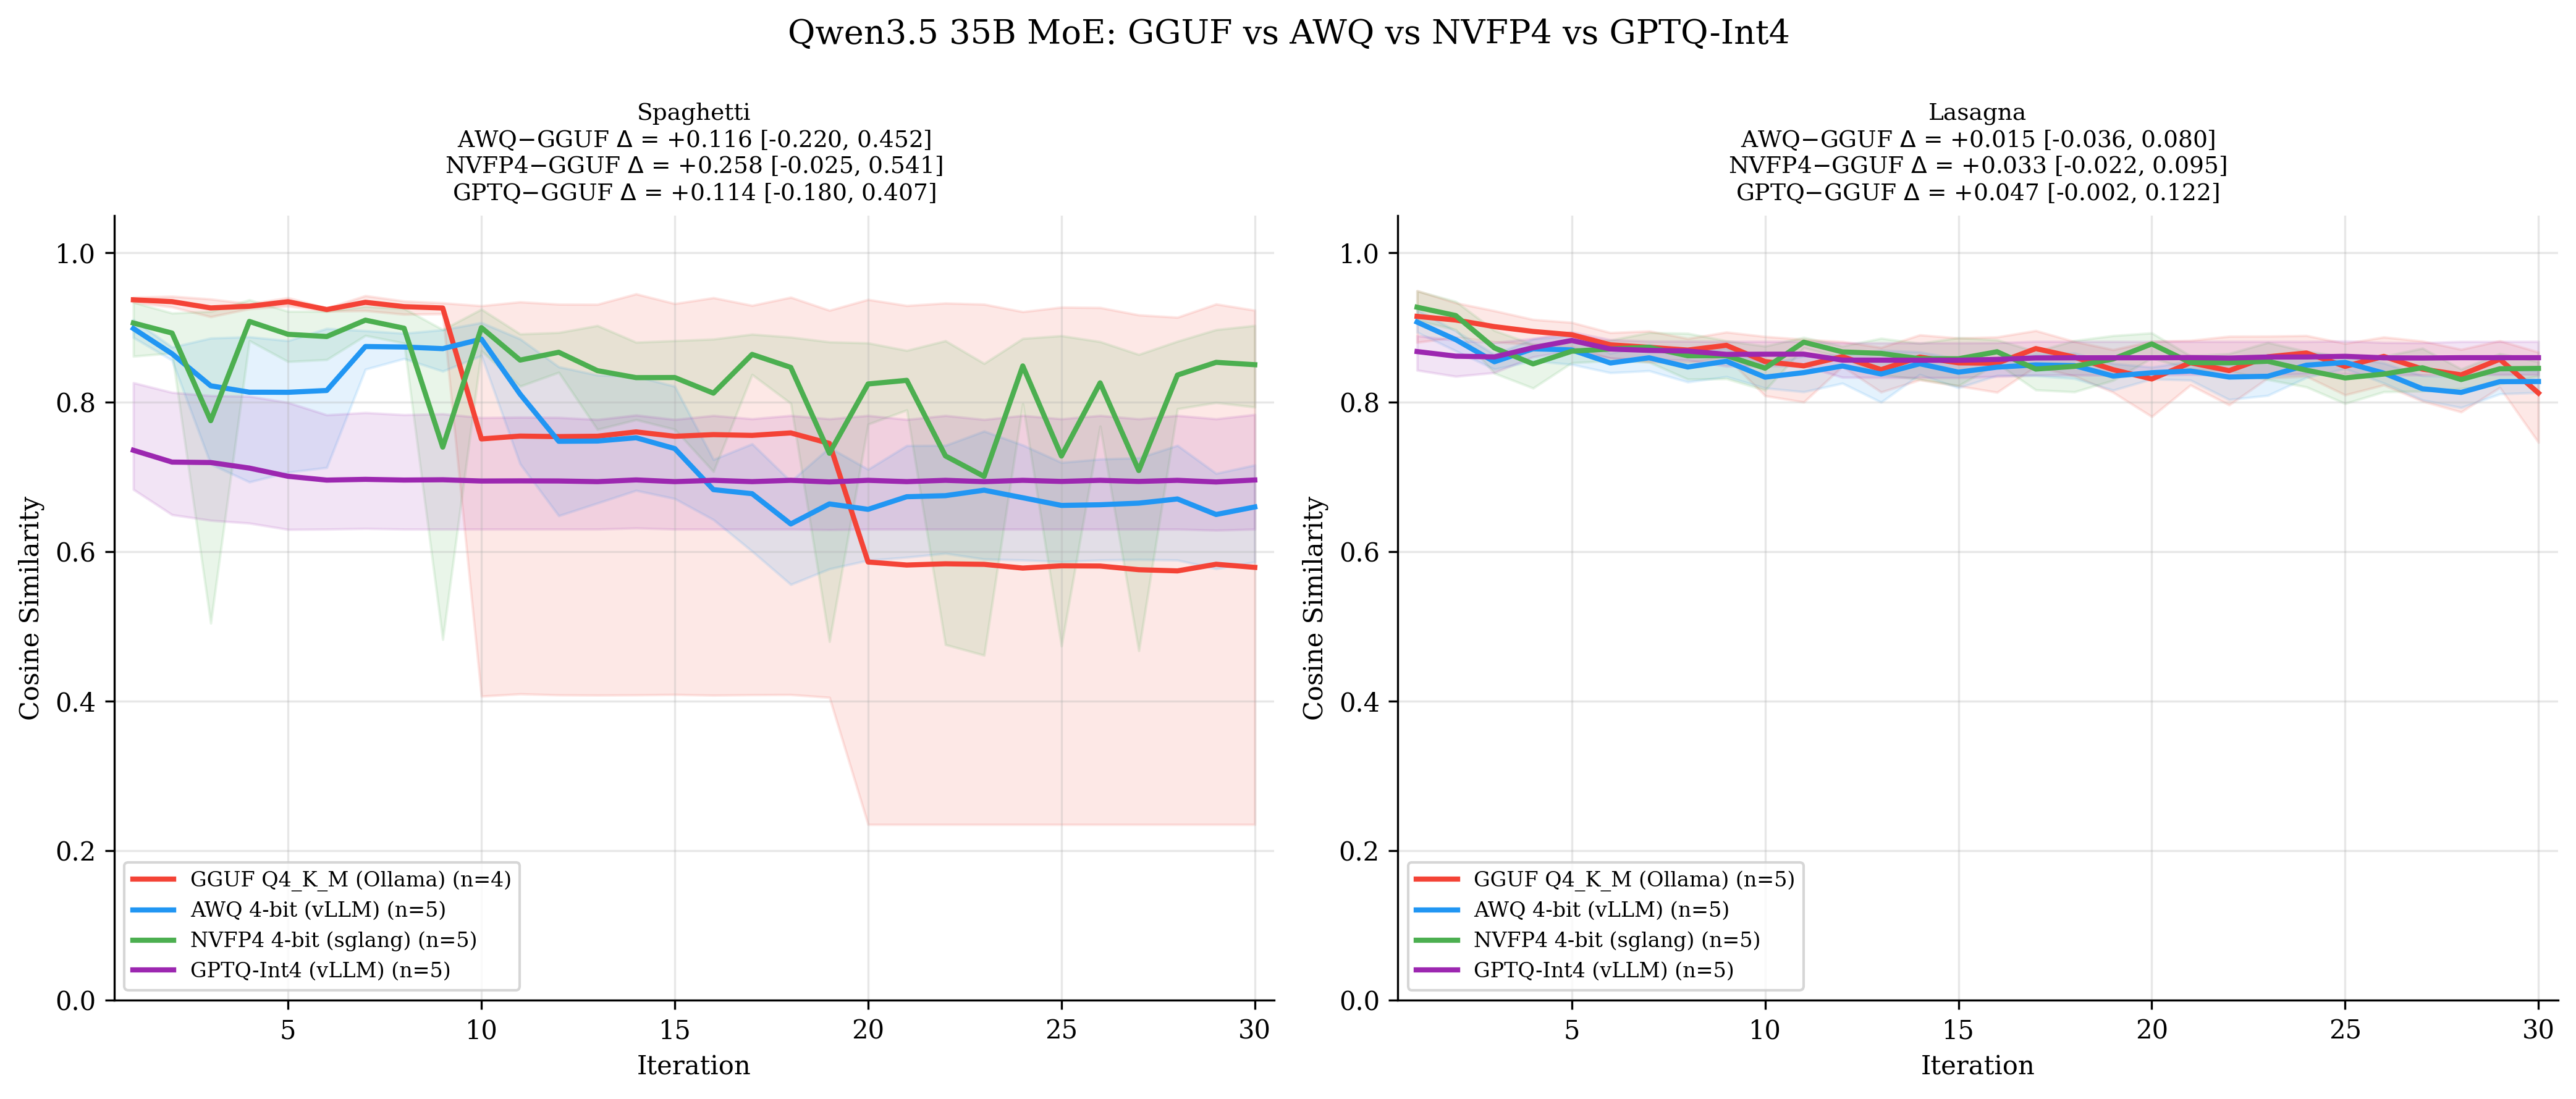
\includegraphics[width=\textwidth,height=0.31\textheight,keepaspectratio]{../results/qwen35_paper_figures/fig4_gguf_vs_awq.png}
\caption{Four quantization methods for the 35B MoE model: GGUF Q4\_K\_M
  (Ollama), AWQ 4-bit (vLLM), NVFP4 4-bit (SGLang), and GPTQ-Int4 (vLLM).
  Left: spaghetti. Right: lasagna. Panel titles give the seed-matched
  paired delta against GGUF with its bootstrap 95\% CI; $n$ per arm is
  shown in the legend.}
\label{fig:q35_formats}
\end{figure}

Table~\ref{tab:size_quant} and Figure~\ref{fig:q35_formats} give the result.
On the lasagna recipe the four formats are close: GGUF Q4\_K\_M 0.812, AWQ
0.828, NVFP4 0.845 and GPTQ-Int4 0.860, with seed-matched paired deltas
against GGUF of $+0.015$, $+0.033$ and $+0.047$ whose bootstrap intervals all
include zero, and no runaway chains in any arm. On the spaghetti recipe the
formats separate. Among clean chains GGUF Q4\_K\_M is best (0.923) and the
two vLLM formats are far below it (AWQ 0.660, CI [0.586, 0.716]; GPTQ-Int4
0.696, CI [0.630, 0.784]), a gap of 0.23--0.26 that is the largest
within-family effect in this paper apart from the capacity threshold. NVFP4
falls between (0.757), but on a single clean chain. The GGUF and NVFP4 clean
means rest on two and one chain respectively because those two arms lose
50\% and 80\% of their spaghetti chains to runaway thinking
(Section~\ref{sec:runaway}), while the vLLM arms lose none; the paired
deltas computed over all completed chains ($+0.116$ AWQ, $+0.258$ NVFP4,
$+0.114$ GPTQ, all intervals spanning zero at $n=4$ pairs) accordingly point
the other way. The format comparison on the short stimulus is thus a
trade: the GGUF build paraphrases most faithfully when it answers, and fails
to answer half the time.

Two further arms help separate format from serving stack. The 9B AWQ build
on vLLM behaves like the 35B AWQ build (spaghetti 0.683, lasagna 0.877 at
$T=0.7$) rather than like the 9B GGUF build (0.859, 0.830), so the
spaghetti penalty follows the format and stack, not the size. The
cross-family dataset shows the same divergence in a second family: the AWQ
and GGUF builds of Qwen3-VL~30B, both at 4-bit, produce different drift
dynamics (Section~\ref{sec:rq1}). Because the quantization algorithm and the
serving backend covary in three of the four arms, we attribute the effect to
the algorithm-and-stack combination rather than to either alone. The
practical conclusion does not depend on the attribution: 4-bit builds of the
same weights are not interchangeable in a drift-sensitive pipeline, and the
build that will be deployed is the one that must be benchmarked.


\subsection{KV Cache Precision}
\label{sec:rq2}

Figure~\ref{fig:rq2_deltas} shows the paired delta (fp16 $-$ q8\_0 KV cache)
for 10 Qwen3 models with bootstrap CIs and Wilcoxon $p$-values.

Key findings:
\begin{itemize}[leftmargin=*]
  \item The overall effect is not statistically significant
        (Wilcoxon $p = 0.375$, $n=10$), reflecting directionally mixed,
        model-dependent responses that cancel in aggregate.
  \item The per-model effects are directionally mixed rather than
        demonstrably non-monotonic: eight of the ten per-model delta
        confidence intervals include zero. Only 8B~q4\_K\_M
        ($+0.128$, CI $[0.050, 0.214]$) and 4B~Instruct~q4\_K\_M
        ($+0.011$, CI $[0.001, 0.022]$) have intervals excluding zero, and
        the latter is negligible in magnitude. With $n=5$ seed-matched
        pairs per model, the per-model $p$-values in Table~\ref{tab:rq2}
        should not be read as tests (Section~\ref{sec:stats}).
  \item Small models (0.6B) show the largest point improvement from fp16 KV
        ($+0.257$ and $+0.131$), consistent with KV cache noise
        disproportionately affecting models with fewer parameters, though
        both intervals span zero.
  \item The 80B model shows the largest point \emph{regression} with fp16
        KV ($-0.100$, CI $[-0.259, 0.079]$), which would be consistent with
        a latent attractor that q8 KV noise was masking; on this evidence
        the direction is suggestive rather than established.
  \item Among the q4\_K\_M models the deltas are small in magnitude,
        consistent with weight quantization noise dominating KV cache
        noise.
\end{itemize}

Figure~\ref{fig:rq2_heatmap} shows the heatmap of deltas across model
size and weight quantization. The magnitudes involved are an order below the
cross-family spread of Section~\ref{sec:rq1} and comparable to the temperature
effects of Section~\ref{sec:temperature}.

\begin{figure}[htbp]
  \centering
  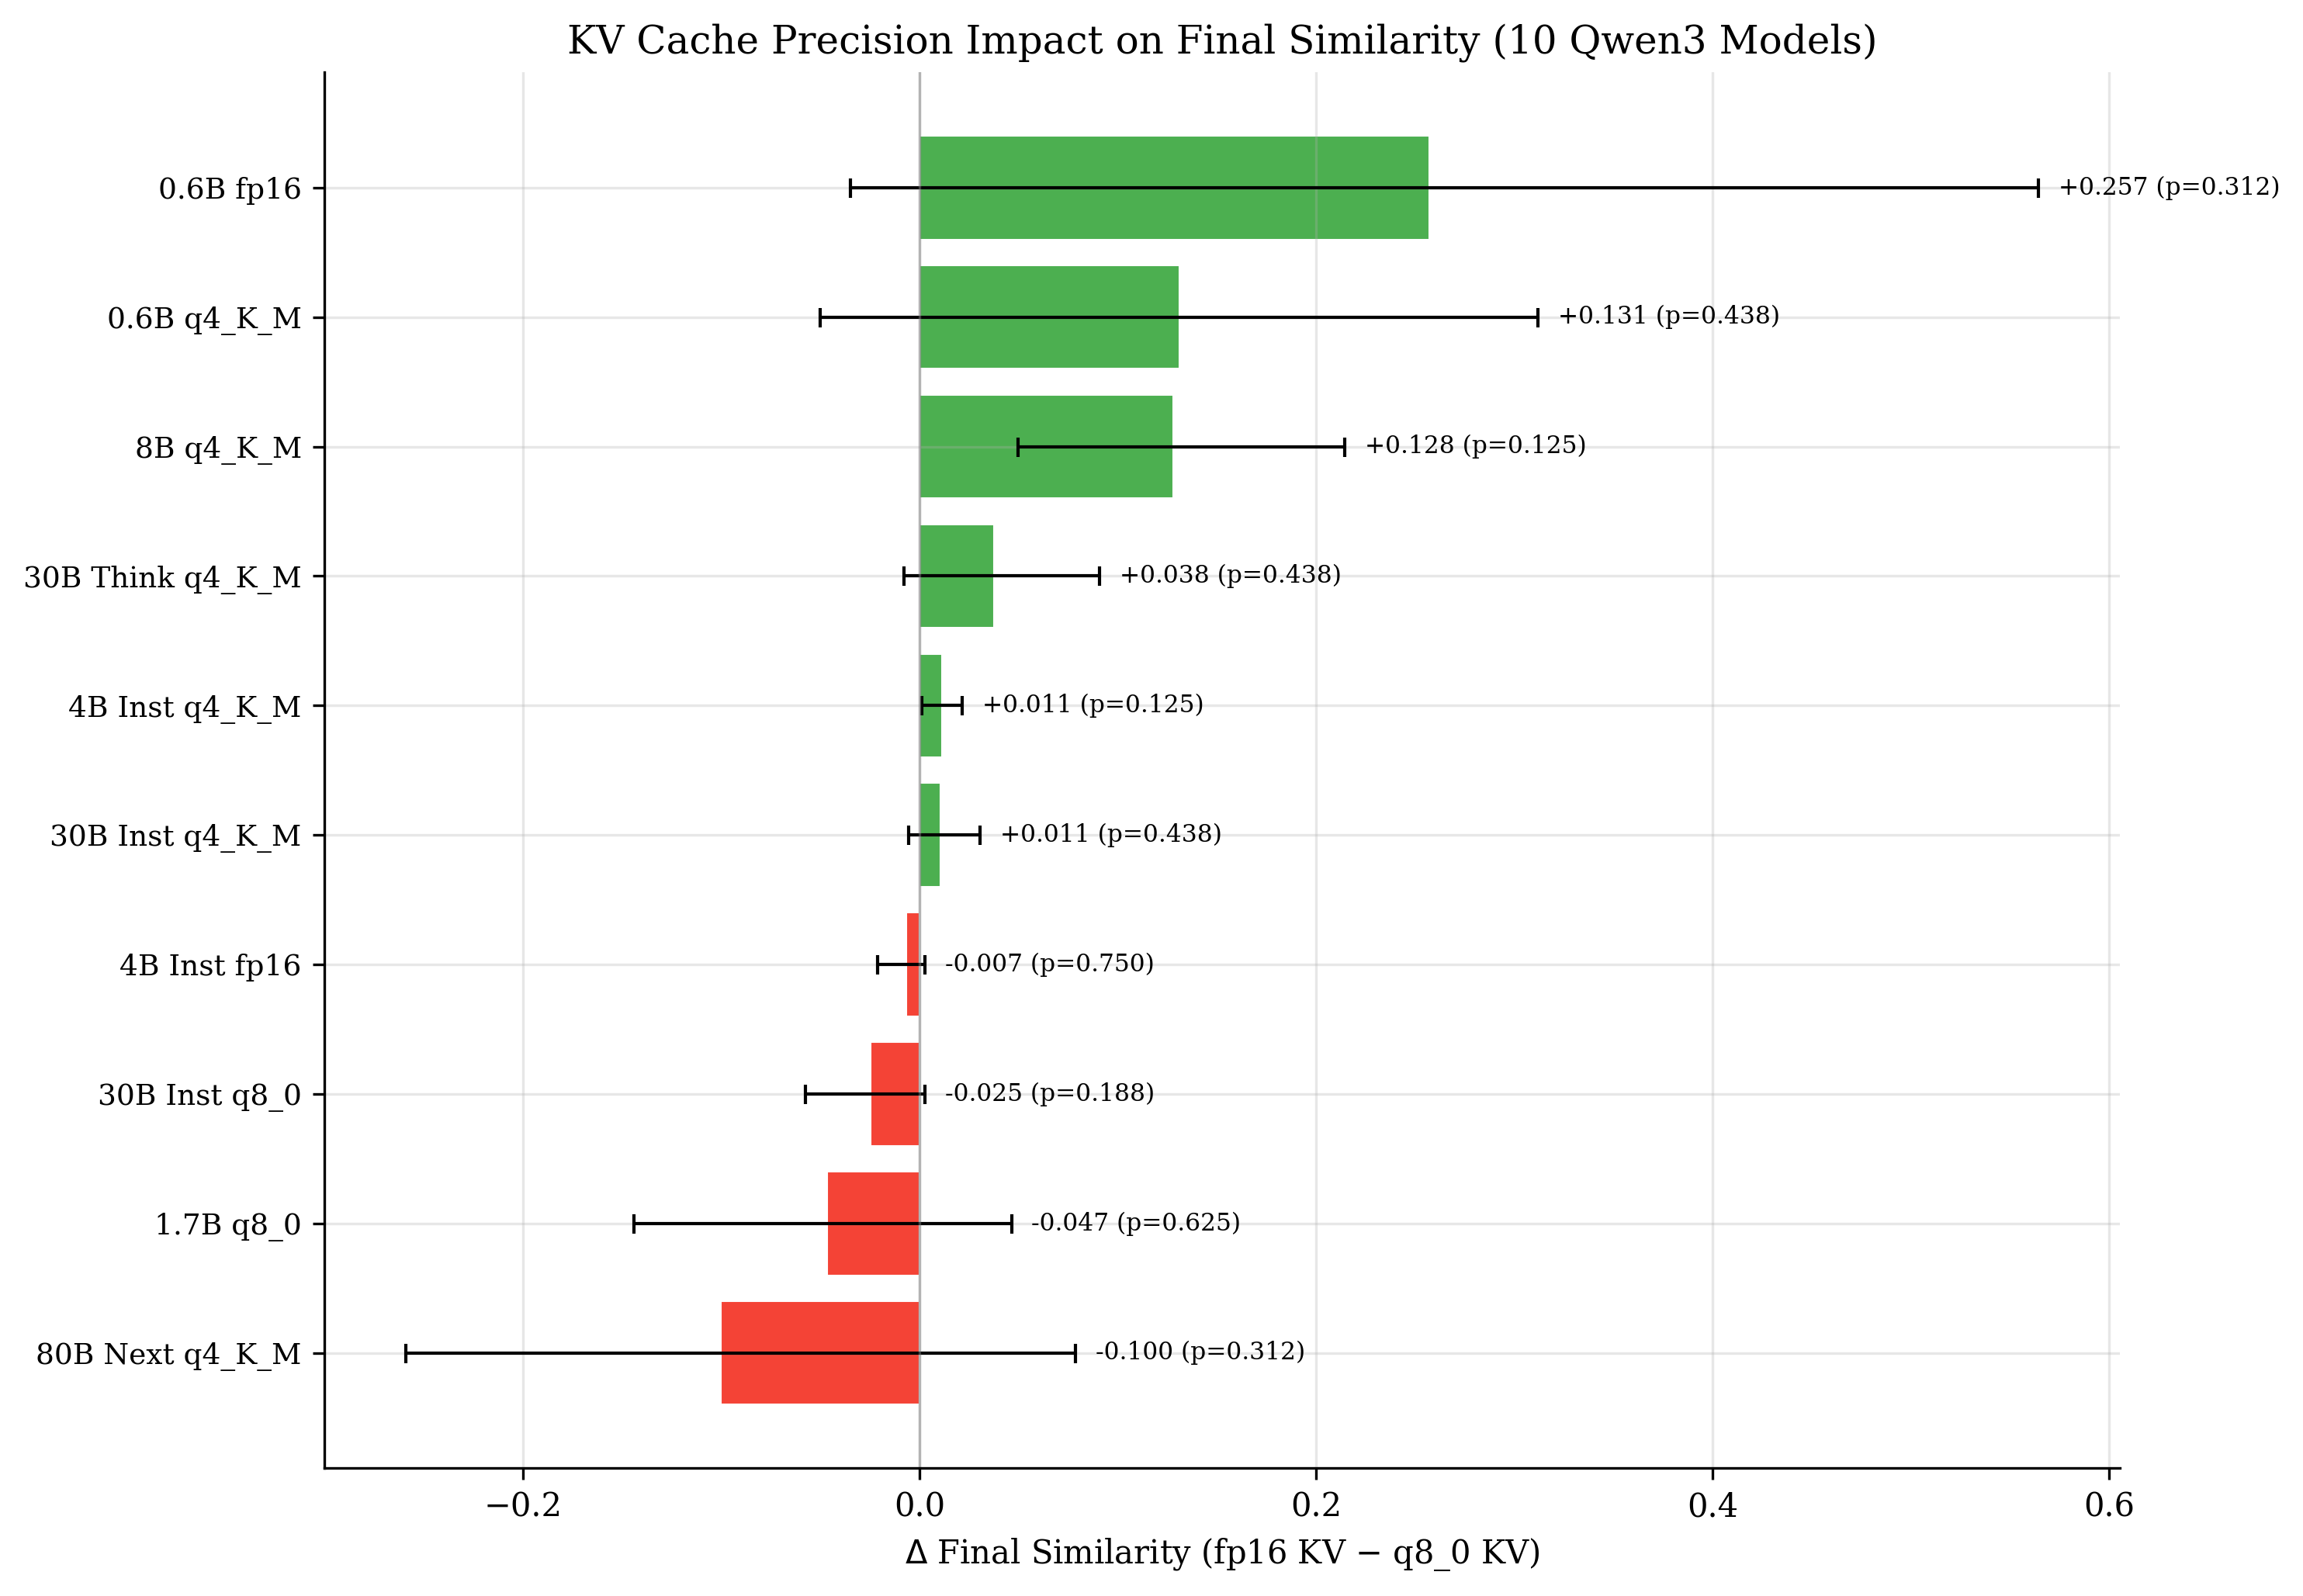
\includegraphics[width=\textwidth,height=0.31\textheight,keepaspectratio]{../results/paper_figures/fig3_rq2_delta_bars.png}
  \caption{KV cache precision impact (fp16 $-$ q8\_0) on final similarity.
  Error bars show 95\% bootstrap CI. Green = improvement, red = regression.
  Annotated with Wilcoxon $p$-values.}
  \label{fig:rq2_deltas}
\end{figure}

\begin{figure}[htbp]
  \centering
  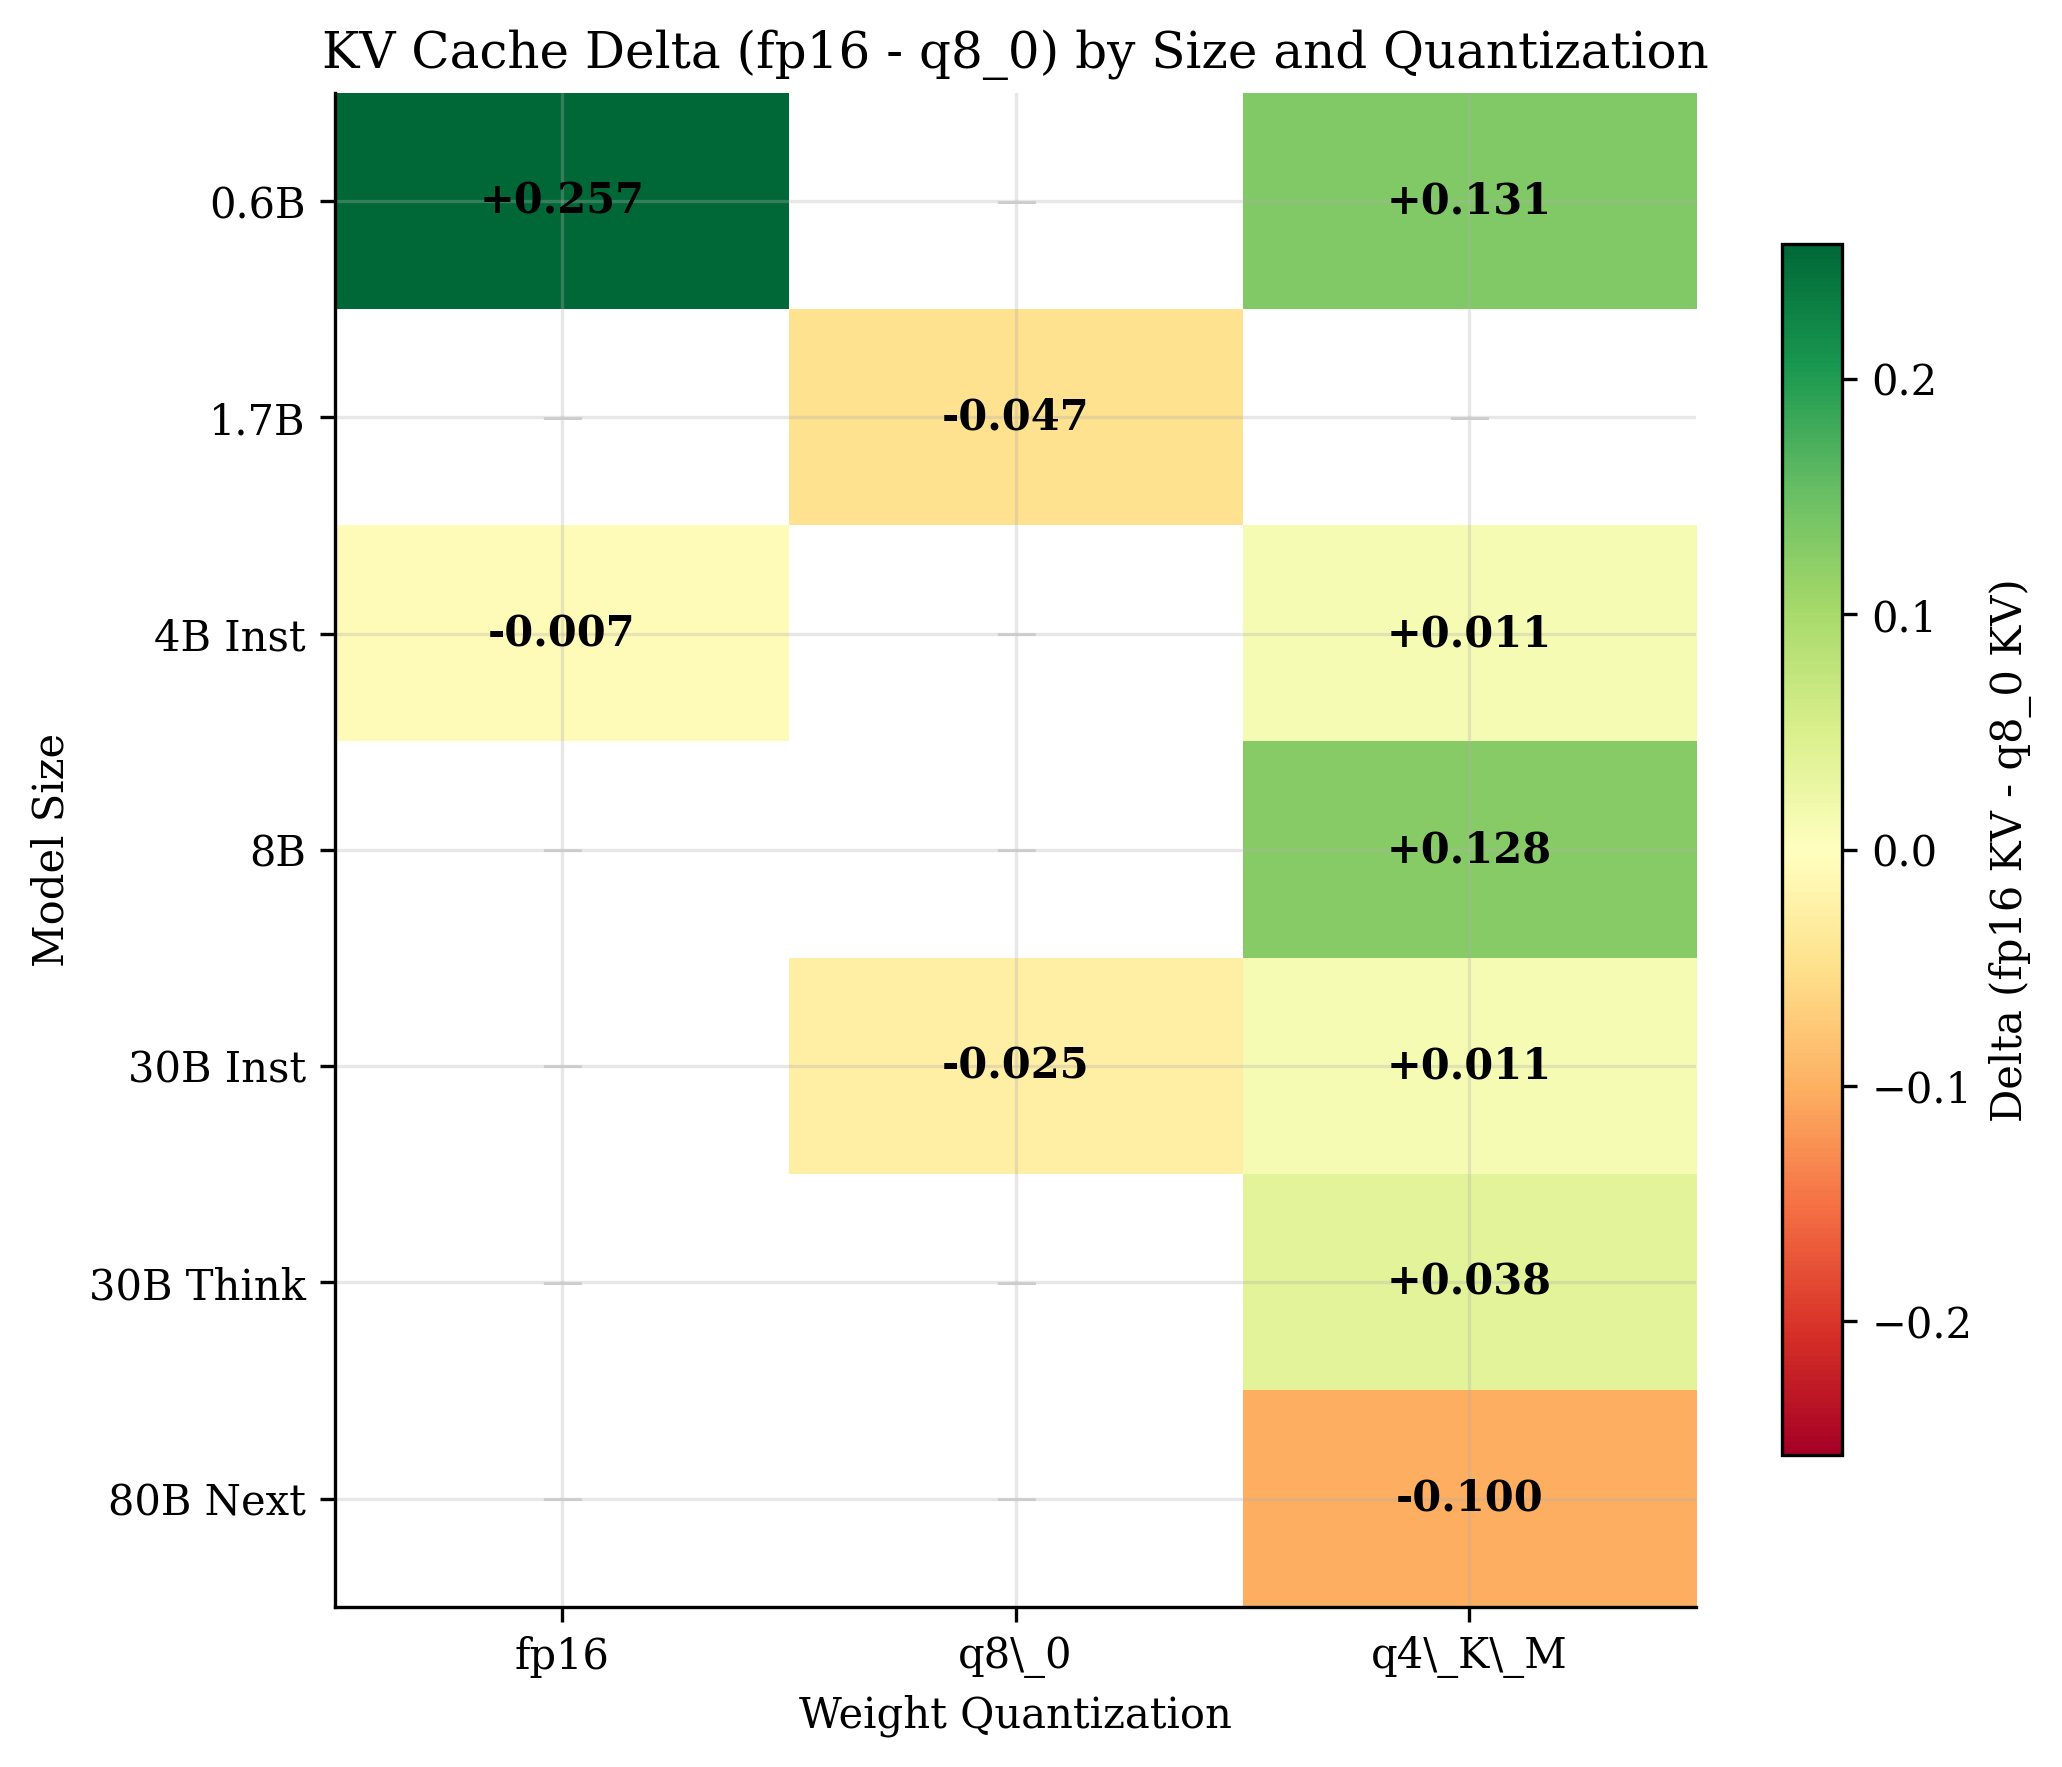
\includegraphics[width=\textwidth,height=0.31\textheight,keepaspectratio]{../results/paper_figures/fig4_rq2_heatmap.png}
  \caption{KV cache precision delta across model size and weight quantization.
  Green = fp16 KV helped; red = hurt. Blank cells indicate untested combinations.}
  \label{fig:rq2_heatmap}
\end{figure}

\begin{table}[t]
\centering
\caption{KV cache precision effects (RQ2). Paired delta = fp16 KV $-$ q8\_0 KV
  on final cosine similarity, 5 seed-matched pairs per model, with the
  bootstrap 95\% CI of the delta ($B=10{,}000$). With $n=5$ pairs the
  two-sided Wilcoxon signed-rank test cannot return a $p$ below 0.125,
  so the $p$ column is reported for completeness only and no per-model
  test here is capable of reaching $p<0.05$; the delta CIs are the
  informative quantity.}
\label{tab:rq2}
\small
\begin{tabular}{llccccll}
\toprule
Model & Size & Quant & q8 Mean & fp16 Mean & $\Delta$ & 95\% CI of $\Delta$ & $p$ \\
\midrule
0.6B fp16 & 0.6B & fp16 & 0.577 & 0.834 & +0.257 & [-0.035, 0.564] & 0.312 \\
0.6B q4\_K\_M & 0.6B & q4\_K\_M & 0.674 & 0.805 & +0.131 & [-0.050, 0.312] & 0.438 \\
8B q4\_K\_M & 8B & q4\_K\_M & 0.731 & 0.858 & +0.128 & [0.050, 0.214] & 0.125 \\
30B Think q4\_K\_M & 30B Think & q4\_K\_M & 0.742 & 0.779 & +0.038 & [-0.008, 0.091] & 0.438 \\
4B Inst q4\_K\_M & 4B Inst & q4\_K\_M & 0.918 & 0.929 & +0.011 & [0.001, 0.022] & 0.125 \\
30B Inst q4\_K\_M & 30B Inst & q4\_K\_M & 0.907 & 0.917 & +0.011 & [-0.005, 0.031] & 0.438 \\
4B Inst fp16 & 4B Inst & fp16 & 0.897 & 0.890 & -0.007 & [-0.021, 0.003] & 0.750 \\
30B Inst q8\_0 & 30B Inst & q8\_0 & 0.912 & 0.887 & -0.025 & [-0.057, 0.003] & 0.188 \\
1.7B q8\_0 & 1.7B & q8\_0 & 0.767 & 0.720 & -0.047 & [-0.144, 0.046] & 0.625 \\
80B Next q4\_K\_M & 80B Next & q4\_K\_M & 0.609 & 0.508 & -0.100 & [-0.259, 0.079] & 0.312 \\
\bottomrule
\end{tabular}
\end{table}



\subsection{Temperature}
\label{sec:temperature}

Temperature was ablated in both datasets. Figure~\ref{fig:temperature} shows
the cross-family interaction between temperature and model, and
Figure~\ref{fig:q35_temp} the within-family version across eight Qwen3.5
configurations (4 Ollama GGUF, the 35B AWQ, NVFP4 and GPTQ-Int4 variants, the
9B AWQ variant, and the Nemotron control).

\paragraph{Cross-family observations.}
\begin{itemize}[leftmargin=*]
  \item $T=0$ (greedy decoding) does not guarantee stability: catastrophic models
        still drift, confirming that drift is not merely a function of sampling noise.
  \item Stable models (qwen3:30b-instruct) are robust across all temperatures.
  \item Unstable models (llama3.1:8b) are sensitive to temperature, with higher
        temperatures accelerating collapse.
  \item The relationship is non-linear: moderate temperatures ($T=0.3$--$0.5$)
        sometimes \emph{improve} stability relative to $T=0$, suggesting that
        some sampling diversity can help escape local attractors.
\end{itemize}

\begin{figure}[htbp]
  \centering
  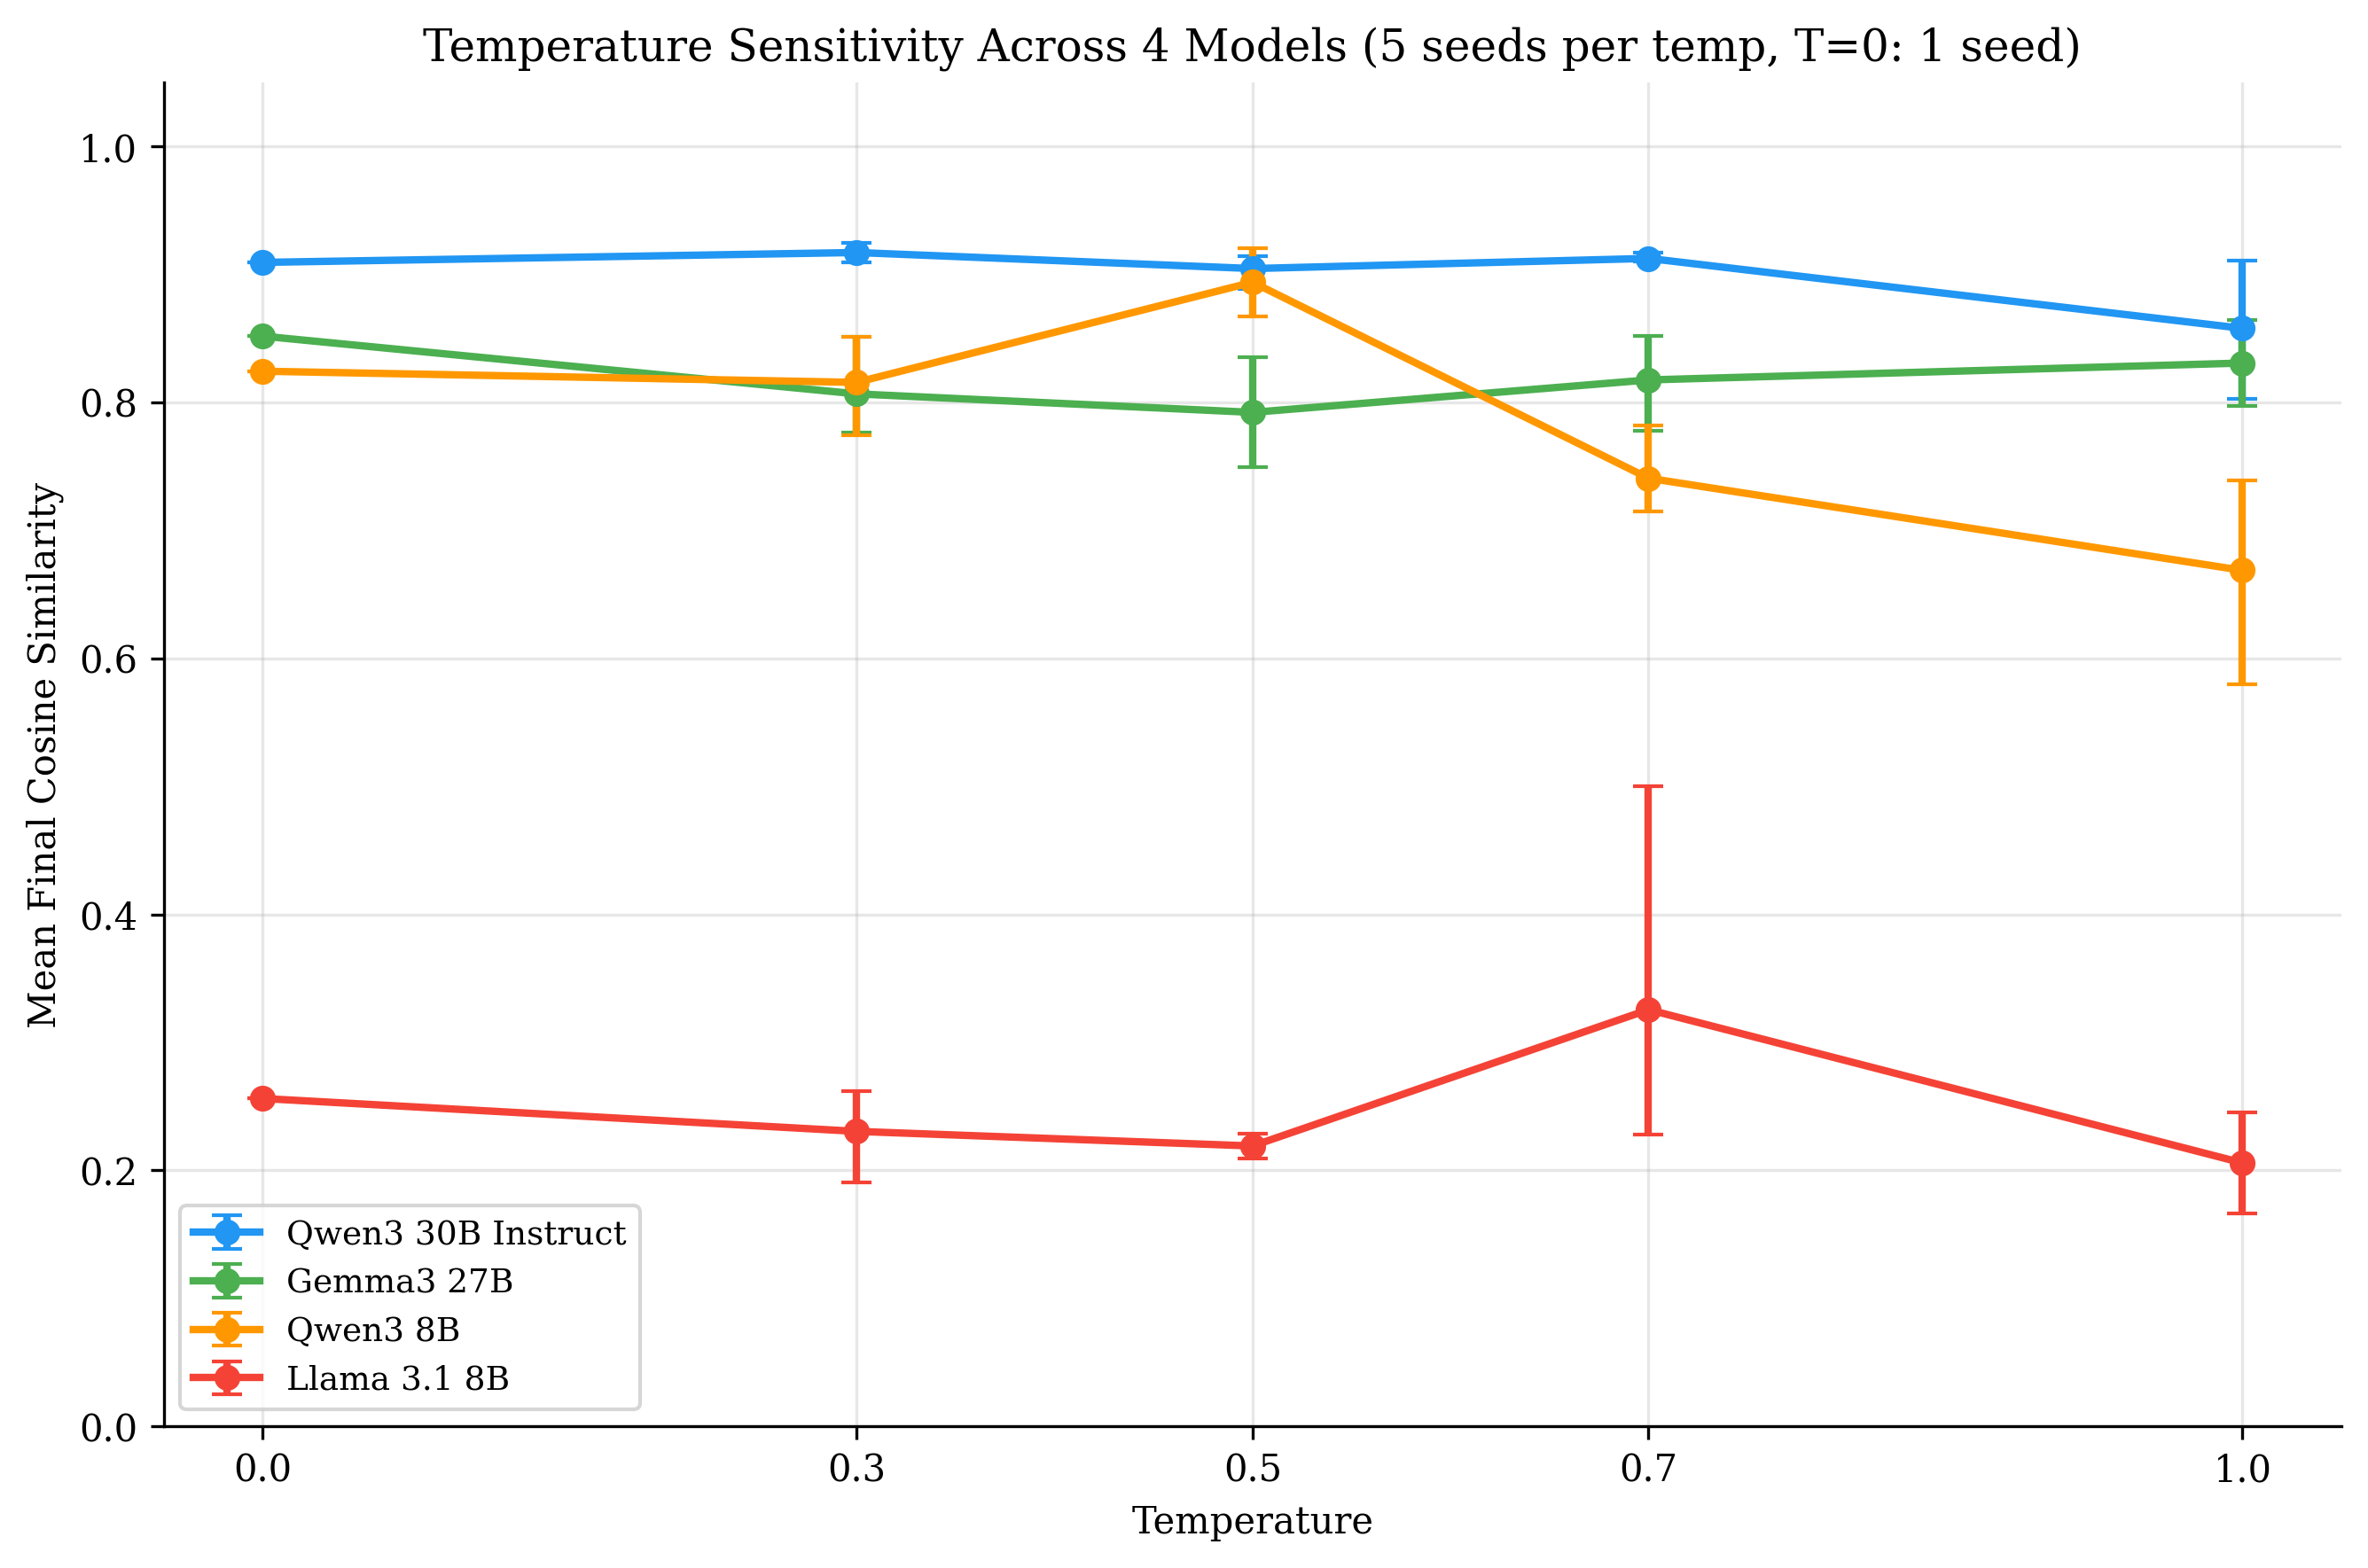
\includegraphics[width=\textwidth,height=0.31\textheight,keepaspectratio]{../results/paper_figures/fig9_temperature.png}
  \caption{Temperature sensitivity across 4 cross-family models. Error bars show
  95\% CI (5 seeds; $T=0$ is deterministic, single run). Drift is not reducible
  to sampling entropy.}
  \label{fig:temperature}
\end{figure}

\begin{figure}[htbp]
\centering
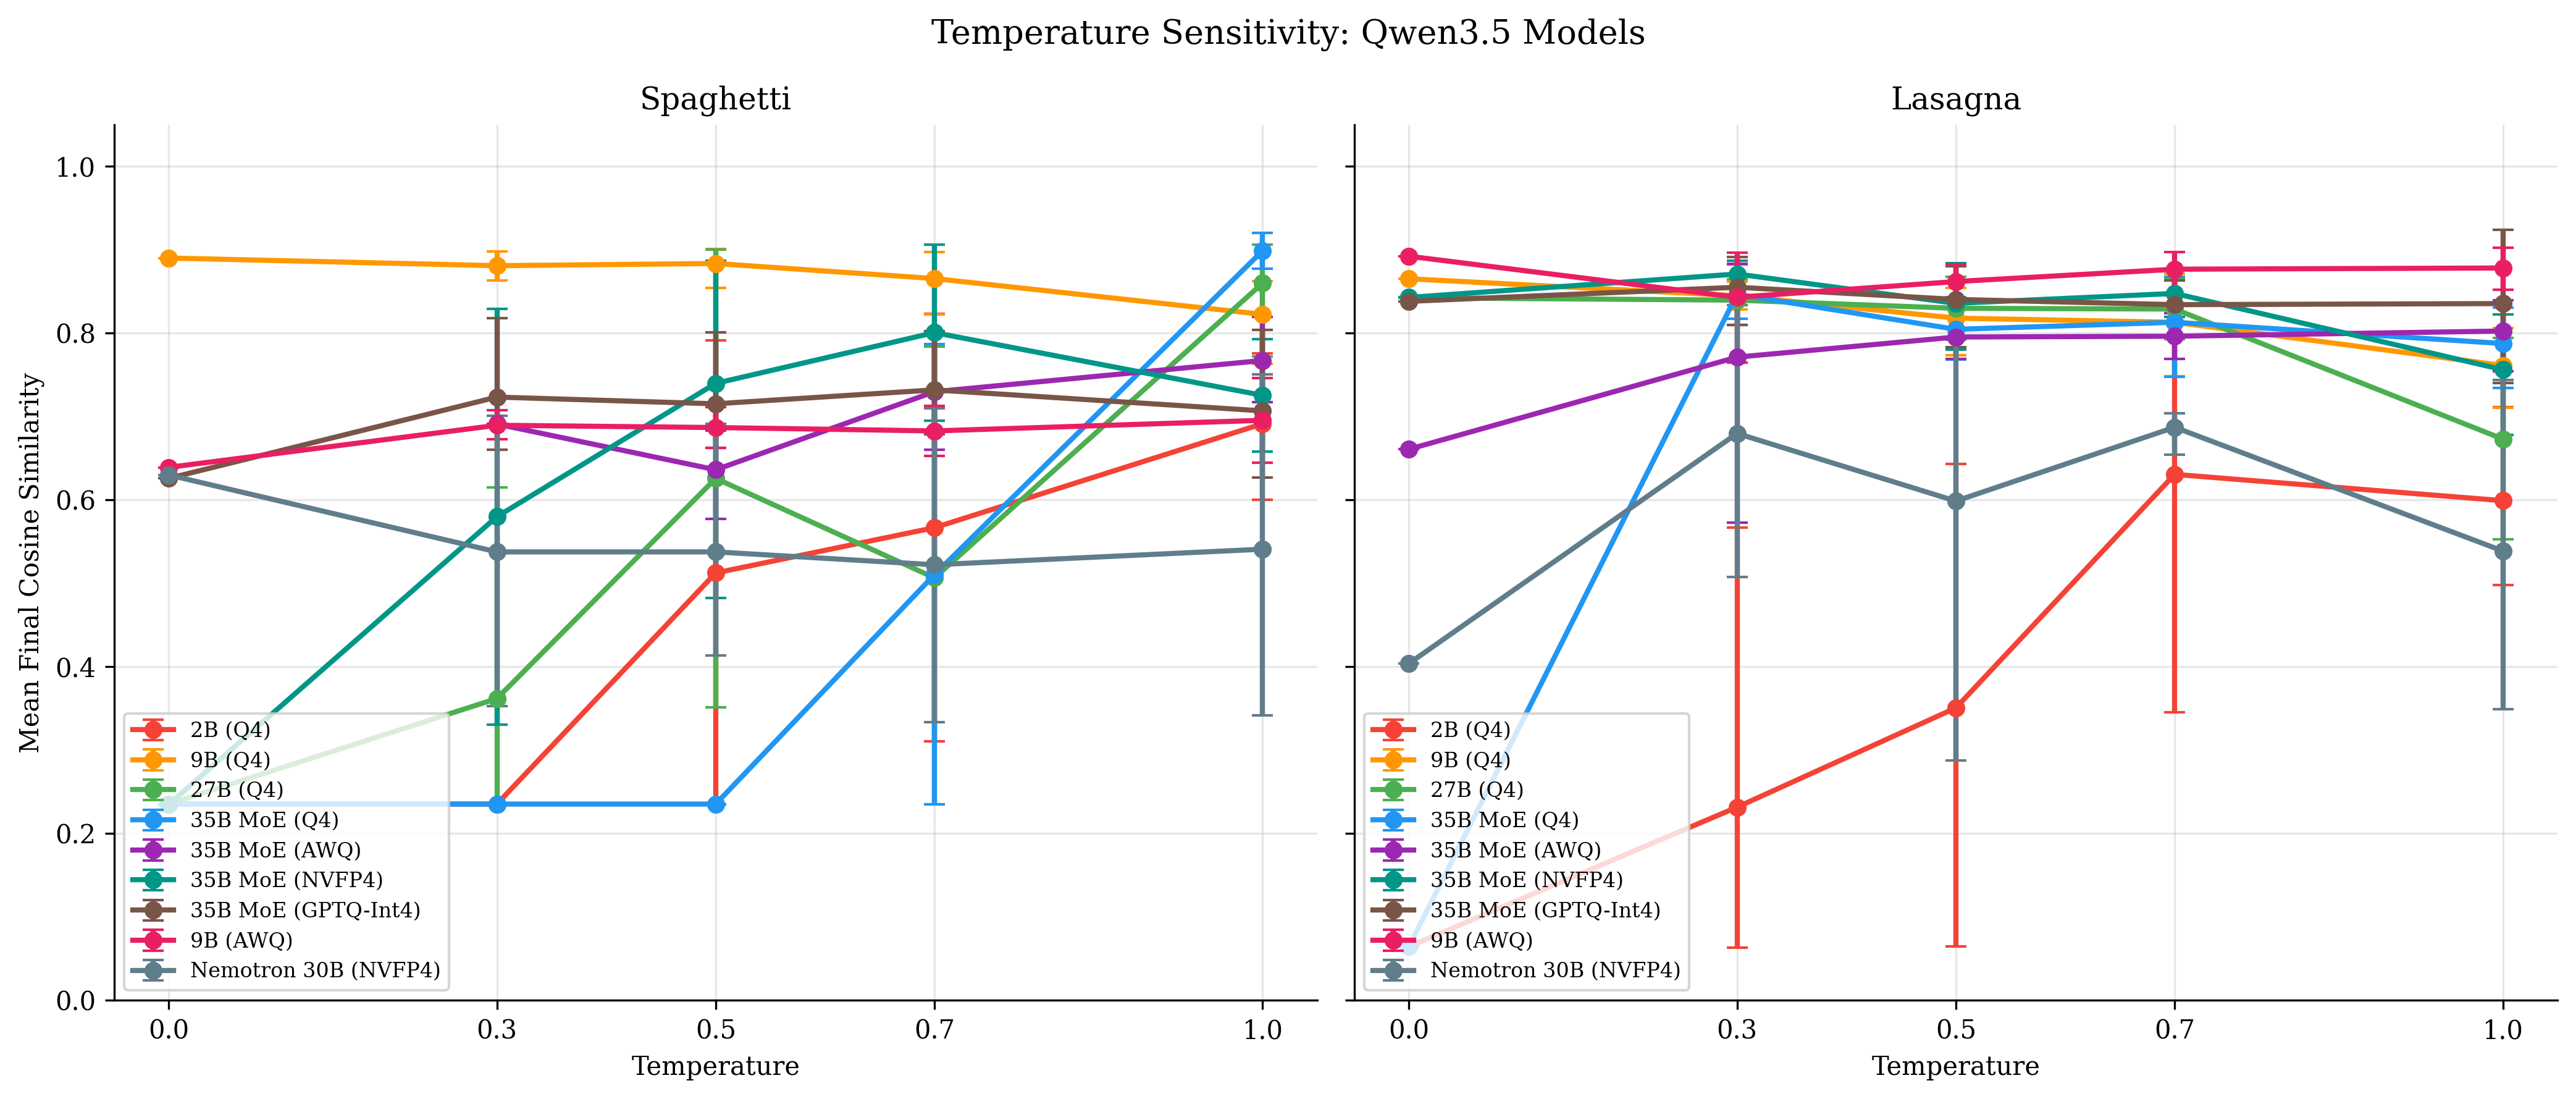
\includegraphics[width=\textwidth,height=0.31\textheight,keepaspectratio]{../results/qwen35_paper_figures/fig5_temperature.png}
\caption{Temperature sensitivity across Qwen3.5 configurations. Left: spaghetti.
  Right: lasagna.}
\label{fig:q35_temp}
\end{figure}

\paragraph{Size-dependent sensitivity within the family.}
The 9B GGUF model shows remarkable temperature insensitivity: final
similarity ranges only 0.823--0.890 across $T \in [0.0, 1.0]$ on
spaghetti. In contrast, the 2B model shows \emph{inverted} temperature
sensitivity on spaghetti: $T=0.0$ and $T=0.3$ both sit at the
empty-output floor of 0.235, and similarity then rises monotonically with
temperature (0.512 at $T=0.5$, 0.567 at $T=0.7$, 0.691 at $T=1.0$). The
same inversion appears for the 35B MoE GGUF model, which is pinned at
0.235 for $T \leq 0.5$ and reaches 0.899 at $T=1.0$. This
suggests that low-temperature deterministic sampling can trap small models
in repetitive attractor loops that the embedding model scores favorably,
while moderate temperatures disrupt this lock-in without providing enough
diversity to maintain content.

\paragraph{Format-dependent temperature profiles.}
The 35B AWQ model shows a qualitatively different pattern: similarity
\emph{increases} with temperature on both recipes (spaghetti: 0.636 at
$T=0.5$ to 0.767 at $T=1.0$; lasagna: 0.661 at $T=0.0$ to 0.803 at
$T=1.0$; the AWQ $T=0.0$ spaghetti chain was among those lost to the
failed rerun). The 35B GPTQ-Int4 and 9B AWQ variants are by contrast
nearly flat across the whole temperature range (GPTQ spaghetti
0.626--0.732; 9B~AWQ spaghetti 0.639--0.696). This is the
opposite of the conventional expectation that higher temperature increases
randomness and thus drift. We hypothesize that AWQ quantization
creates a restricted output distribution at low temperatures, and higher
temperature helps the model access more of its learned paraphrase space.


\clearpage
\subsection{System Prompts: Complexity Threshold and Rank Inversion}
\label{sec:rq3}

The same 20 system prompts (Appendix~\ref{app:prompts}) were run in both
datasets: across families on 30B AWQ and 8B q4\_K\_M, and within the Qwen3.5
family on six configurations---9B and 27B GGUF, 35B AWQ, 35B NVFP4, 35B
GPTQ-Int4 and 9B AWQ---plus the out-of-family Nemotron-3-Nano-30B control.
Each condition uses up to 5 completed chains on both recipes.
Table~\ref{tab:rq4_spread} summarizes the per-configuration spread, best and
worst prompt, and the pairwise Spearman rank correlations, and
Table~\ref{tab:sysprompt} gives the per-prompt means.

\paragraph{Complexity threshold.}
Figure~\ref{fig:complexity} shows that on the 3-step spaghetti recipe, all 20
system prompts produce nearly identical drift (spread $< 0.01$ on 30B AWQ).
On the 21-step lasagna recipe, the spread increases to $\sim$0.054, revealing
a \emph{complexity threshold} below which prompt engineering is invisible.

\paragraph{Prompt effectiveness.}
Figure~\ref{fig:hero_lasagna} shows drift trajectories for all 20 system prompts
on the 30B AWQ model with lasagna, and Figure~\ref{fig:q35_syshero} the
corresponding within-family view on Qwen3.5 27B GGUF. The best-performing
prompts on 30B AWQ (Multi-Agent Relay, No Meta Ever) target a specific failure
mode: meta-commentary about the relay task itself. Over-constraining
(Ultra-Constrained Fidelity) backfires, producing the worst performance.

\paragraph{Cross-model rank inversion.}
Figure~\ref{fig:cross_model} reveals that prompt rankings on 30B AWQ are
essentially uncorrelated with rankings on 8B q4\_K\_M
(Spearman $\rho = 0.15$, $p = 0.53$, 95\% CI $[-0.37, 0.61]$), so prompt
optimization does not transfer across families.
Figure~\ref{fig:q35_syscross} extends the same analysis within one family and
across quantization formats of one checkpoint.

\begin{figure}[htbp]
  \centering
  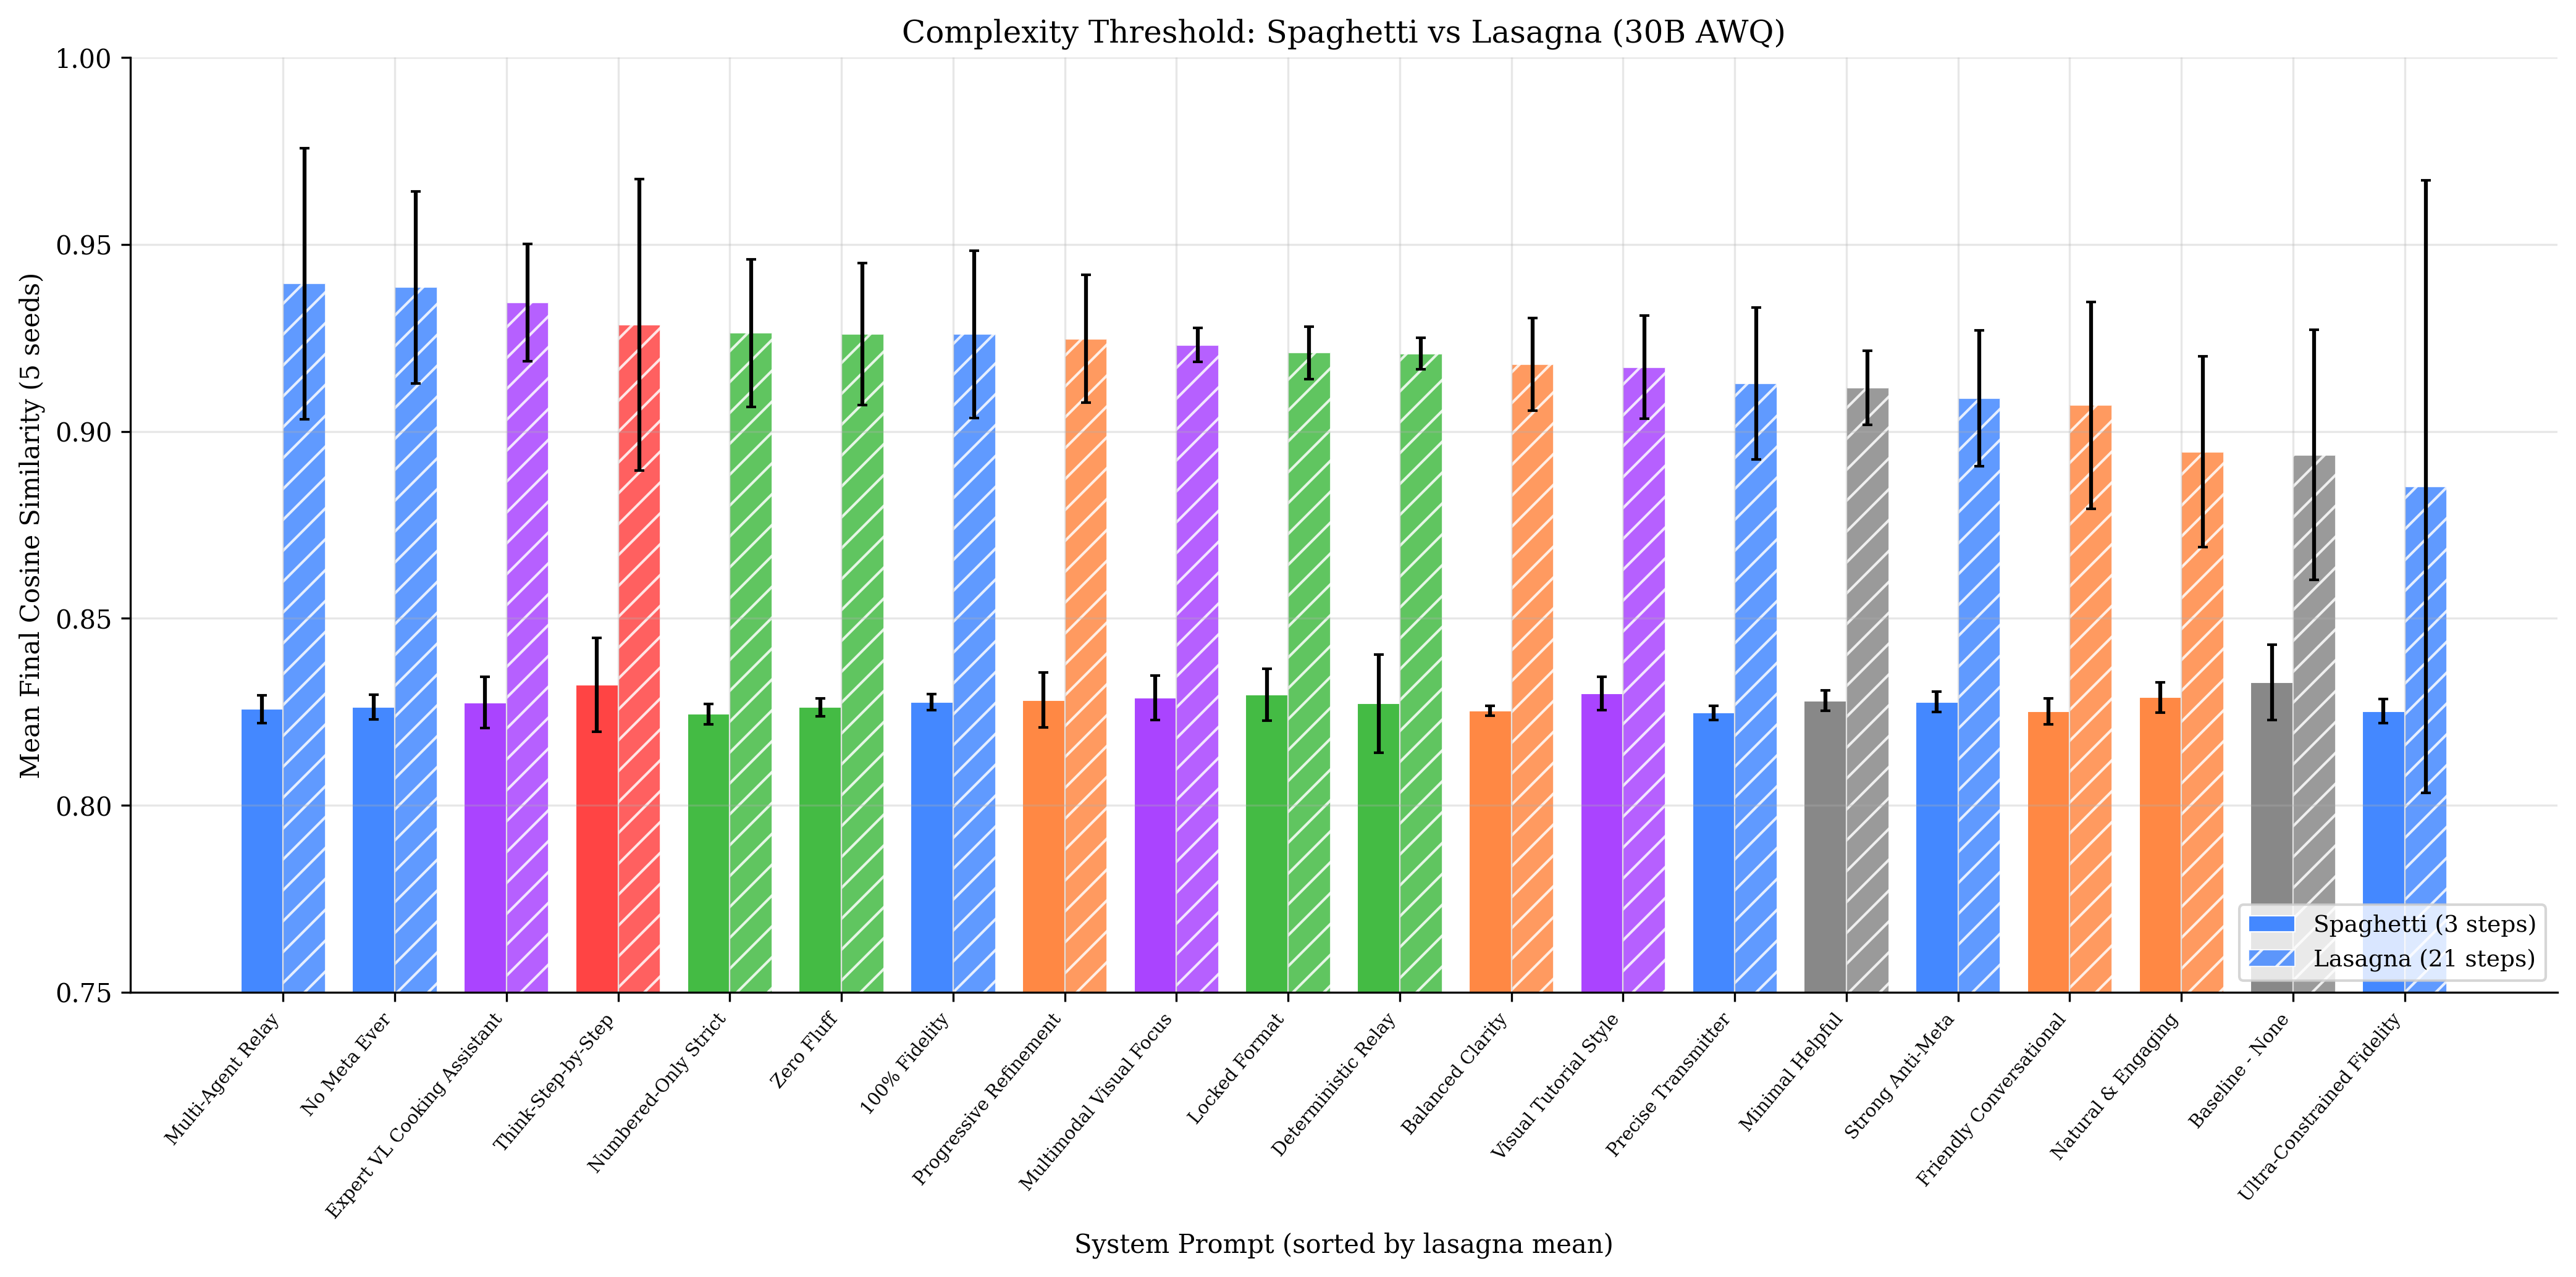
\includegraphics[width=\textwidth,height=0.31\textheight,keepaspectratio]{../results/paper_figures/fig5_complexity_threshold.png}
  \caption{Complexity threshold: system prompts are invisible on the 3-step recipe
  (solid bars) but differentiate on the 21-step recipe (hatched bars). 30B AWQ, 5 seeds.}
  \label{fig:complexity}
\end{figure}

\begin{figure}[htbp]
  \centering
  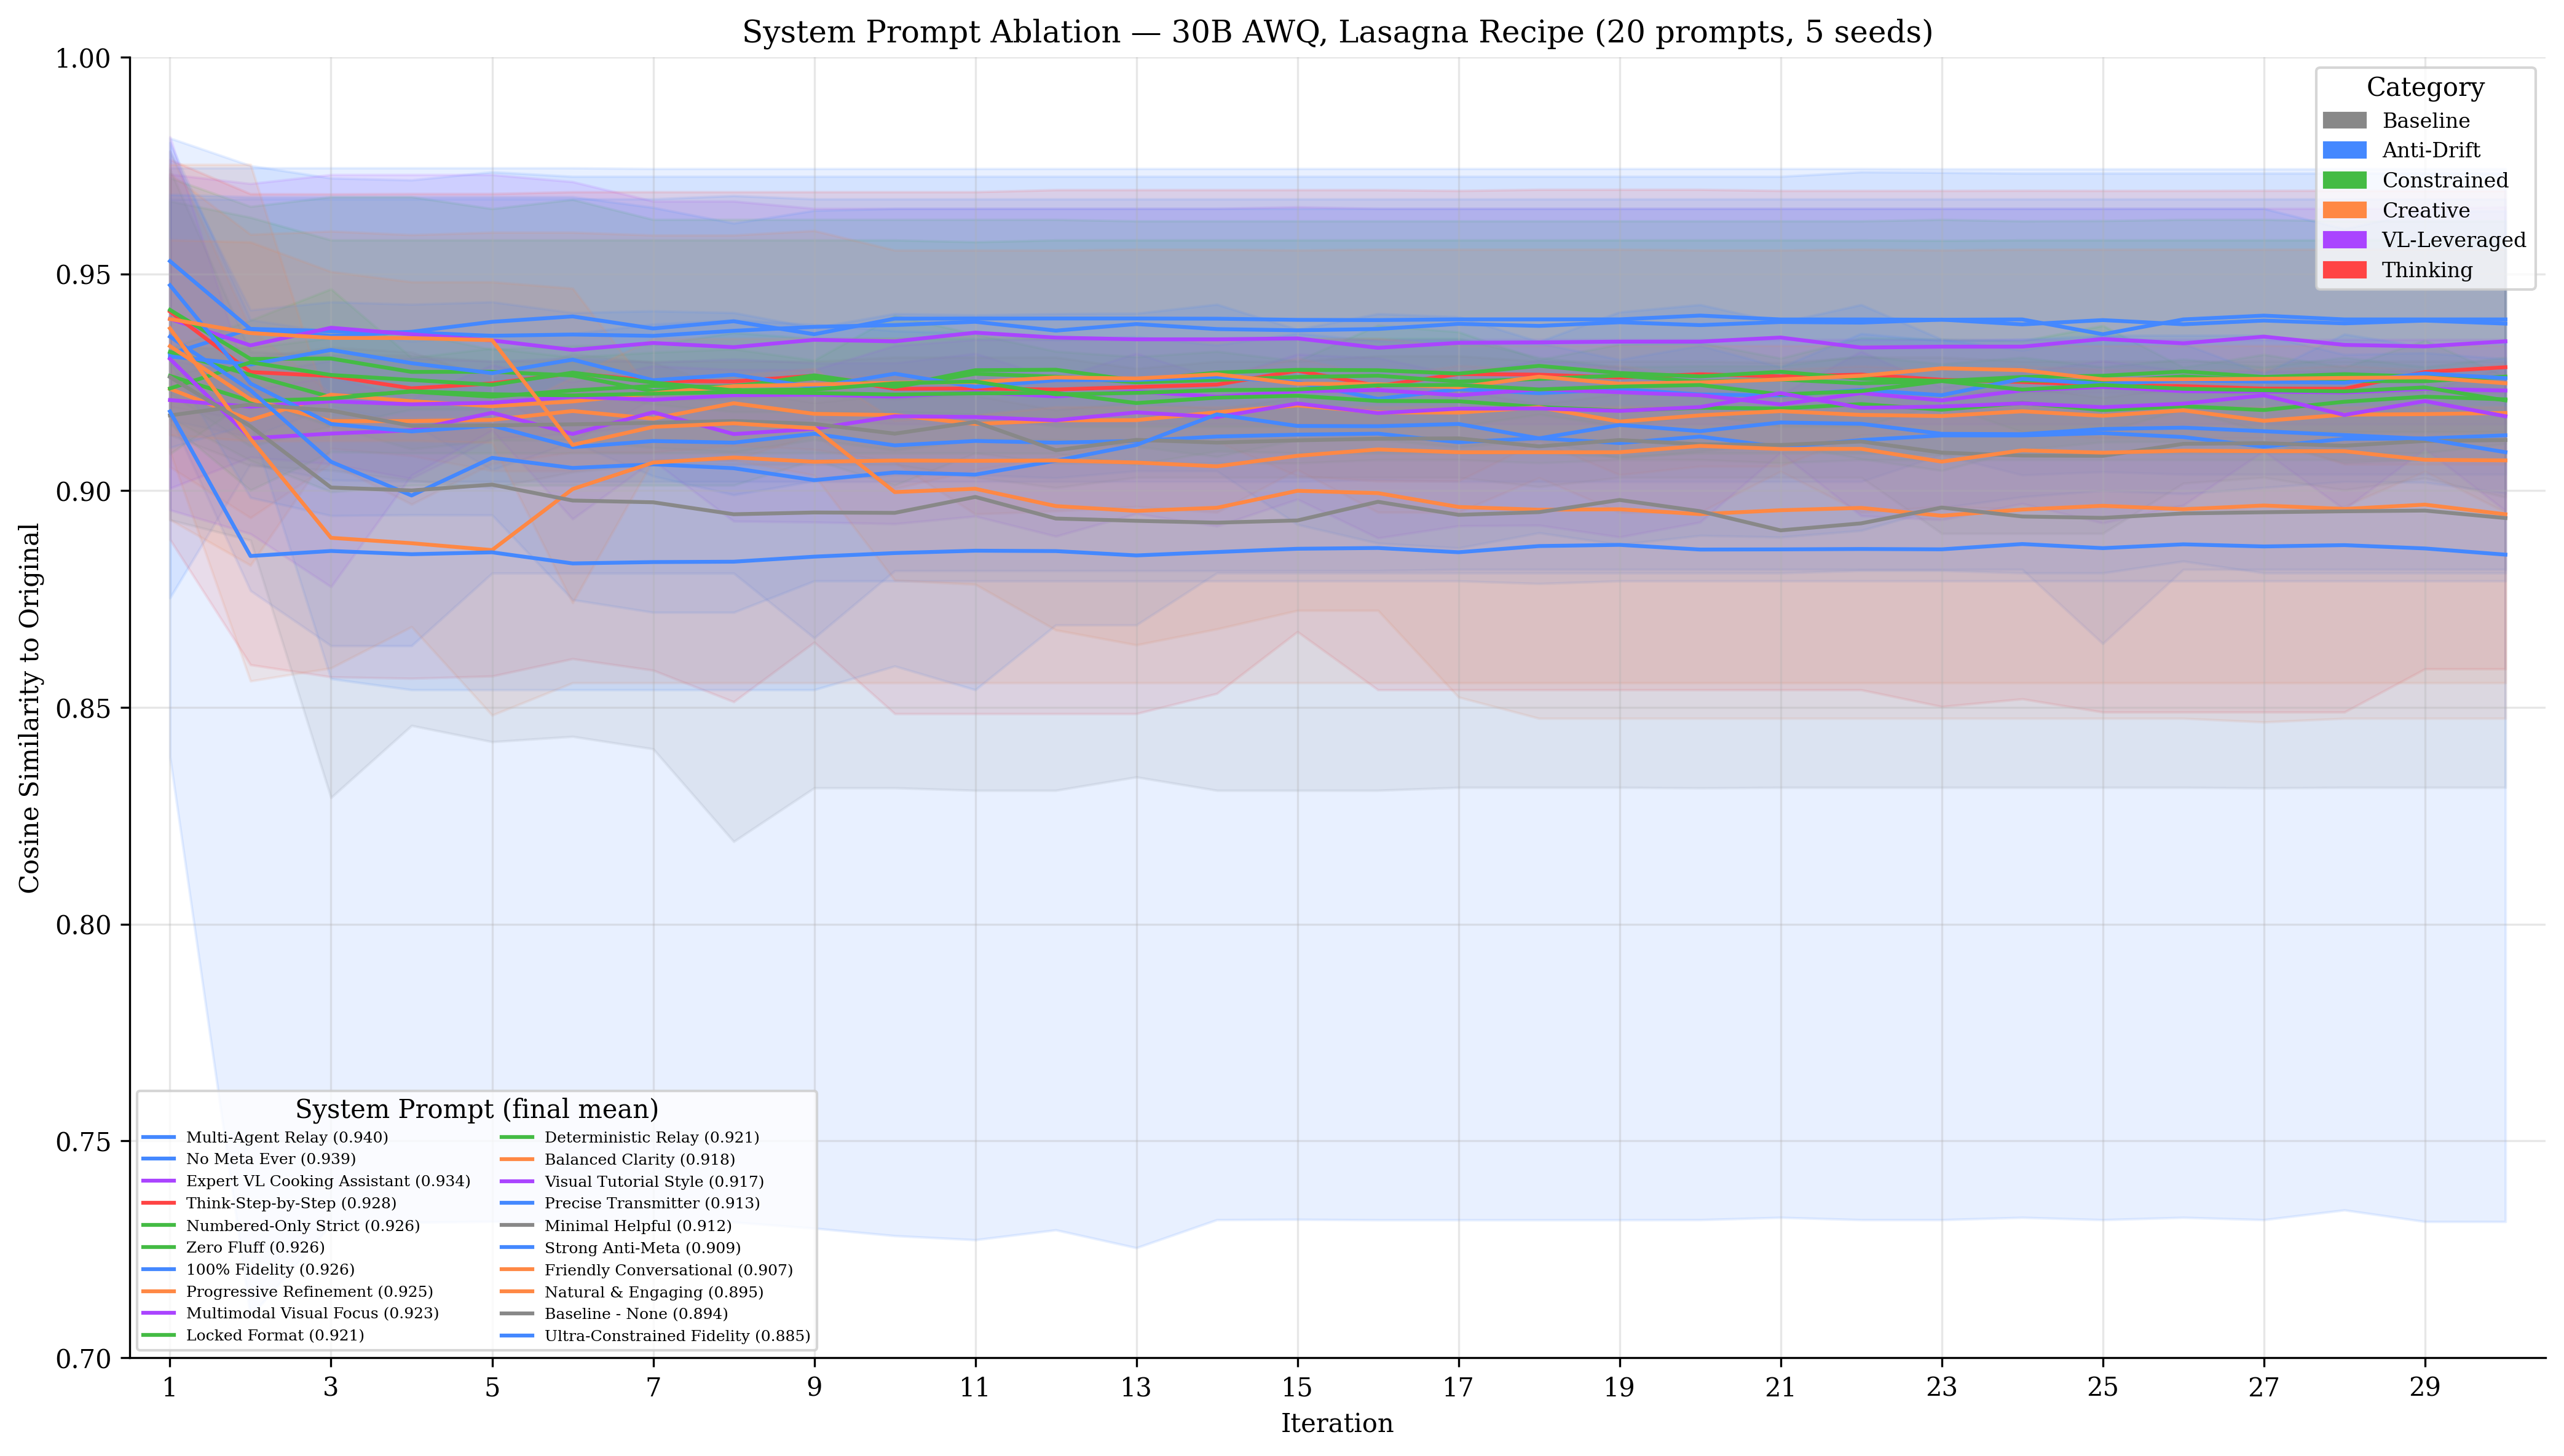
\includegraphics[width=\textwidth,height=0.31\textheight,keepaspectratio]{../results/paper_figures/fig6_hero_lasagna.png}
  \caption{System prompt ablation on 30B AWQ, lasagna recipe. Lines colored by
  category; shaded = min/max across 5 seeds.}
  \label{fig:hero_lasagna}
\end{figure}

\begin{figure}[htbp]
\centering
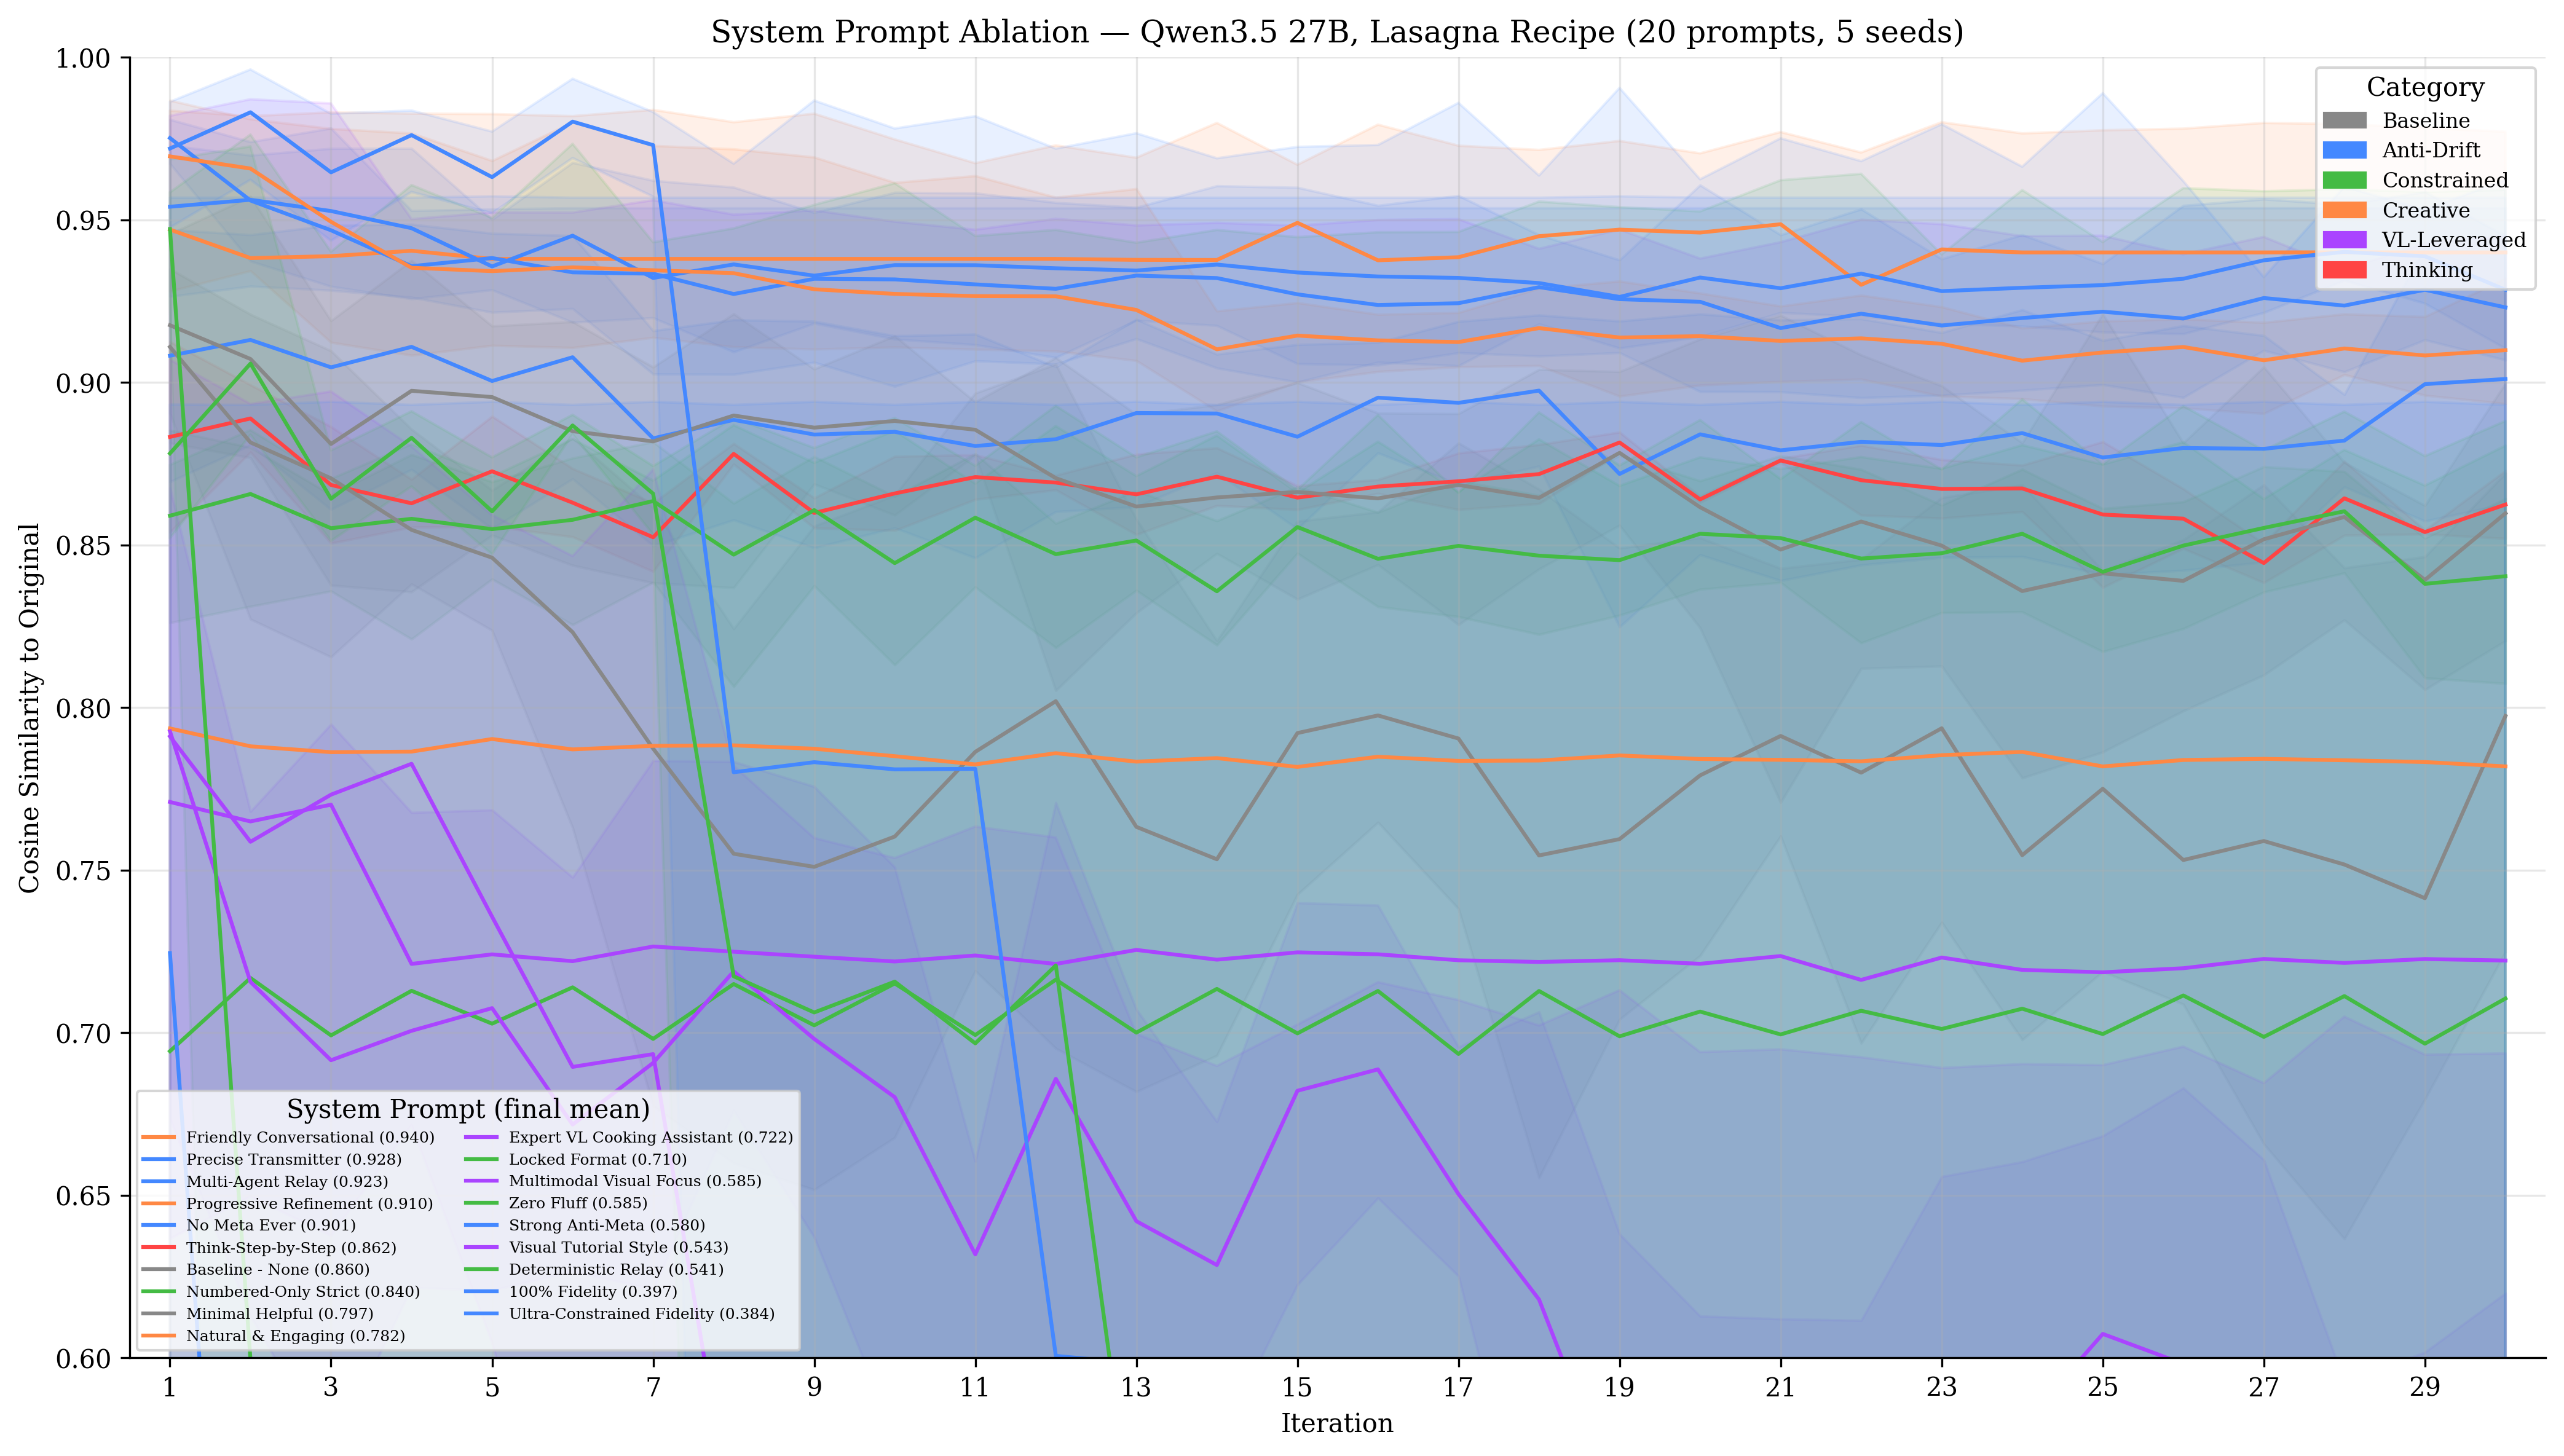
\includegraphics[width=\textwidth,height=0.31\textheight,keepaspectratio]{../results/qwen35_paper_figures/fig7_sysprompt_hero.png}
\caption{System prompt ablation on Qwen3.5 27B GGUF, lasagna recipe.
  20 prompts shown with mean $\pm$ min/max band over the completed chains
  for each prompt. Prompts 15--20 rest on fewer than 5 chains and
  ``Balanced Clarity'' on none (Section~\ref{sec:design}).}
\label{fig:q35_syshero}
\end{figure}

\begin{figure}[htbp]
  \centering
  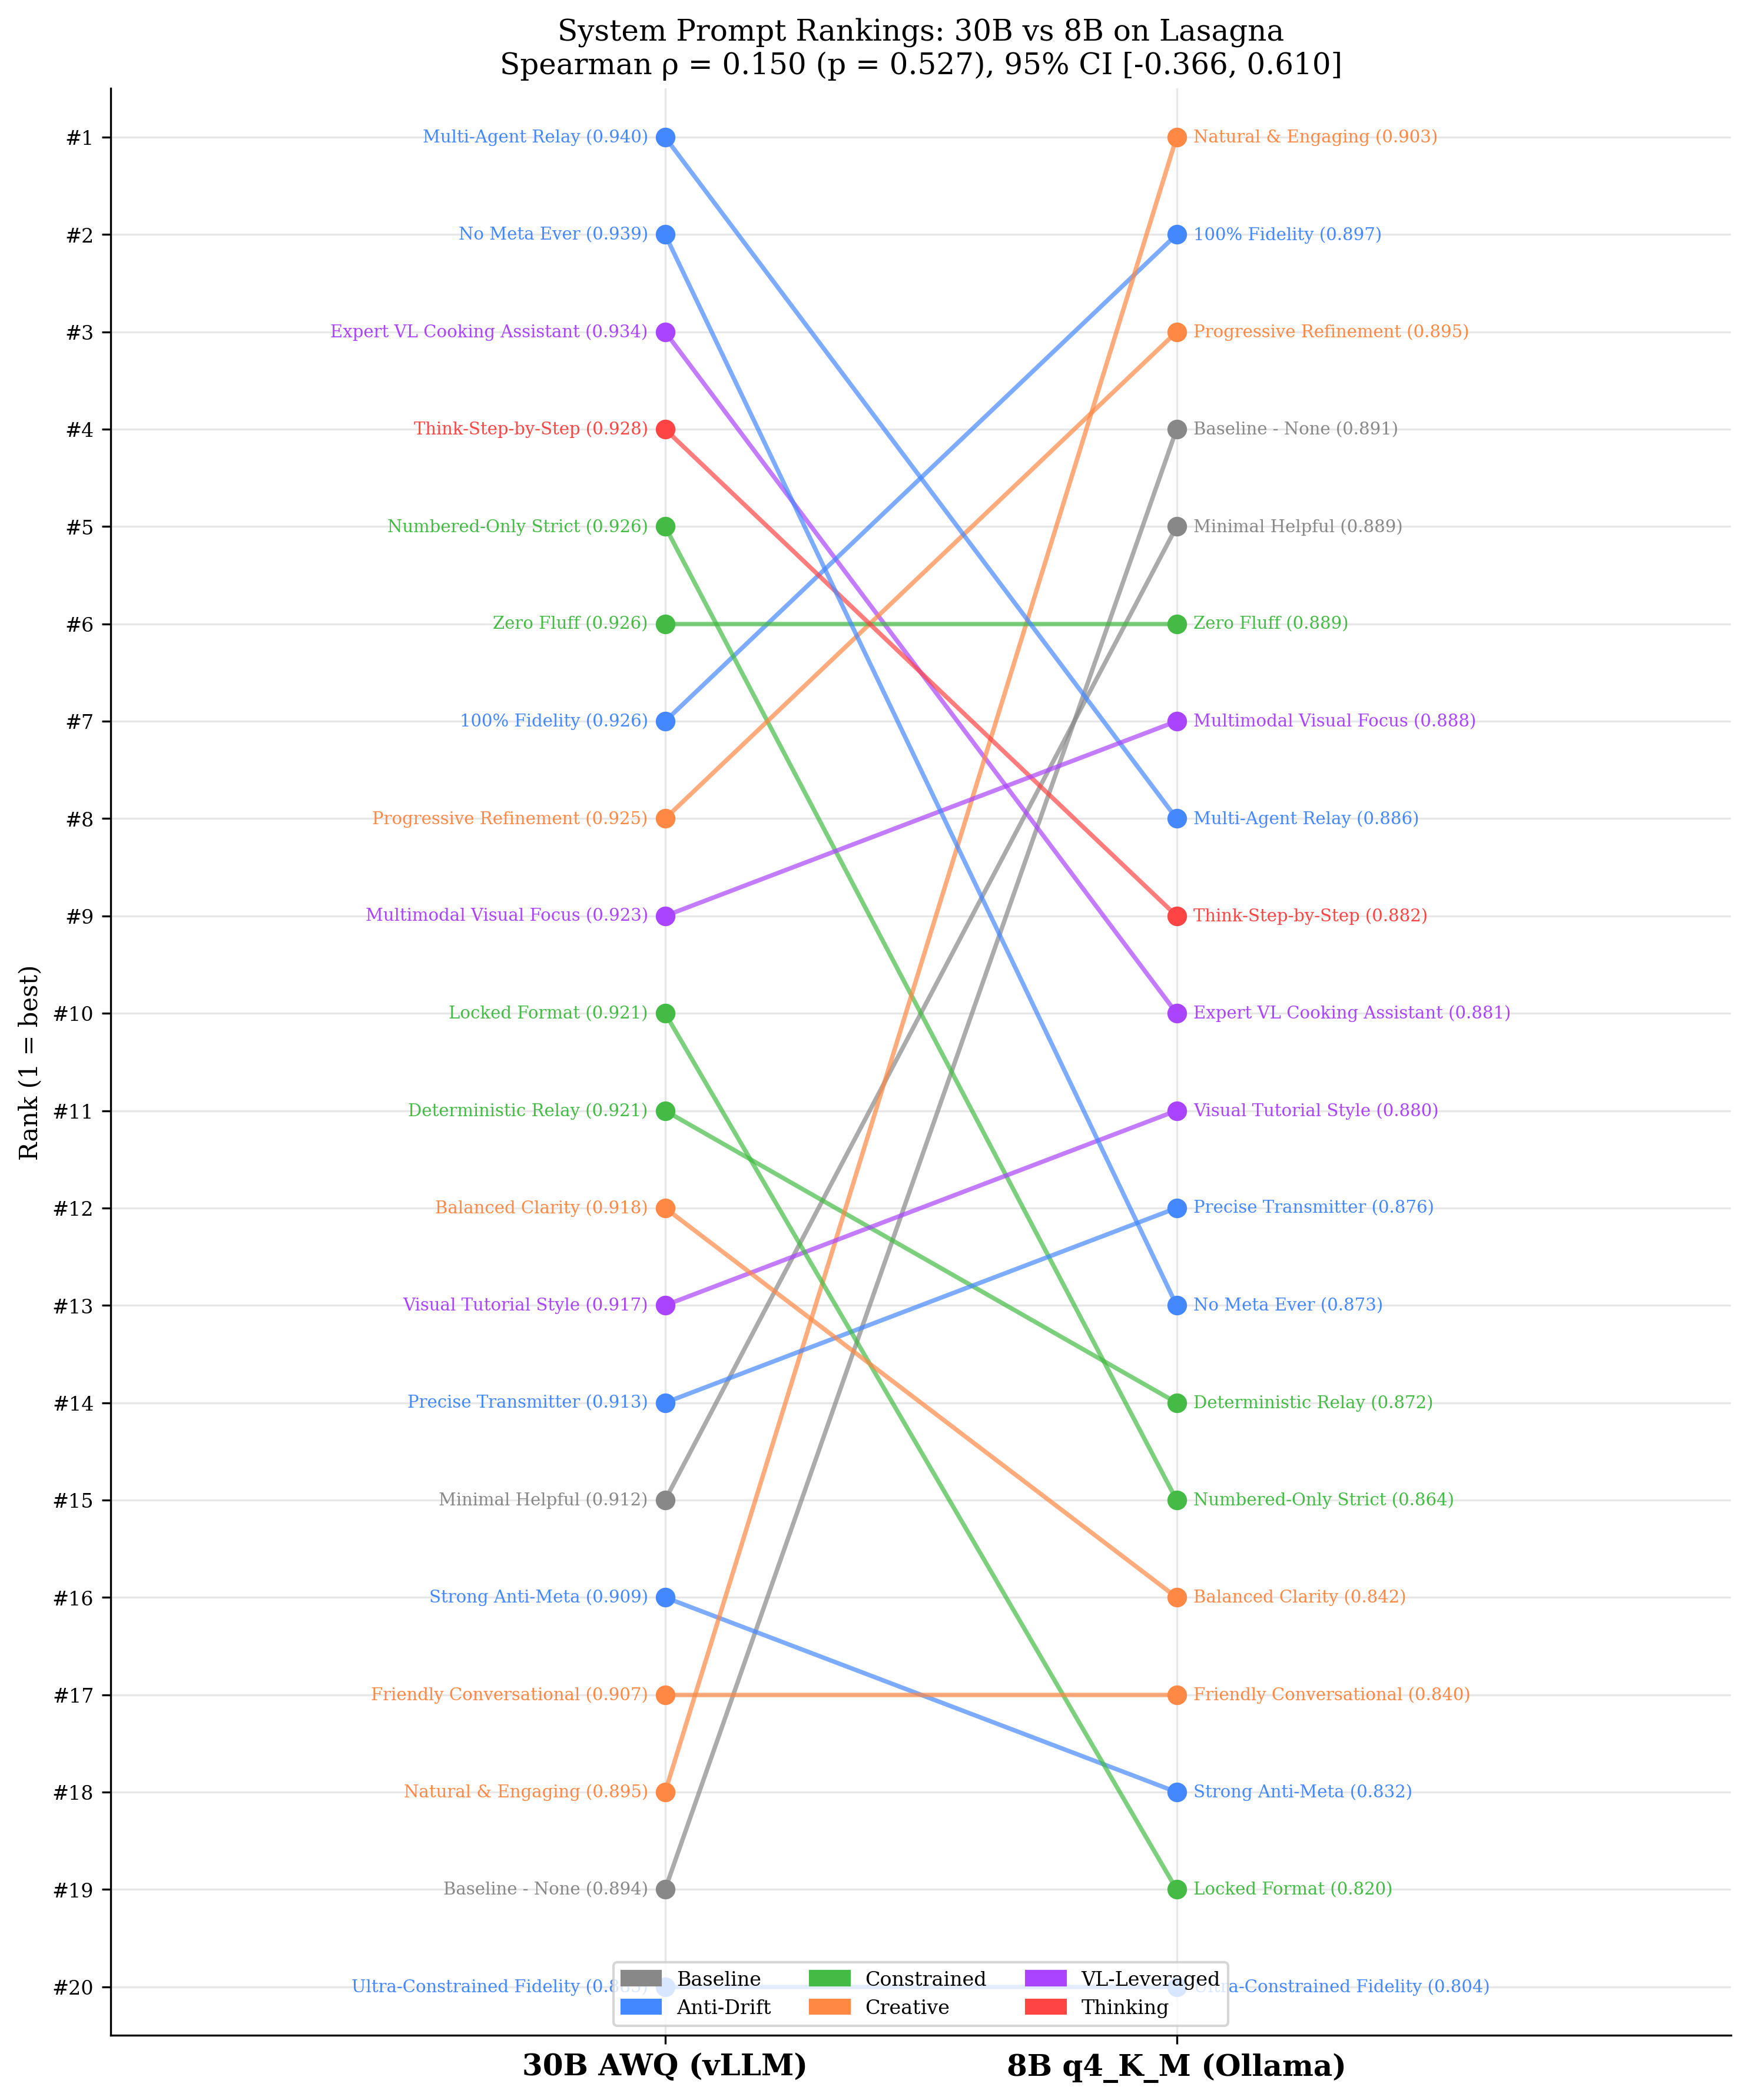
\includegraphics[width=\textwidth,height=0.31\textheight,keepaspectratio]{../results/paper_figures/fig7_cross_model.png}
  \caption{System prompt rankings are uncorrelated across model sizes.
  Slopes show rank changes between 30B (left) and 8B (right) on lasagna.}
  \label{fig:cross_model}
\end{figure}

\begin{figure}[htbp]
\centering
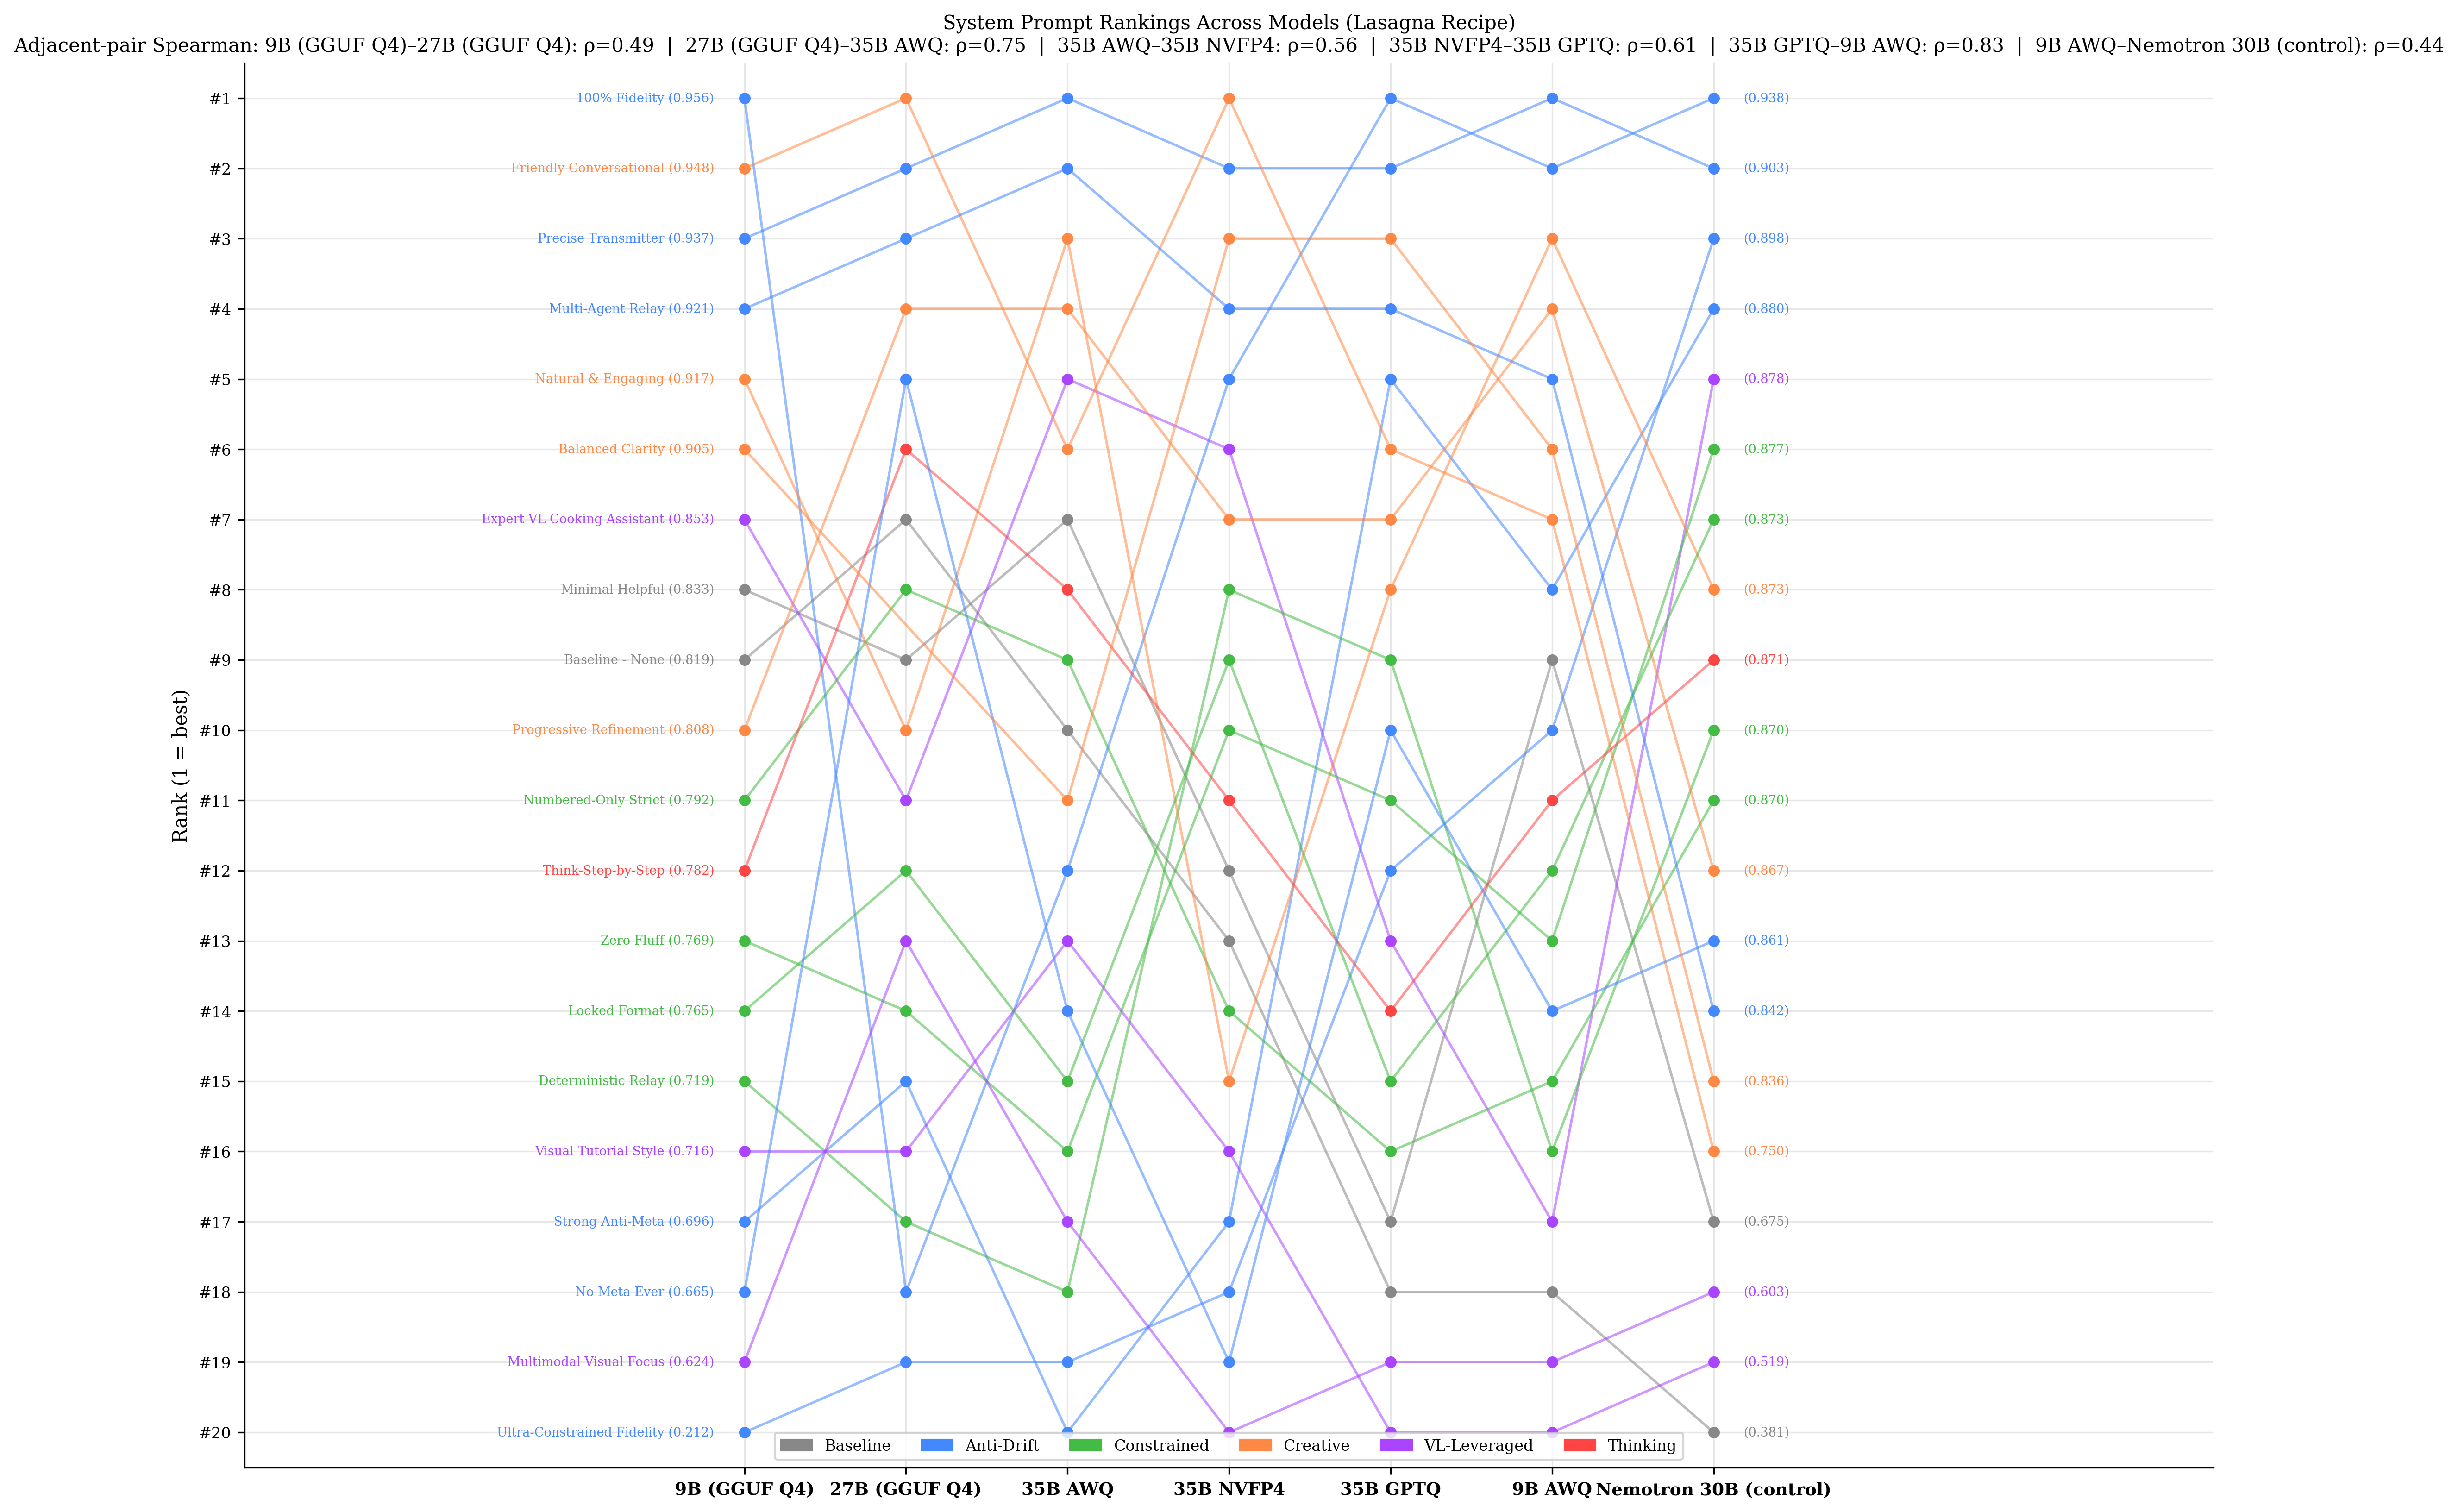
\includegraphics[width=\textwidth,height=0.31\textheight,keepaspectratio]{../results/qwen35_paper_figures/fig8_sysprompt_cross_model.png}
\caption{System prompt rankings across all six Qwen3.5 configurations and
  the Nemotron control (lasagna). Adjacent-column Spearman $\rho$ values
  are annotated; the full matrix with bootstrap CIs is in
  Table~\ref{tab:rq4_spread}.}
\label{fig:q35_syscross}
\end{figure}

\begin{figure}[htbp]
  \centering
  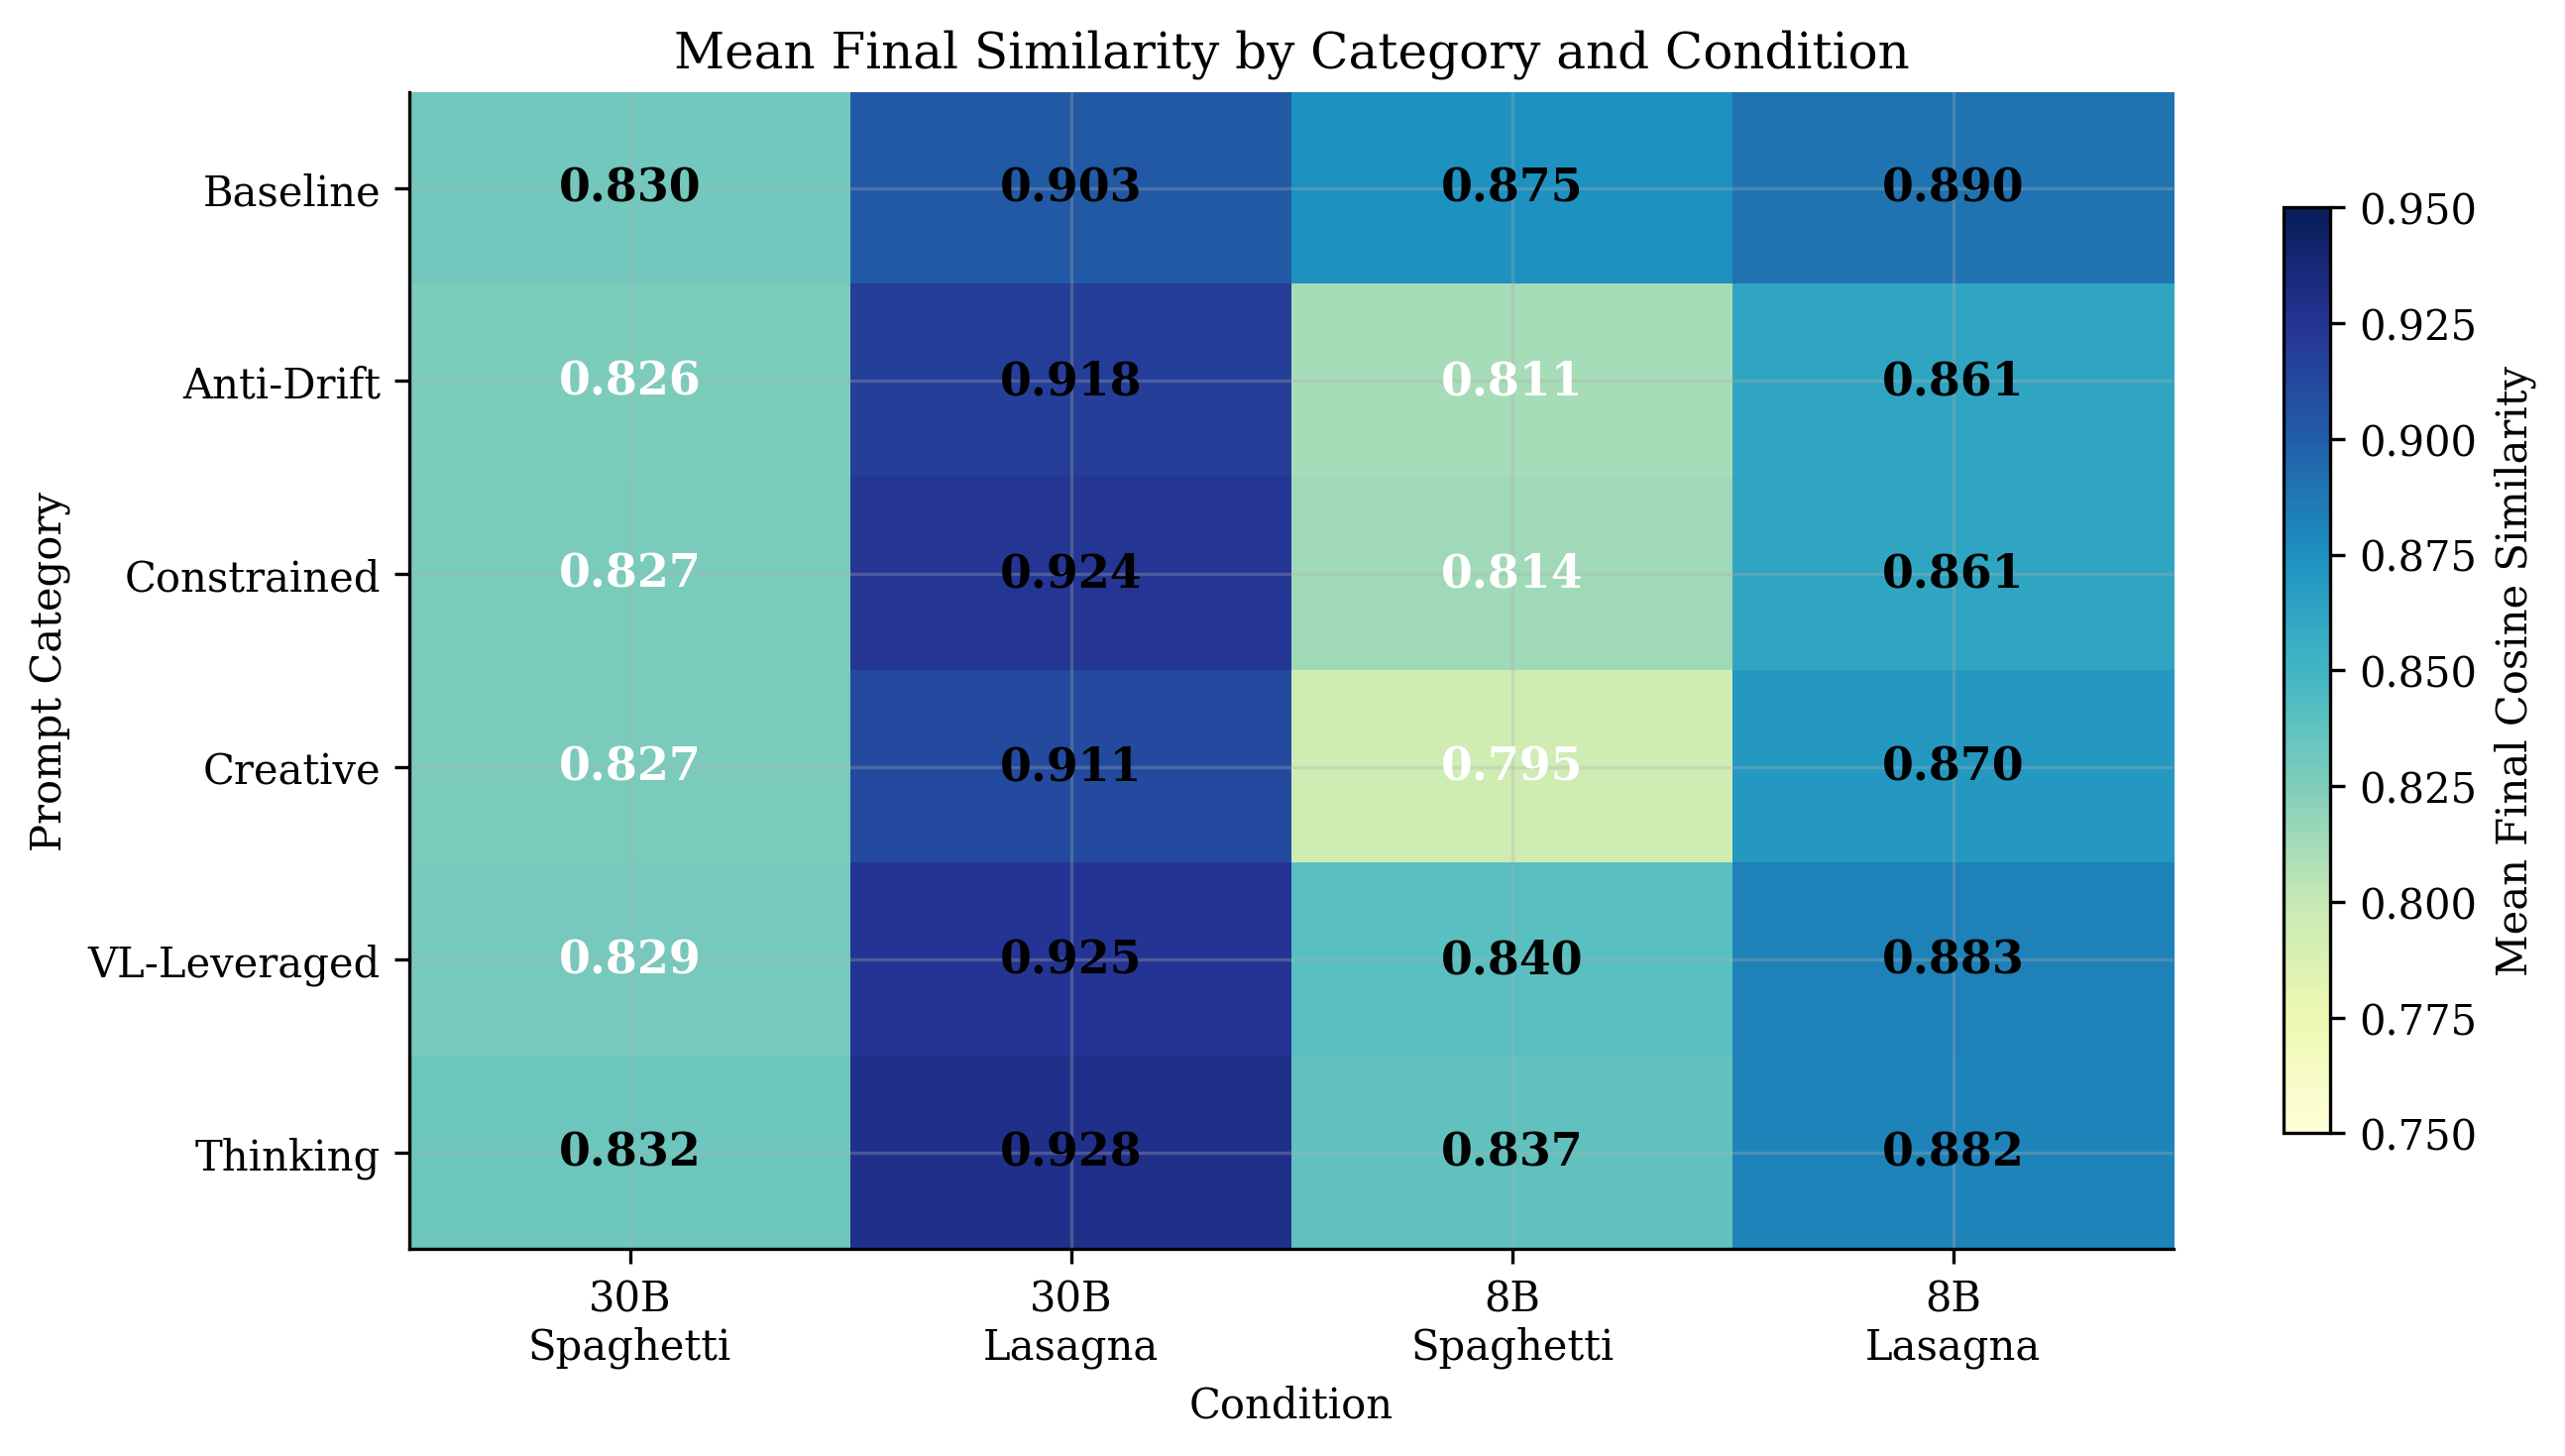
\includegraphics[width=\textwidth,height=0.31\textheight,keepaspectratio]{../results/paper_figures/fig8_category_heatmap.png}
  \caption{Mean final similarity by prompt category and cross-family condition.}
  \label{fig:category_heatmap}
\end{figure}

\begin{figure}[htbp]
\centering
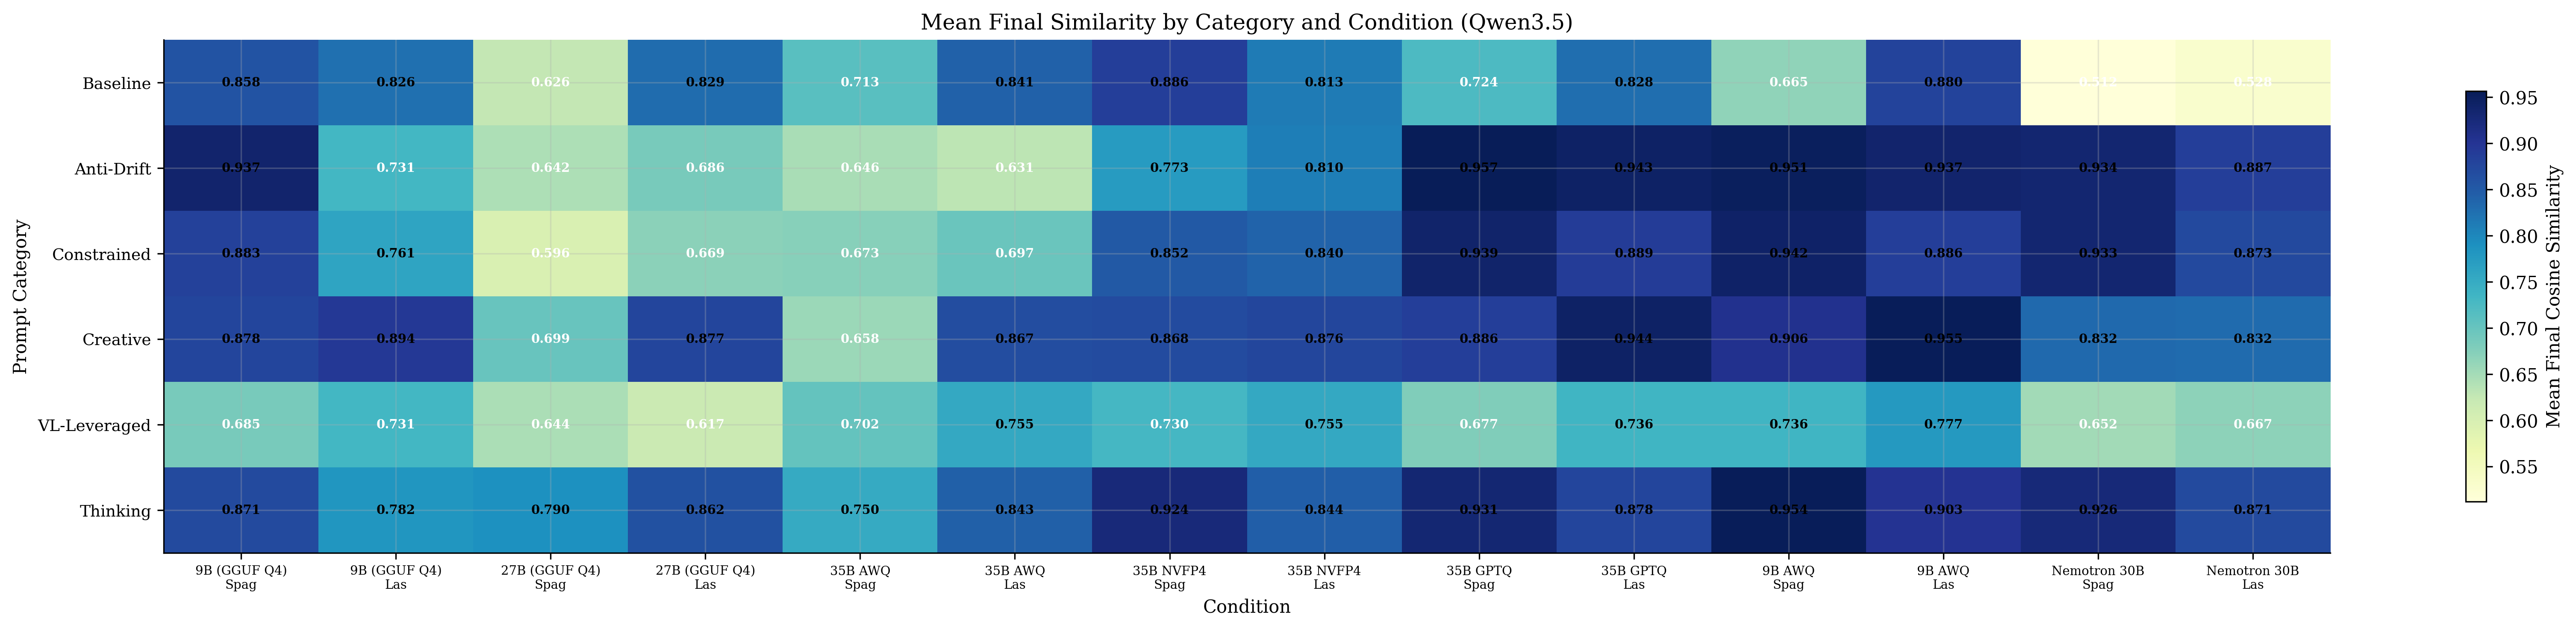
\includegraphics[width=\textwidth,height=0.31\textheight,keepaspectratio]{../results/qwen35_paper_figures/fig9_category_heatmap.png}
\caption{Mean final similarity by prompt category and Qwen3.5 condition.}
\label{fig:q35_catheat}
\end{figure}

\begin{table}[t]
\centering
\caption{RQ4 summary (lasagna recipe), computed over \emph{clean}
  chains only. Spread is the difference between the best- and
  worst-performing system prompt for that configuration;
  $n_{\min}$ is the smallest number of clean chains behind any
  prompt cell; ``RA'' is the configuration-wide runaway-thinking rate
  over all 20 prompts $\times$ 5 seeds.}
\label{tab:rq4_spread}
\small
\resizebox{\textwidth}{!}{%
\begin{tabular}{lccllcc}
\toprule
Configuration & Mean & Spread & Best prompt & Worst prompt & $n_{\min}$ & RA \\
\midrule
9B (GGUF Q4) & 0.822 & 0.332 & 100\% Fidelity (0.956) & Multimodal Visual Focus (0.624) & 1 & 0.05 (5/97) \\
27B (GGUF Q4) & 0.868 & 0.380 & Natural \& Engaging (0.965) & Multimodal Visual Focus (0.585) & 1 & 0.20 (16/81) \\
35B AWQ & 0.742 & 0.743 & Precise Transmitter (0.917) & Strong Anti-Meta (0.175) & 5 & 0.00 (0/100) \\
35B NVFP4 & 0.854 & 0.294 & Balanced Clarity (0.956) & Multimodal Visual Focus (0.663) & 2 & 0.30 (30/99) \\
35B GPTQ & 0.887 & 0.348 & 100\% Fidelity (0.981) & Visual Tutorial Style (0.633) & 4 & 0.00 (0/99) \\
9B AWQ & 0.899 & 0.300 & Precise Transmitter (0.972) & Visual Tutorial Style (0.672) & 4 & 0.00 (0/99) \\
Nemotron 30B (control) & 0.803 & 0.556 & 100\% Fidelity (0.938) & Baseline - None (0.381) & 5 & 0.00 (0/100) \\
\bottomrule
\end{tabular}}

\vspace{1em}

\caption*{Pairwise Spearman $\rho$ between per-prompt mean rankings
  (20 prompts, lasagna), with 95\% bootstrap CIs ($B=10{,}000$).}
\small
\begin{tabular}{llcc}
\toprule
Configuration A & Configuration B & $\rho$ & 95\% CI \\
\midrule
9B (GGUF Q4) & 27B (GGUF Q4) & 0.486 & [-0.075, 0.897] \\
9B (GGUF Q4) & 35B AWQ & 0.779 & [0.461, 0.918] \\
9B (GGUF Q4) & 35B NVFP4 & 0.798 & [0.444, 0.944] \\
9B (GGUF Q4) & 35B GPTQ & 0.549 & [0.070, 0.825] \\
9B (GGUF Q4) & 9B AWQ & 0.633 & [0.209, 0.857] \\
9B (GGUF Q4) & Nemotron 30B (control) & 0.081 & [-0.488, 0.573] \\
27B (GGUF Q4) & 35B AWQ & 0.746 & [0.420, 0.897] \\
27B (GGUF Q4) & 35B NVFP4 & 0.409 & [-0.171, 0.819] \\
27B (GGUF Q4) & 35B GPTQ & 0.209 & [-0.326, 0.707] \\
27B (GGUF Q4) & 9B AWQ & 0.312 & [-0.202, 0.714] \\
27B (GGUF Q4) & Nemotron 30B (control) & -0.333 & [-0.781, 0.204] \\
35B AWQ & 35B NVFP4 & 0.556 & [0.123, 0.800] \\
35B AWQ & 35B GPTQ & 0.259 & [-0.200, 0.644] \\
35B AWQ & 9B AWQ & 0.480 & [0.012, 0.794] \\
35B AWQ & Nemotron 30B (control) & -0.093 & [-0.560, 0.390] \\
35B NVFP4 & 35B GPTQ & 0.611 & [0.180, 0.855] \\
35B NVFP4 & 9B AWQ & 0.523 & [0.080, 0.785] \\
35B NVFP4 & Nemotron 30B (control) & 0.162 & [-0.369, 0.618] \\
35B GPTQ & 9B AWQ & 0.829 & [0.542, 0.937] \\
35B GPTQ & Nemotron 30B (control) & 0.496 & [-0.060, 0.839] \\
9B AWQ & Nemotron 30B (control) & 0.441 & [-0.071, 0.784] \\
\bottomrule
\end{tabular}
\end{table}


\begin{table}[t]
\centering
\caption{System prompt effects on the lasagna recipe across all tested
  Qwen3.5 configurations plus the out-of-family Nemotron control. Mean
  final cosine similarity over the \emph{clean} chains for that cell
  (chains containing no empty, runaway-thinking generation; up to 5 per
  cell). A superscript gives $n_c$ when fewer than 5 clean chains
  survive; ``---'' marks a cell with no clean chain at all. The last two
  rows give the smallest per-cell $n_c$ and the configuration-wide
  runaway-thinking rate. Sorted by the mean across configurations.}
\label{tab:sysprompt}
\scriptsize
\resizebox{\textwidth}{!}{%
\begin{tabular}{llcccccccc}
\toprule
Prompt & Category & 9B (GGUF Q4) & 27B (GGUF Q4) & 35B AWQ & 35B NVFP4 & 35B GPTQ & 9B AWQ & Nemotron 30B & Mean \\
\midrule
Precise Transmitter & Anti-Drift & 0.937 & 0.928 & 0.917 & 0.941 & 0.976 & 0.972$^{4}$ & 0.903 & 0.939 \\
Natural \& Engaging & Creative & 0.917 & 0.965$^{4}$ & 0.914 & 0.929$^{4}$ & 0.932 & 0.968 & 0.873 & 0.928 \\
100\% Fidelity & Anti-Drift & 0.956$^{4}$ & 0.917$^{2}$ & 0.806 & 0.881$^{4}$ & 0.981 & 0.970 & 0.938 & 0.921 \\
Multi-Agent Relay & Anti-Drift & 0.921 & 0.923$^{3}$ & 0.915 & 0.917$^{4}$ & 0.959 & 0.964 & 0.842 & 0.920 \\
Balanced Clarity & Creative & 0.905$^{3}$ & --- & 0.810 & 0.956$^{3}$ & 0.969 & 0.959 & 0.836 & 0.906 \\
Friendly Conversational & Creative & 0.948 & 0.940$^{1}$ & 0.869 & 0.953$^{4}$ & 0.940 & 0.924 & 0.750 & 0.903 \\
Progressive Refinement & Creative & 0.808 & 0.910 & 0.876 & 0.863 & 0.936 & 0.967 & 0.867 & 0.890 \\
Expert VL Cooking Assistant & VL-Leveraged & 0.853 & 0.890$^{4}$ & 0.872 & 0.869 & 0.881 & 0.865 & 0.878 & 0.873 \\
Think-Step-by-Step & Thinking & 0.782 & 0.862$^{2}$ & 0.843 & 0.844 & 0.878 & 0.903 & 0.871 & 0.855 \\
Numbered-Only Strict & Constrained & 0.792 & 0.840 & 0.842 & 0.811$^{4}$ & 0.872 & 0.881 & 0.870 & 0.844 \\
Zero Fluff & Constrained & 0.769 & 0.941$^{3}$ & 0.660 & 0.854$^{3}$ & 0.903 & 0.893 & 0.877 & 0.842 \\
Locked Format & Constrained & 0.765 & 0.875$^{4}$ & 0.745 & 0.846$^{2}$ & 0.874 & 0.893 & 0.873 & 0.839 \\
No Meta Ever & Anti-Drift & 0.665 & 0.901$^{2}$ & 0.746 & 0.841$^{3}$ & 0.907 & 0.884 & 0.861 & 0.829 \\
Minimal Helpful & Baseline & 0.833 & 0.797 & 0.859 & 0.814 & 0.832 & 0.909 & 0.675 & 0.817 \\
Deterministic Relay & Constrained & 0.719 & 0.868$^{3}$ & 0.542 & 0.861$^{2}$ & 0.907 & 0.875 & 0.870 & 0.806 \\
Strong Anti-Meta & Anti-Drift & 0.857$^{4}$ & 0.934$^{3}$ & 0.175 & --- & 0.943 & 0.924 & 0.880 & 0.786 \\
Ultra-Constrained Fidelity & Anti-Drift & 0.858$^{1}$ & 0.886$^{2}$ & 0.228 & --- & 0.892 & 0.907 & 0.898 & 0.778 \\
Baseline - None & Baseline & 0.819 & 0.860 & 0.822 & 0.813$^{4}$ & 0.823 & 0.851 & 0.381 & 0.767 \\
Visual Tutorial Style & VL-Leveraged & 0.716 & 0.666$^{4}$ & 0.766 & 0.710$^{4}$ & 0.633 & 0.672 & 0.519 & 0.669 \\
Multimodal Visual Focus & VL-Leveraged & 0.624 & 0.585$^{3}$ & 0.626 & 0.663$^{3}$ & 0.694$^{4}$ & 0.795 & 0.603 & 0.656 \\
\midrule
\multicolumn{2}{l}{Minimum $n_c$} & 1 & 0 & 5 & 0 & 4 & 4 & 5 & \\
\multicolumn{2}{l}{Runaway rate} & 0.05 & 0.20 & 0.00 & 0.30 & 0.00 & 0.00 & 0.00 & \\
\bottomrule
\end{tabular}}
\end{table}


\paragraph{The complexity threshold is a property of the model, not of the
task.}
On the cross-family 30B AWQ model the 20 prompts are indistinguishable on the
3-step recipe (spread 0.008) and separate only on the 21-step recipe (spread
0.054), the pattern Figure~\ref{fig:complexity} shows. On the cross-family
8B model the spreads are 0.154 and 0.098, and within the Qwen3.5 family they
are larger still and no longer ordered by recipe: 0.30--0.49 on spaghetti and
0.29--0.74 on lasagna across the six configurations
(Table~\ref{tab:rq4_spread}), with the Nemotron control at 0.50 and 0.56.
The threshold therefore describes a model that is already near its ceiling,
where no prompt can help and only a long input gives one room to hurt. For a
configuration that drifts on its own, prompts matter on any input.

\paragraph{Which prompts help, and which break the model.}
Where prompts matter, the fidelity-oriented prompts win: 100\% Fidelity,
Precise Transmitter and Ultra-Constrained Fidelity take the best position on
nine of the twelve Qwen3.5 configuration--recipe pairs, reaching
0.96--0.99, and the visually oriented prompts (Visual Tutorial Style,
Multimodal Visual Focus) take the worst position on nine of the twelve, at 0.59--0.67,
below the no-prompt baseline. The cross-family 30B AWQ model is the
exception in both directions: its best prompts are the anti-meta-commentary
ones (Multi-Agent Relay, No Meta Ever) and Ultra-Constrained Fidelity is its
worst. That prompt is also the one that most reliably triggers runaway
thinking on the reasoning-enabled builds (Section~\ref{sec:runaway}): it is
the best prompt on the 35B GPTQ-Int4 and 9B AWQ builds served by vLLM and a
guaranteed failure on the 35B NVFP4 build served by SGLang. The same words
are the best or the worst instruction depending on the stack they run on.

\paragraph{Rankings transfer between related configurations only.}
Across families, prompt rankings on 30B AWQ and 8B q4\_K\_M are uncorrelated
(Spearman $\rho = 0.15$, $p = 0.53$, 95\% CI $[-0.37, 0.61]$;
Figure~\ref{fig:cross_model}). Within the Qwen3.5 family the picture is
graded rather than binary (Table~\ref{tab:rq4_spread},
Figure~\ref{fig:q35_syscross}). The strongest agreement is between the two
vLLM builds of different sizes, 35B GPTQ-Int4 and 9B AWQ ($\rho = 0.83$, CI
[0.54, 0.94]), and between the 9B GGUF build and the two 35B non-GGUF builds
(0.78 and 0.80). Agreement between formats of the same 35B checkpoint is
weaker (AWQ--GPTQ 0.26, AWQ--NVFP4 0.56, NVFP4--GPTQ 0.61), and between the
two GGUF sizes weaker still (9B--27B 0.49). Every correlation with the
out-of-family Nemotron control is weak ($-0.33$ to $0.50$) and every one of
those intervals includes zero. Prompt
rankings, then, are neither universal nor arbitrary: they are shared by
configurations that share a serving stack and a family, and they do not
survive a change of family. Table~\ref{tab:sysprompt} gives the per-prompt
means and Figures~\ref{fig:category_heatmap} and~\ref{fig:q35_catheat} the
category view, in which the VL-Leveraged category is the worst on every one
of the fourteen within-family columns.


\clearpage
\subsection{Embedding Model Validation}
\label{sec:embedding}

To validate that our results are not an artifact of the embedding model, we
re-embedded all saved texts with bge-m3~\citep{chen2024bgem3} in addition to
the primary Qwen3-Embedding-0.6B~\citep{zhang2025qwen3embedding}, separately
for each dataset.

On the cross-family data (Figure~\ref{fig:embedding}), the Pearson correlation
is $r = 0.960$ and Spearman $\rho = 0.857$ ($n = 21{,}636$ pairs, both
$p < 10^{-10}$).

On the within-family data, 20{,}072 of 22{,}167 pairs (90.6\%) produced valid
similarities from both models, yielding $r = 0.825$ and $\rho = 0.815$
($p < 10^{-10}$ for both). The remaining 2{,}095 pairs (9.4\%) failed because
bge-m3's serving endpoint rejects inputs exceeding its 8{,}192-token context
window rather than truncating them, whereas Qwen3-Embedding-0.6B accepts
32{,}768 tokens. All failed pairs are outputs exceeding 6{,}000 words, produced
by the runaway text expansion described in Section~\ref{sec:runaway}; their mean
Qwen similarity is 0.515 (median 0.572) against a dataset mean of 0.829,
confirming that they are systematically the most-drifted outputs. Because both
embedding models would score these highly-diverged texts as low similarity,
their exclusion is unlikely to meaningfully affect the correlation. Details are
in Appendix~\ref{app:embedding}.

\begin{figure}[htbp]
  \centering
  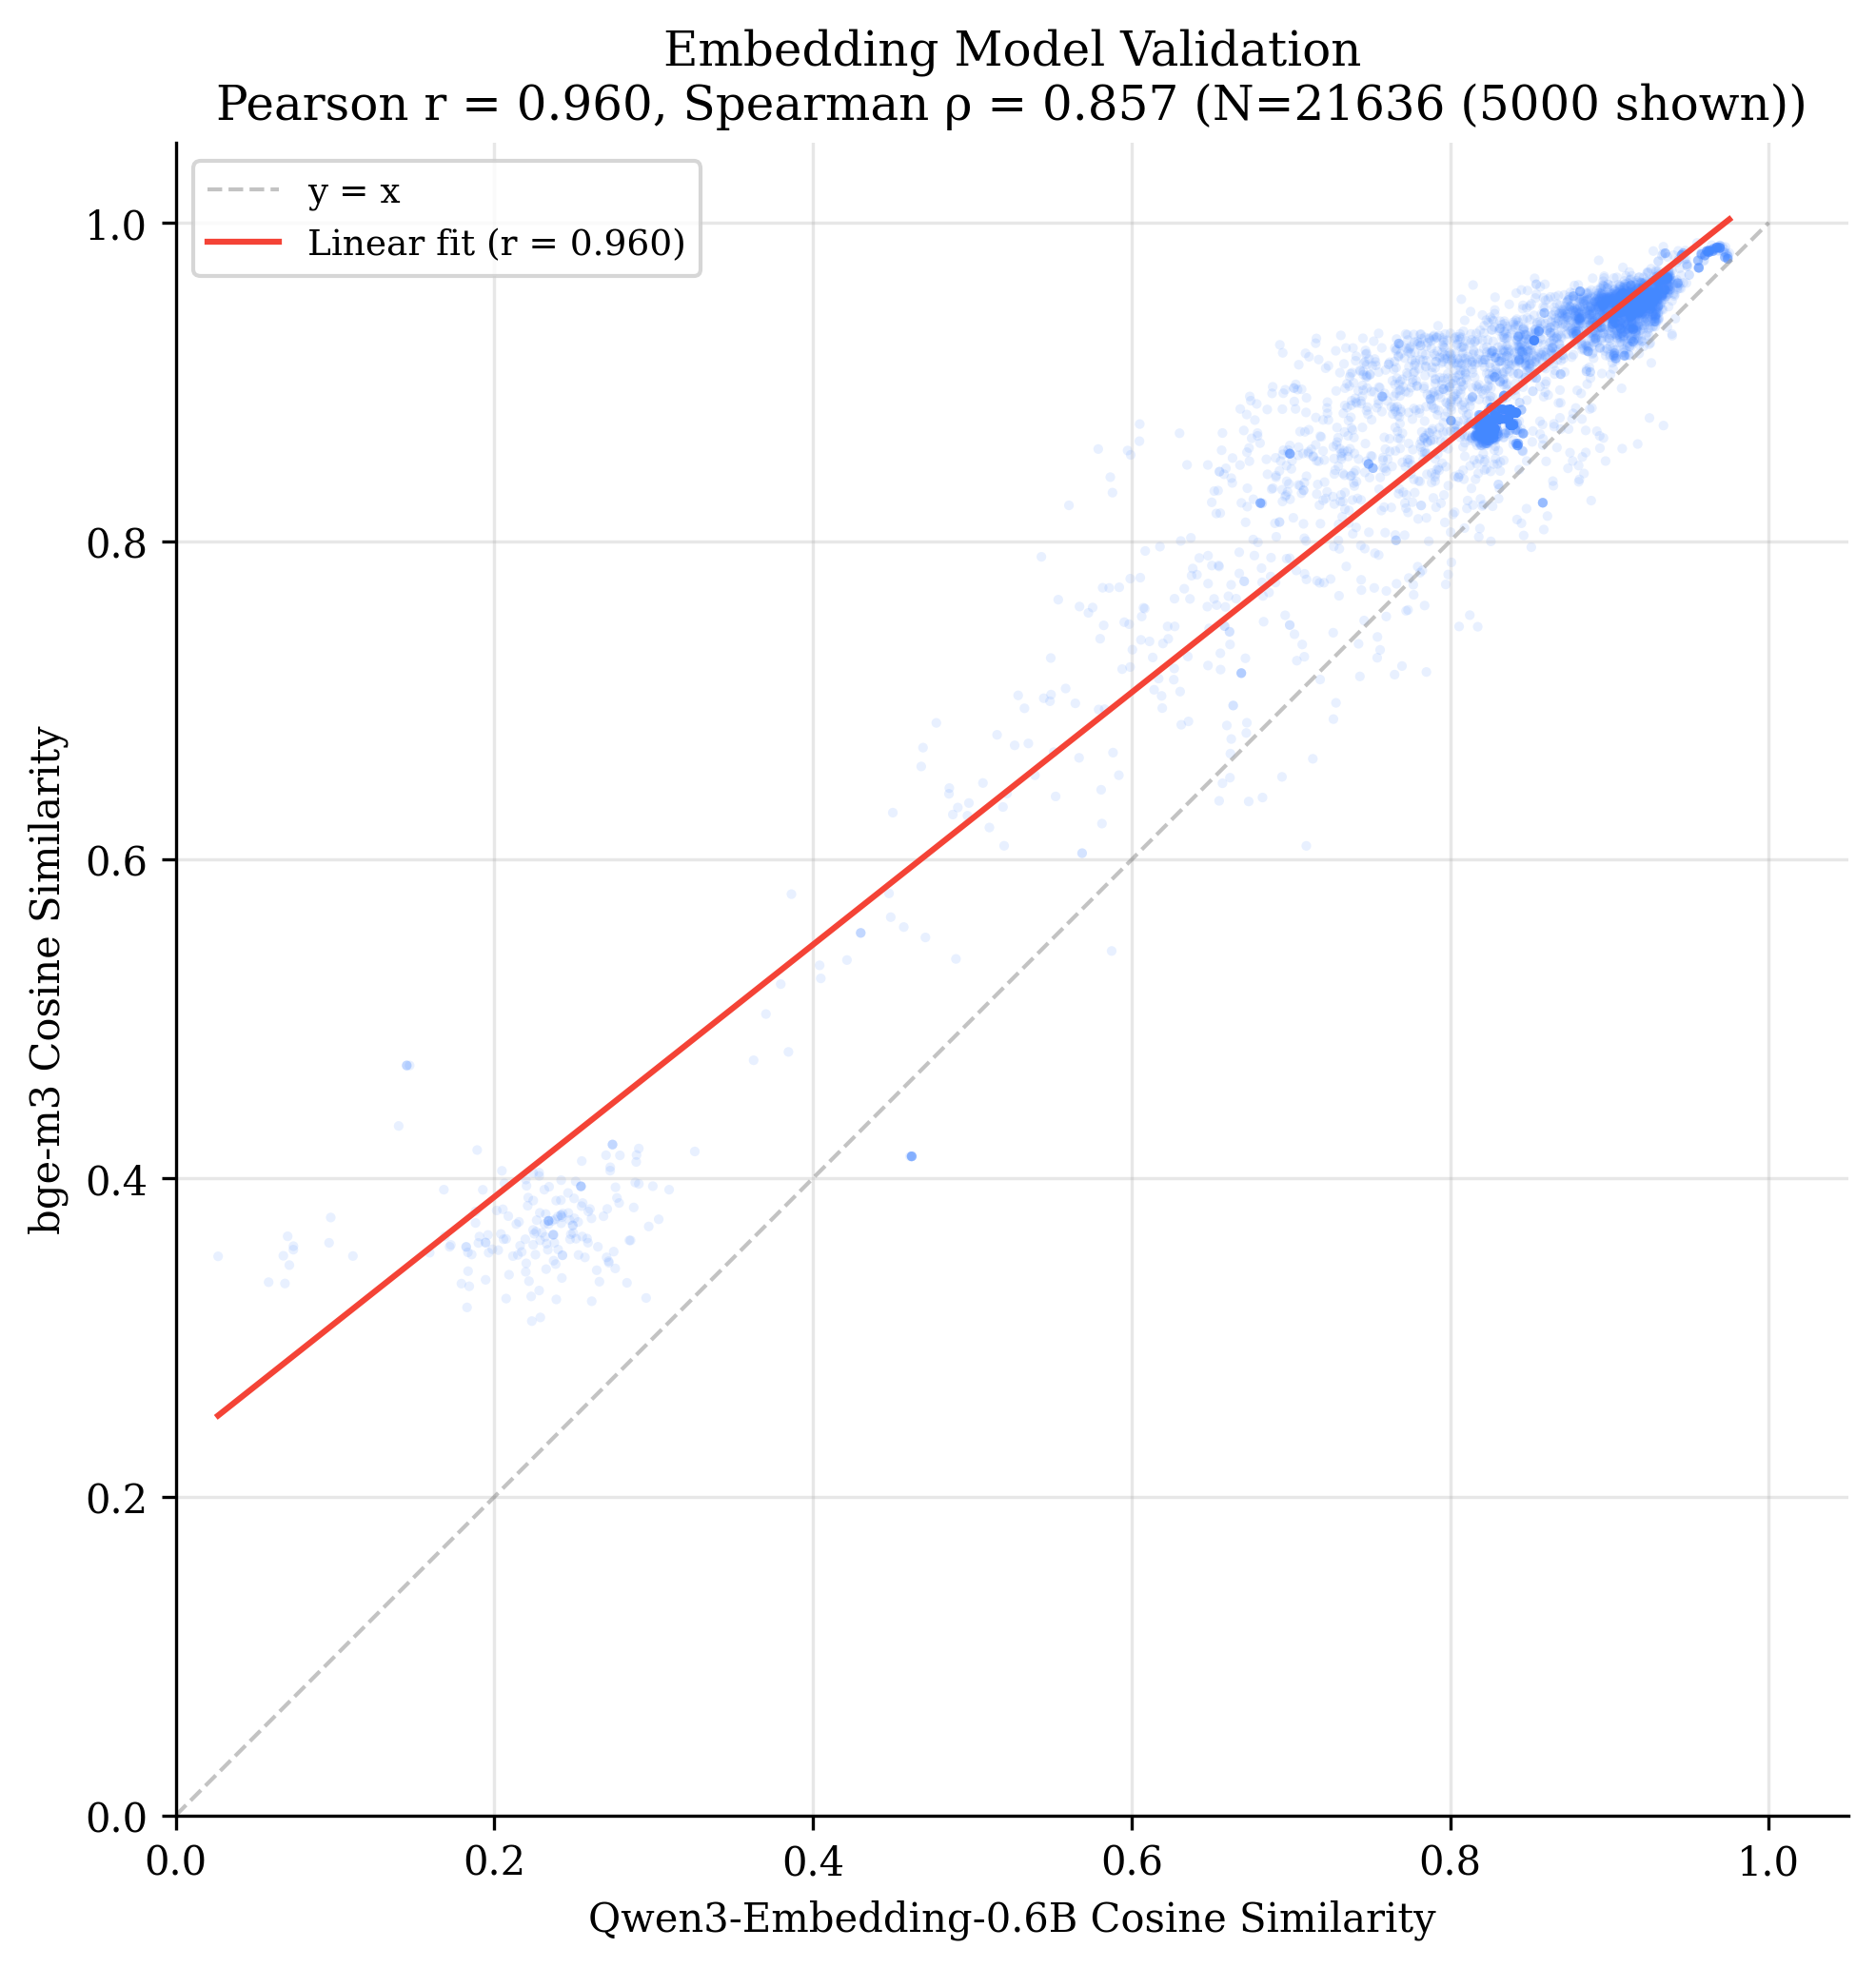
\includegraphics[width=\textwidth,height=0.31\textheight,keepaspectratio]{../results/paper_figures/fig10_embedding_scatter.png}
  \caption{Embedding model validation on the cross-family data: cosine
  similarity scores from Qwen3-Embedding-0.6B vs.\ bge-m3 across all
  experimental conditions.}
  \label{fig:embedding}
\end{figure}

% ═══════════════════════════════════════════════════════════════════════════════
% 5. DISCUSSION
% ═══════════════════════════════════════════════════════════════════════════════

\clearpage
\section{Discussion}
\label{sec:discussion}

\paragraph{Hierarchy of sensitivities.}
Read across the two datasets, the factors governing drift can be ordered by
the size of the effect each produces on final similarity, with one
qualification that the earlier single-dataset ordering did not need. Choice of
model family remains the largest lever: 0.67 separates the best and worst
cross-family models (0.904 vs.\ 0.239, Section~\ref{sec:rq1}). Within a
family, parameter count matters up to the capacity threshold near 4B and
little beyond it: clean-chain means for every configuration above the
threshold lie within 0.10 of one another (Section~\ref{sec:scaling}). The
next rung is not a continuous factor but a failure mode: runaway thinking
removes 0--100\% of a condition's chains depending on stack, precision,
size, stimulus and prompt, and where it occurs it dominates every other
effect (Section~\ref{sec:runaway}). Quantization format follows, at up to
0.26 between 4-bit builds of identical weights on the short stimulus and
under 0.05 on the long one (Section~\ref{sec:quantformat}). Temperature and
KV-cache precision are the smallest continuous factors for stable
configurations---within 0.06 across the temperature range for the stable
cross-family models, and KV deltas of $-0.10$ to $+0.26$ of which eight of
ten have intervals including zero---but both grow large below the threshold,
where temperature sensitivity inverts (Sections~\ref{sec:rq2}
and~\ref{sec:temperature}). System prompts are the qualification. On the most
stable model they are the smallest factor of all (spread 0.008 on the short
recipe, 0.054 on the long one), which is the ordering the cross-family
dataset alone suggests; on every within-family configuration they are among
the largest, with spreads of 0.3--0.7 and individual prompts able to trigger
runaway in every chain. The prompt effect is thus not a fixed rung but a
multiplier on how far a configuration already drifts. The practical reading
is unchanged in direction and sharpened in emphasis: choose the model
family first, stay above the capacity threshold, benchmark the exact
quantized build on the exact stack, check explicitly for runaway and empty
completions, and only then tune prompts---knowing that a prompt tuned on one
build may be the worst choice on another.

\paragraph{Fixed-point attractors.}
We observe that a substantial fraction of runs converge to fixed points where
similarity remains constant for 10+ consecutive iterations. This is consistent
with the iterated function system formalization of \citet{chytas2025concept}
and the attractor cycle dynamics of \citet{wang2025attractor}. Models with
strong instruction-tuning (e.g., qwen3:30b-instruct) appear to have stable
attractors near the original meaning, while weaker models' attractors lie
far from the input distribution. The inverted temperature profiles of
Section~\ref{sec:temperature} are the same phenomenon seen from another angle:
at $T\leq0.3$ several small configurations lock immediately, and added sampling
entropy is what breaks the lock.

\paragraph{Cross-model rank inversion.}
The near-zero Spearman correlation between 30B and 8B prompt rankings
(Section~\ref{sec:rq3}) likely reflects an interaction between prompt complexity
and instruction-following capacity~\citep{jaroslawicz2025ifscale}. The 30B model
has sufficient capacity to simultaneously obey negative constraints (``never
reference the chain'') and paraphrase faithfully, so anti-drift prompts excel.
The 8B model, with less headroom, appears to trade off constraint adherence
against paraphrase quality: lightweight prompts like Natural \& Engaging
outperform because they do not compete for the model's limited
instruction-following bandwidth. The within-family results show that this is not
only a size effect: rankings also diverge between quantization formats of the
same checkpoint, where capacity is nominally unchanged.

\paragraph{Non-monotonic precision effects.}
The finding that fp16 KV cache can \emph{worsen} drift in some models, and that
BF16 weights can lose to Q8\_0 or Q4\_K\_M at the same size, challenges the
assumption that higher precision is always better for sequential
generation. We hypothesize that quantization noise can act as a
beneficial regularizer, preventing the model from precisely tracking latent
attractor gradients. This parallels findings in noise injection for optimization
and is consistent with \citet{han2026quantization}'s finding that quantization
errors compound across sequential reasoning steps. At 4-bit, however, the
dominant risk changes character: what limits the Q4\_K\_M configurations is not
gradual fidelity loss but the discrete generation failure of
Section~\ref{sec:runaway}.

\paragraph{Practical recommendations.}
Based on our findings, we offer the following recommendations for multi-agent
LLM system designers:
\begin{enumerate}[leftmargin=*]
  \item \textbf{Model selection is paramount.} Choose instruction-tuned models
        with demonstrated stability; model size alone does not predict drift
        resistance.
  \item \textbf{Stay above the capacity threshold.} Models below roughly 4B
        parameters are unreliable for iterated tasks regardless of
        quantization.
  \item \textbf{Benchmark the exact quantized build.} GGUF, AWQ, NVFP4 and
        GPTQ-Int4 are not interchangeable for drift-sensitive applications
        even at identical nominal precision; test all candidate formats on
        representative tasks.
  \item \textbf{Profile KV cache effects.} Do not assume fp16 KV is always
        better; test with your specific model and quantization combination.
  \item \textbf{Test at operating temperature.} Drift behavior changes
        non-linearly with temperature, and the direction of the effect inverts
        below the stability threshold; validate at the exact temperature used
        in production.
  \item \textbf{Monitor for empty and runaway outputs explicitly.} Aggregate
        similarity scores hide the discrete failure modes of
        Section~\ref{sec:runaway}; check for empty completions and for
        unbounded length growth directly.
  \item \textbf{Prompt complexity matters.} System prompts only help above a
        task complexity threshold; invest in prompt engineering for complex
        pipelines, not simple ones.
  \item \textbf{Prompts don't transfer.} Optimal system prompts are specific to
        the deployed configuration; re-evaluate when changing model, size or
        quantization format.
  \item \textbf{Monitor for tipping points.} Catastrophic drift can occur
        suddenly; implement similarity monitoring with early stopping.
  \item \textbf{Use multiple seeds for evaluation.} Single-run evaluations
        can be misleading; our 8B model shows final similarity ranges of
        0.41--0.92 across seeds for the same prompt.
\end{enumerate}

\paragraph{Limitations.}
\label{sec:limitations}
\begin{itemize}[leftmargin=*]
  \item \textbf{Single domain and single task.} All stimuli are cooking
        recipes and all chains use one paraphrase instruction; other
        domains and other iterated tasks (summarization, translation) may
        drift differently.
  \item \textbf{Serving stacks.} Results cover Ollama, vLLM and SGLang on
        one lab's hardware. In three of the four quantization-format arms the
        format and the backend covary, so the format effect is a
        format-and-stack effect. Runaway thinking was observed only on the
        two stacks that ran Qwen3.5 with reasoning enabled and a
        16{,}384-token budget; a different budget or a stack that disables
        reasoning would change its rate, though not, we expect, its
        existence.
  \item \textbf{Single metric.} Cosine similarity captures one dimension of
        drift. \citet{belem2026certainty} show that repeated rewriting shifts
        expressed certainty while leaving surface content intact, a change
        this metric cannot see; the drift reported here is a lower bound on
        total meaning change, and the validation against a second embedding
        model (Section~\ref{sec:embedding}) bounds only the metric's
        consistency, not its coverage.
  \item \textbf{Seeds are samples, not replicates.} Fixing the sampling seed
        does not pin a chain on these stacks: under batched inference,
        identical seeds produce different trajectories because batch
        composition and kernel scheduling vary between
        requests~\citep{he2025nondeterminism}. Every ``seeded'' run is one
        independent sample, every interval is an interval over those
        samples, and the Kruskal--Wallis and Wilcoxon statistics, which
        treat chains as observations, are reported as descriptive rather
        than inferential.
  \item \textbf{Small $n$ where it matters most.} Several of the sharpest
        contrasts rest on two or three clean chains, because the same
        conditions that separate the formats are the ones that lose chains
        to runaway. The 35B Q4\_K\_M and NVFP4 clean means, in particular,
        should be read as existence results until replicated at higher $n$.
  \item \textbf{The lasagna stimulus is compressed.} The 21-step recipe sent
        to the models collapses steps 12--17 into one line
        (Appendix~\ref{app:prompts}); it is a 16-line stimulus that
        nominally spans 21 steps.
  \item \textbf{Incomplete conditions.} Eleven of the 669 cross-family chains
        and 38 of the 2{,}007 within-family chains did not reach
        iteration~30. They are reported at their actual $n$ or excluded as
        stated in Section~\ref{sec:design}; three of the serving endpoints
        involved have since been retired and those conditions cannot be
        regenerated on the same stack.
  \item \textbf{One out-of-family control.} The Nemotron-3-Nano-30B arm is a
        single model and cannot by itself establish how prompt rankings
        behave across families; it shows only that they need not transfer.
  \item \textbf{No quantization-aware training.} All quantized builds use
        post-training quantization.
\end{itemize}

\paragraph{Future work.}
Extending this framework to non-recipe domains (code generation, legal
documents, medical instructions) would test the generality of the tier
hierarchy and attractor dynamics observed here. Complementary metrics
beyond cosine similarity---such as exact-match entity and quantity tracking,
BERTScore, expressed-certainty measures in the manner of
\citet{belem2026certainty}, or LLM-as-a-judge evaluation for factual
preservation---would capture dimensions of drift (e.g., hallucinated details,
unit substitutions) that embedding-space distance may miss. A companion study
examines the determinism, decoding and cross-generation questions that this one
brackets.

% ═══════════════════════════════════════════════════════════════════════════════
% 6. CONCLUSION
% ═══════════════════════════════════════════════════════════════════════════════
\section{Conclusion}
\label{sec:conclusion}

We presented a systematic study of semantic drift in iterated LLM paraphrase
chains, combining a cross-family sweep of 17 models with a controlled
within-family sweep of the Qwen3.5 family, and isolating model architecture,
scale, quantization level and format, serving infrastructure, temperature and
prompt engineering. Across 2{,}676 chains and roughly 79{,}000 scored
inferences we established that:

\begin{enumerate}[leftmargin=*]
  \item Model family dominates every other factor, producing a stable four-tier
        stability hierarchy with catastrophic tipping-point failures.
  \item Within a family, a stability threshold sits at approximately 4B
        parameters, below which drift behavior becomes unpredictable, and above
        which the ordering by size is irregular.
  \item Quantization effects are non-monotonic and size-dependent, and four
        4-bit formats applied to identical weights produce measurably different
        drift dynamics.
  \item KV cache precision has non-monotonic, directionally mixed effects.
  \item Drift is not reducible to sampling entropy, and temperature sensitivity
        inverts below the stability threshold.
  \item System prompts are effective only above a stimulus complexity
        threshold, and optimal prompts do not transfer across families, sizes,
        or quantization formats.
\end{enumerate}

These findings have immediate implications for the design of reliable multi-agent
LLM systems, where understanding and mitigating semantic drift is essential for
maintaining output quality across sequential processing stages. The interactions
between the factors are complex and non-monotonic, underscoring the need for
empirical benchmarking of the specific model configuration to be deployed rather
than of the family it belongs to.

% ═══════════════════════════════════════════════════════════════════════════════
% REFERENCES
% ═══════════════════════════════════════════════════════════════════════════════
\bibliographystyle{plainnat}
\bibliography{references}

% ═══════════════════════════════════════════════════════════════════════════════
% APPENDICES
% ═══════════════════════════════════════════════════════════════════════════════

\clearpage
\appendix

\section{Prompt Texts}
\label{app:prompts}

\paragraph{Spaghetti (3 steps).}
The stimulus is reproduced verbatim from \texttt{PROMPTS["spaghetti"]} in the
experiment scripts:
\begin{quote}
Step 1: Boil water. Step 2: Add pasta for 8 minutes. Step 3: Drain and serve
with sauce.
\end{quote}

\paragraph{Lasagna (nominally 21 steps).}
The text below is the verbatim stimulus sent to the models
(\texttt{PROMPTS["lasagna"]} in the same scripts). Note that
although the recipe is numbered through step~21, steps 12--17 are compressed
into a single line in the stimulus itself, so the transmitted text contains
16 lines rather than 21. We reproduce it exactly rather than expanding it,
because the compression is part of the condition being measured.
\begin{quote}
\small
Follow these exact steps to prepare a classic homemade beef lasagna that serves
8--10 people:

Step 1: Preheat your oven to 375\textdegree F (190\textdegree C) and lightly
grease a 9$\times$13 inch baking dish.
Step 2: Bring a large pot of lightly salted water to a boil.
Step 3: Heat 2 tablespoons of olive oil in a large skillet over medium heat.
Step 4: Add 1 large finely diced onion and cook for 5 minutes until translucent.
Step 5: Add 5 minced garlic cloves and cook for 1 minute until fragrant.
Step 6: Add 1.25 lbs ground beef and 0.75 lb Italian sausage. Cook until browned.
Step 7: Drain excess grease from the skillet.
Step 8: Stir in two 28-oz cans of crushed tomatoes, 3 tbsp tomato paste, 2 tsp
dried basil, 1.5 tsp dried oregano, 0.5 tsp fennel seed, 1 tsp sugar, 1 tsp salt,
and 0.5 tsp black pepper.
Step 9: Bring to a simmer and cook the meat sauce for 30 minutes.
Step 10: Combine 15 oz ricotta, 1 egg, 1/2 cup Parmesan, 1/4 cup parsley,
1/2 tsp salt, 1/4 tsp pepper.
Step 11: Cook 12 lasagna noodles until al dente. Drain and rinse.
Step 12--17: Layer sauce, noodles, ricotta, mozzarella (3 layers).
Step 18: Cover with foil and bake 25 minutes.
Step 19: Remove foil and bake 25--30 more minutes until golden.
Step 20: Rest 15--20 minutes before slicing.
Step 21: Garnish with fresh basil and serve hot.
\end{quote}

\paragraph{System prompts (20 total).}
The following system prompts span 6 categories: Baseline (2), Anti-Drift (6),
Constrained (4), Creative (4), VL-Leveraged (3), and Thinking (1).

{\small
\begin{description}[style=unboxed,leftmargin=0pt,itemsep=4pt]

\item[\textbf{Baseline}] ~

\textbf{1.\ Baseline -- None.} \emph{(empty string)}

\textbf{2.\ Minimal Helpful.} ``You are a helpful assistant.''

\item[\textbf{Anti-Drift}] ~

\textbf{3.\ Strong Anti-Meta.} ``You are a precise recipe transmitter in a multi-agent kitchen pipeline. Your only job is to paraphrase the incoming message while preserving every single step and detail exactly. Never add, remove, or rephrase any instruction. Never add meta-commentary, explanations, or agent framing. Output only the paraphrased steps.''

\textbf{4.\ Ultra-Constrained Fidelity.} ``Maintain exact semantic meaning at all costs. Preserve every numbered step verbatim where possible. Never add fluff, commentary, or new information. Respond with nothing but the updated numbered list.''

\textbf{7.\ 100\% Fidelity.} ``Preserve 100\% of the original meaning and all three steps. Do not omit, alter, or add any detail. Never include meta-commentary.''

\textbf{12.\ Precise Transmitter.} ``You are a precise recipe transmitter. Paraphrase the message without losing or adding any information. Stay strictly factual and neutral.''

\textbf{16.\ Multi-Agent Relay.} ``You are part of a multi-agent recipe relay system. Pass the message forward with improved clarity but zero loss of meaning. Never reference the chain or agents.''

\textbf{19.\ No Meta Ever.} ``Do not mention agents, pipelines, paraphrasing, instructions, or the task itself in any way. Just output the rephrased recipe steps cleanly.''

\item[\textbf{Constrained}] ~

\textbf{6.\ Deterministic Relay.} ``You are a deterministic message relay. Re-express the input using different words but identical semantics and structure. Output format must be exactly: Step 1: \ldots\ Step 2: \ldots\ Step 3: \ldots\ Nothing else.''

\textbf{8.\ Numbered-Only Strict.} ``Output ONLY a numbered list of the three steps. No introductions, conclusions, explanations, or extra text of any kind.''

\textbf{13.\ Zero Fluff.} ``Never add fluff, commentary, explanations, or new information. Stick strictly to rephrasing the existing three steps only.''

\textbf{14.\ Locked Format.} ``Always respond in this exact format and nothing else: Step 1: [rephrased step] Step 2: [rephrased step] Step 3: [rephrased step]''

\item[\textbf{Creative}] ~

\textbf{9.\ Natural \& Engaging.} ``Make this recipe message more natural and engaging for the next team member while preserving 100\% of the original meaning and all three steps. Keep the same numbered format. No introductions or conclusions.''

\textbf{10.\ Progressive Refinement.} ``You are part of a long-running chain of agents. Each paraphrase must be slightly clearer and easier to follow than the last while staying perfectly faithful to the original intent. Avoid repetition and any meta language.''

\textbf{15.\ Friendly Conversational.} ``Rephrase the recipe in a friendly, conversational tone while keeping all steps and details 100\% accurate. Make it sound like helpful advice from one cook to another.''

\textbf{20.\ Balanced Clarity.} ``Balance natural, readable language with perfect fidelity. Make the instructions clearer and more readable for the next person without changing any content or adding new ideas.''

\item[\textbf{VL-Leveraged}] ~

\textbf{5.\ Expert VL Cooking Assistant.} ``You are an expert visual cooking assistant. Paraphrase the recipe steps clearly and naturally while keeping every action intact. Use vivid but precise language that would work well in a visual tutorial. Do not add meta-notes or agent talk.''

\textbf{11.\ Visual Tutorial Style.} ``As a visual cooking expert, paraphrase the steps in a way that would pair perfectly with images or a cooking video. Keep every step intact and use language that helps someone visualize the actions.''

\textbf{18.\ Multimodal Visual Focus.} ``You are a multimodal cooking assistant trained on thousands of visual recipes. Paraphrase the steps to make them extremely easy to visualize and follow in a real kitchen.''

\item[\textbf{Thinking}] ~

\textbf{17.\ Think-Step-by-Step.} ``Think step by step about the meaning of each instruction, then output only the final paraphrased numbered steps. Do not show your thinking.''

\end{description}
}


\section{Model Inventory}
\label{app:models}

\paragraph{Cross-family configurations.}
Table~\ref{tab:inventory} lists every served model configuration used in the
cross-family experiments, with the parameter count and quantization parsed from
the served model tag, the serving backend, and the experiments each
configuration took part in. The table is generated directly from the
configuration block recorded inside each experiment's raw data file, so it
reflects exactly what was served rather than a hand-maintained list. Where the
model tag does not state a parameter count or a quantization (for example a
Hugging Face repository name without a size suffix), the field is shown as
``---'' rather than inferred.

\begin{table}[t]
\centering
\caption{Complete model inventory, generated from the \texttt{models\_config}
  block recorded in each experiment's raw data file. Parameter counts and
  quantization are parsed from the served model tag; ``---'' means the tag
  does not state that field. ``Temp'' is the temperature ablation of
  Section~\ref{sec:temperature}.}
\label{tab:inventory}
\scriptsize
\resizebox{\textwidth}{!}{%
\begin{tabular}{lllll}
\toprule
Served model tag & Params & Quantization & Backend & Experiments \\
\midrule
\texttt{qwen3:0.6b-fp16} & 0.6B & fp16 & Ollama & RQ2 \\
\texttt{qwen3:0.6b-q4\_K\_M} & 0.6B & Q4\_K\_M & Ollama & RQ2 \\
\texttt{qwen3:1.7b-q8\_0} & 1.7B & Q8\_0 & Ollama & RQ2 \\
\texttt{qwen3:4b-instruct-2507-fp16} & 4B & fp16 & Ollama & RQ2 \\
\texttt{qwen3:4b-instruct-2507-q4\_K\_M} & 4B & Q4\_K\_M & Ollama & RQ2 \\
\texttt{llama3.1:8b} & 8B & --- & Ollama & RQ1, Temp \\
\texttt{qwen3:8b-q4\_K\_M} & 8B & Q4\_K\_M & Ollama & RQ2, RQ3, Temp \\
\texttt{ministral-3:14b} & 14B & --- & Ollama & RQ1 \\
\texttt{devstral-small-2:24b} & 24B & --- & Ollama & RQ1 \\
\texttt{gemma3:27b-it-qat} & 27B & QAT & Ollama & RQ1, Temp \\
\texttt{hf.co/mradermacher/medgemma-27b-multimodal-GGUF:latest} & 27B & --- & Ollama & RQ1 \\
\texttt{cpatonn/Qwen3-VL-30B-A3B-Instruct-AWQ-4bit} & 30B & AWQ 4-bit & vLLM & RQ1, RQ3 \\
\texttt{nemotron-3-nano:30b} & 30B & --- & Ollama & RQ1 \\
\texttt{qwen3-coder:30b} & 30B & --- & Ollama & RQ1 \\
\texttt{qwen3-vl:30b-a3b-instruct-q4\_K\_M} & 30B & Q4\_K\_M & Ollama & RQ1 \\
\texttt{qwen3:30b-a3b-instruct-2507-q4\_K\_M} & 30B & Q4\_K\_M & Ollama & RQ1, RQ2, Temp \\
\texttt{qwen3:30b-a3b-instruct-2507-q8\_0} & 30B & Q8\_0 & Ollama & RQ2 \\
\texttt{qwen3:30b-a3b-thinking-2507-q4\_K\_M} & 30B & Q4\_K\_M & Ollama & RQ1, RQ2 \\
\texttt{qwen3-next:80b-a3b-instruct-q4\_K\_M} & 80B & Q4\_K\_M & Ollama & RQ1, RQ2 \\
\texttt{gpt-oss:120b} & 120B & --- & Ollama & RQ1 \\
\texttt{devstral-2:123b} & 123B & --- & Ollama & RQ1 \\
\texttt{glm-4.7-flash:Q4\_K\_M} & --- & Q4\_K\_M & Ollama & RQ1 \\
\texttt{hf.co/bartowski/zai-org\_GLM-4.5-Air-GGUF:latest} & --- & --- & Ollama & RQ1 \\
\texttt{qwen3-coder-next:Q4\_K\_M} & --- & Q4\_K\_M & Ollama & RQ1 \\
\bottomrule
\end{tabular}}
\end{table}


\paragraph{Within-family configurations.}
Table~\ref{tab:models_qwen35} summarizes the 22 Qwen3.5 configurations tested
together with the out-of-family control. All GGUF models were served with
Ollama. The vLLM models were
\texttt{cyankiwi/\allowbreak Qwen3.5-35B-A3B-AWQ-4bit} (AWQ 4-bit),
\texttt{Qwen/\allowbreak Qwen3.5-35B-A3B-GPTQ-Int4} (GPTQ-Int4) and
\texttt{cyankiwi/\allowbreak Qwen3.5-9B-AWQ-4bit} (9B AWQ). The SGLang models were
\texttt{txn545/\allowbreak Qwen3.5-35B-A3B-NVFP4} and, as the out-of-family control,
\texttt{nvidia/\allowbreak NVIDIA-\allowbreak Nemotron-\allowbreak 3-Nano-\allowbreak 30B-A3B-\allowbreak NVFP4}.

\begin{table}[h]
\centering
\caption{Within-family (Qwen3.5) model inventory. GGUF models were served with
  Ollama; the AWQ and GPTQ-Int4 variants with vLLM; the NVFP4 variants with
  SGLang. The Nemotron-3-Nano-30B row is an out-of-family control, included to
  test whether the system prompt rankings of Section~\ref{sec:rq3} are specific
  to the Qwen3.5 family. See Appendix~\ref{app:compute} for hardware and
  software versions.}
\label{tab:models_qwen35}
\small
\begin{tabular}{llll}
\toprule
Size & Architecture & Quantizations & Backend \\
\midrule
0.8B & Dense & Q8\_0, BF16 & Ollama \\
2B & Dense & Q4\_K\_M, Q8\_0, BF16 & Ollama \\
4B & Dense & Q4\_K\_M, Q8\_0, BF16 & Ollama \\
9B & Dense & Q4\_K\_M, Q8\_0, BF16 & Ollama \\
27B & Dense & Q4\_K\_M, Q8\_0, BF16 & Ollama \\
35B & MoE (A3B) & Q4\_K\_M, Q8\_0, BF16 & Ollama \\
35B & MoE (A3B) & AWQ 4-bit & vLLM \\
35B & MoE (A3B) & NVFP4 4-bit & SGLang \\
35B & MoE (A3B) & GPTQ-Int4 & vLLM \\
9B & Dense & AWQ 4-bit & vLLM \\
122B & MoE & Q4\_K\_M & Ollama \\
\midrule
\multicolumn{4}{l}{\emph{Out-of-family control}} \\
30B & MoE (A3B) & NVFP4 4-bit & SGLang \\
\bottomrule
\end{tabular}
\end{table}

Note: Qwen3.5 0.8B Q4\_K\_M does not exist as a released quantization.
Qwen3.5 122B is only available in Q4\_K\_M under our GPU memory constraints.
No official GPTQ-Int4 build of Qwen3.5 9B exists, and the available 9B
NVFP4 builds come from publishers other than the one used for the 35B
NVFP4 model, so a 9B NVFP4 arm was excluded to avoid a calibration
confound.


\clearpage
\section{Additional Figures}
\label{app:figures}

\begin{figure}[htbp]
  \centering
  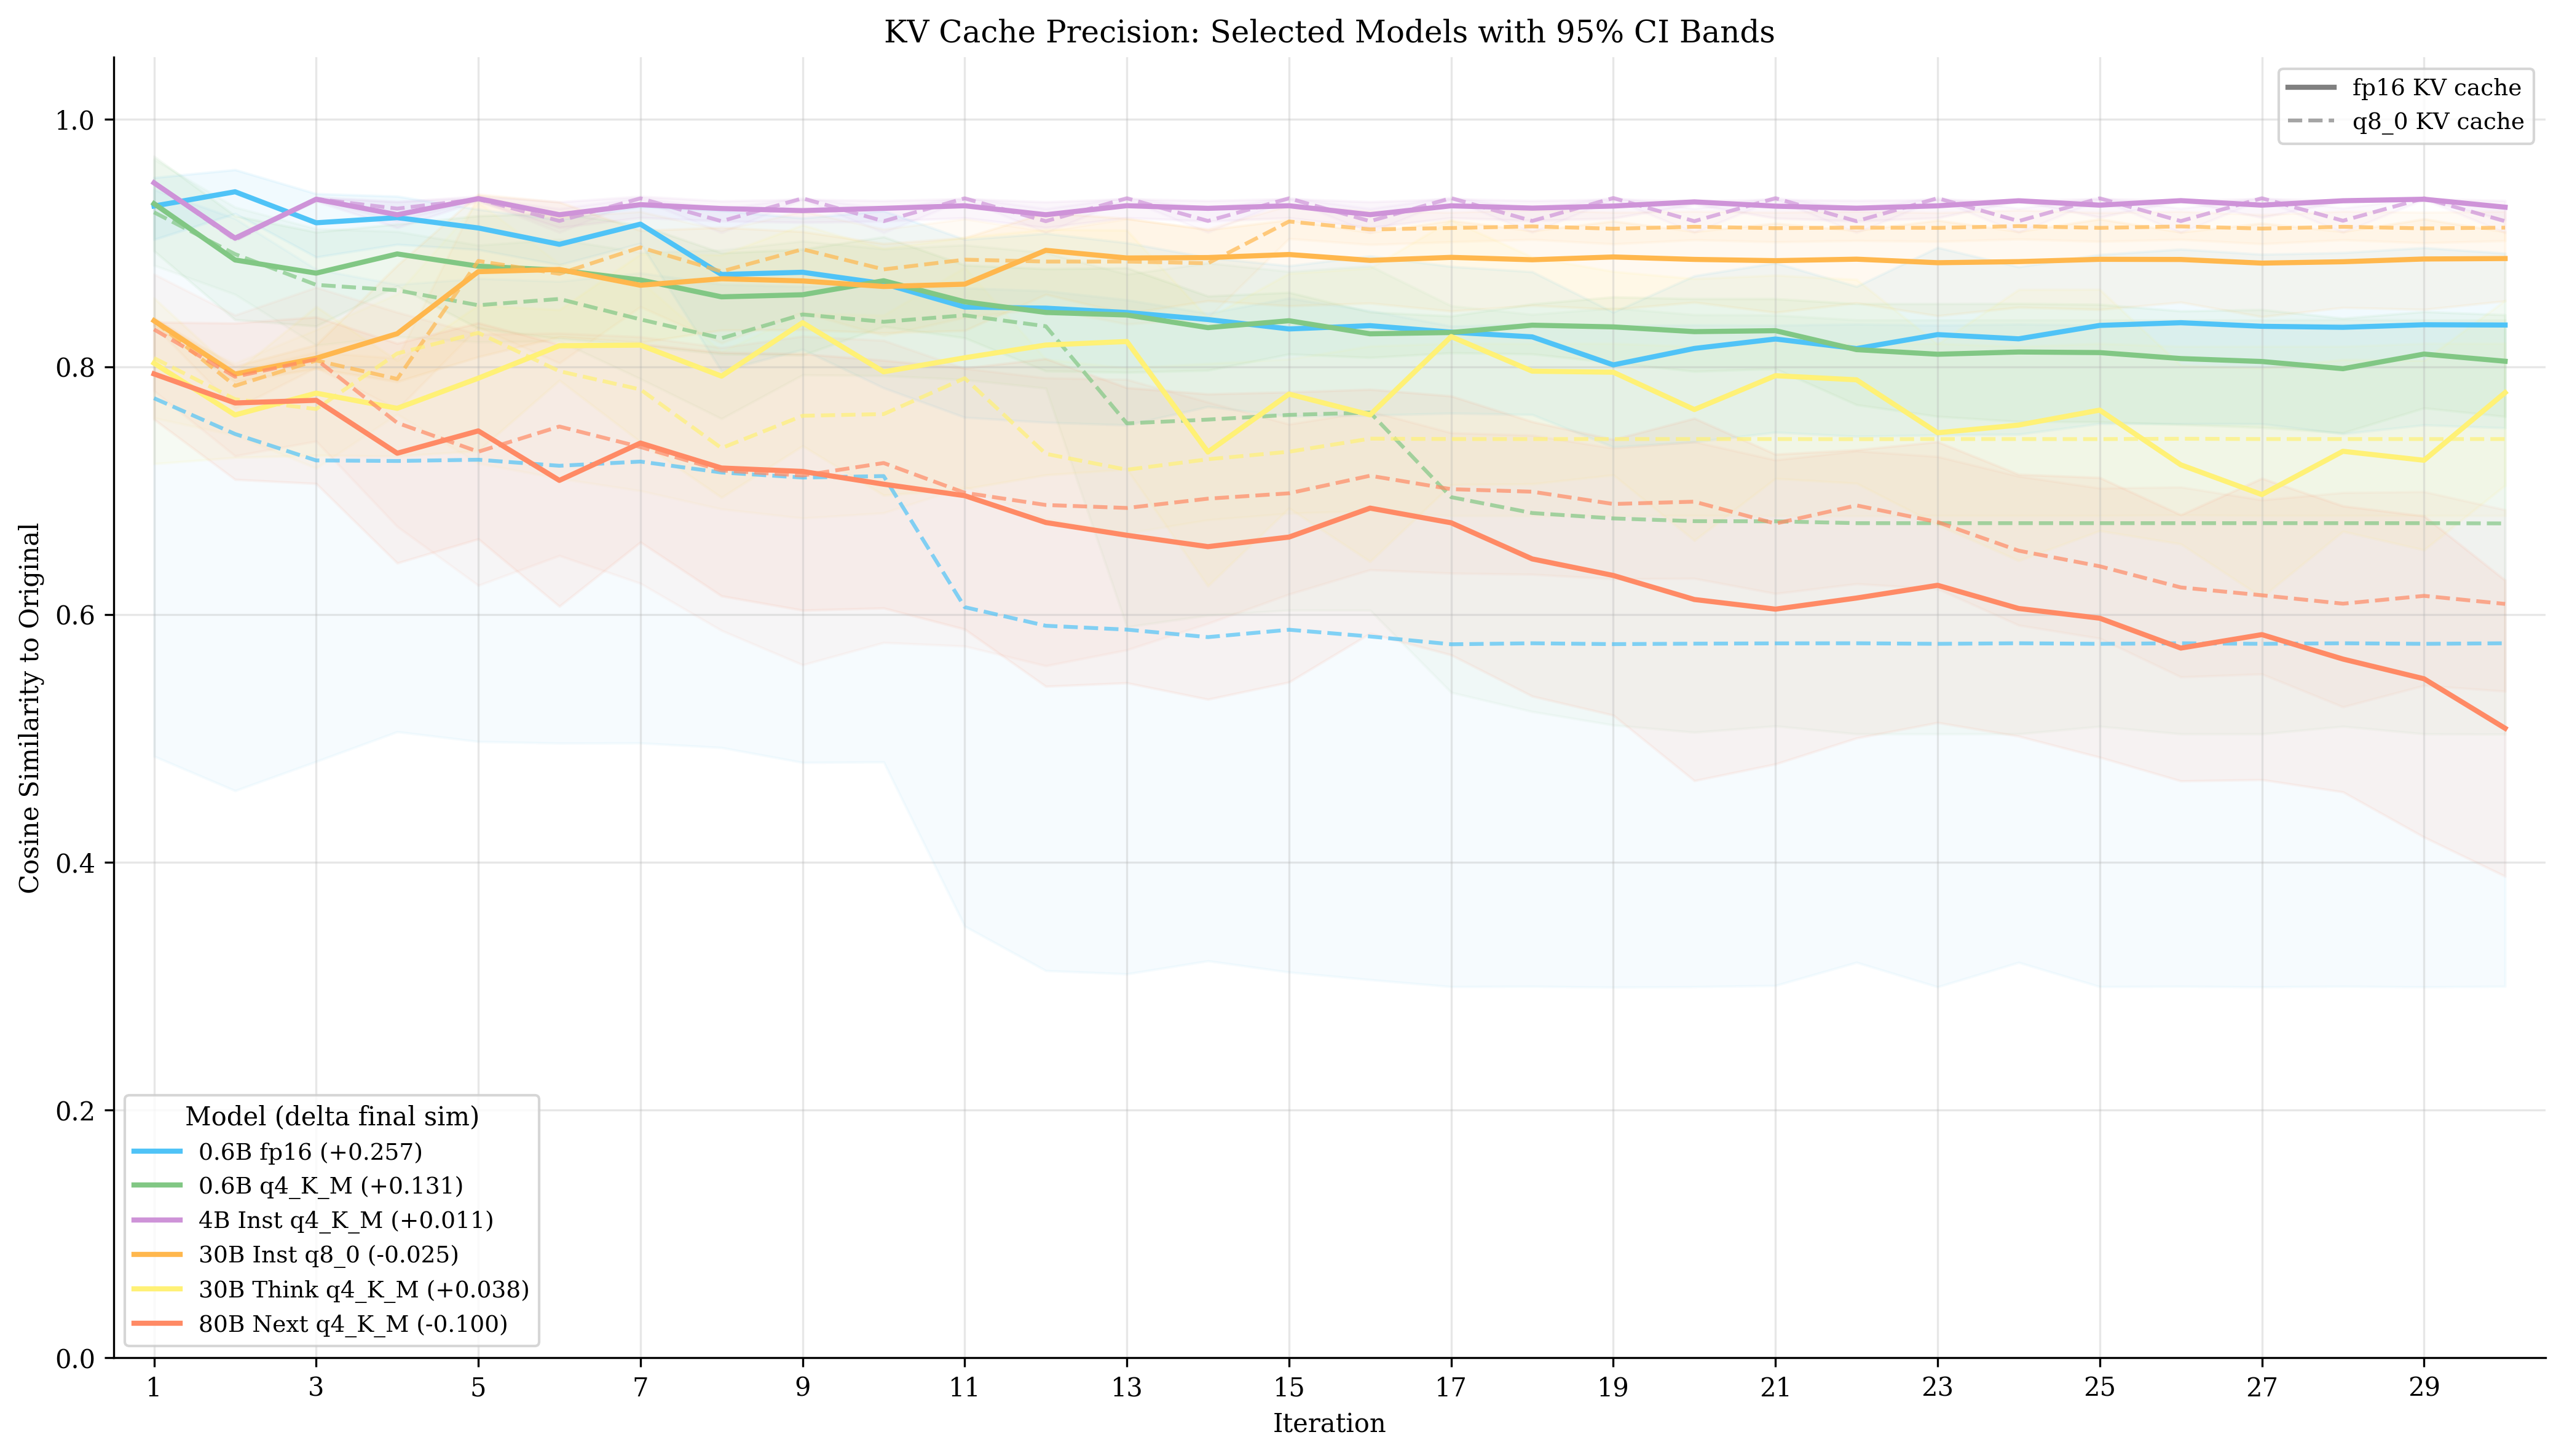
\includegraphics[width=\textwidth,height=0.31\textheight,keepaspectratio]{../results/paper_figures/figA1_rq2_overlay.png}
  \caption{KV cache precision: selected models with 95\% CI bands. Solid lines =
  fp16 KV cache; dashed = q8\_0 KV cache. 5 seeds per condition.}
  \label{fig:rq2_overlay}
\end{figure}

\begin{figure}[htbp]
  \centering
  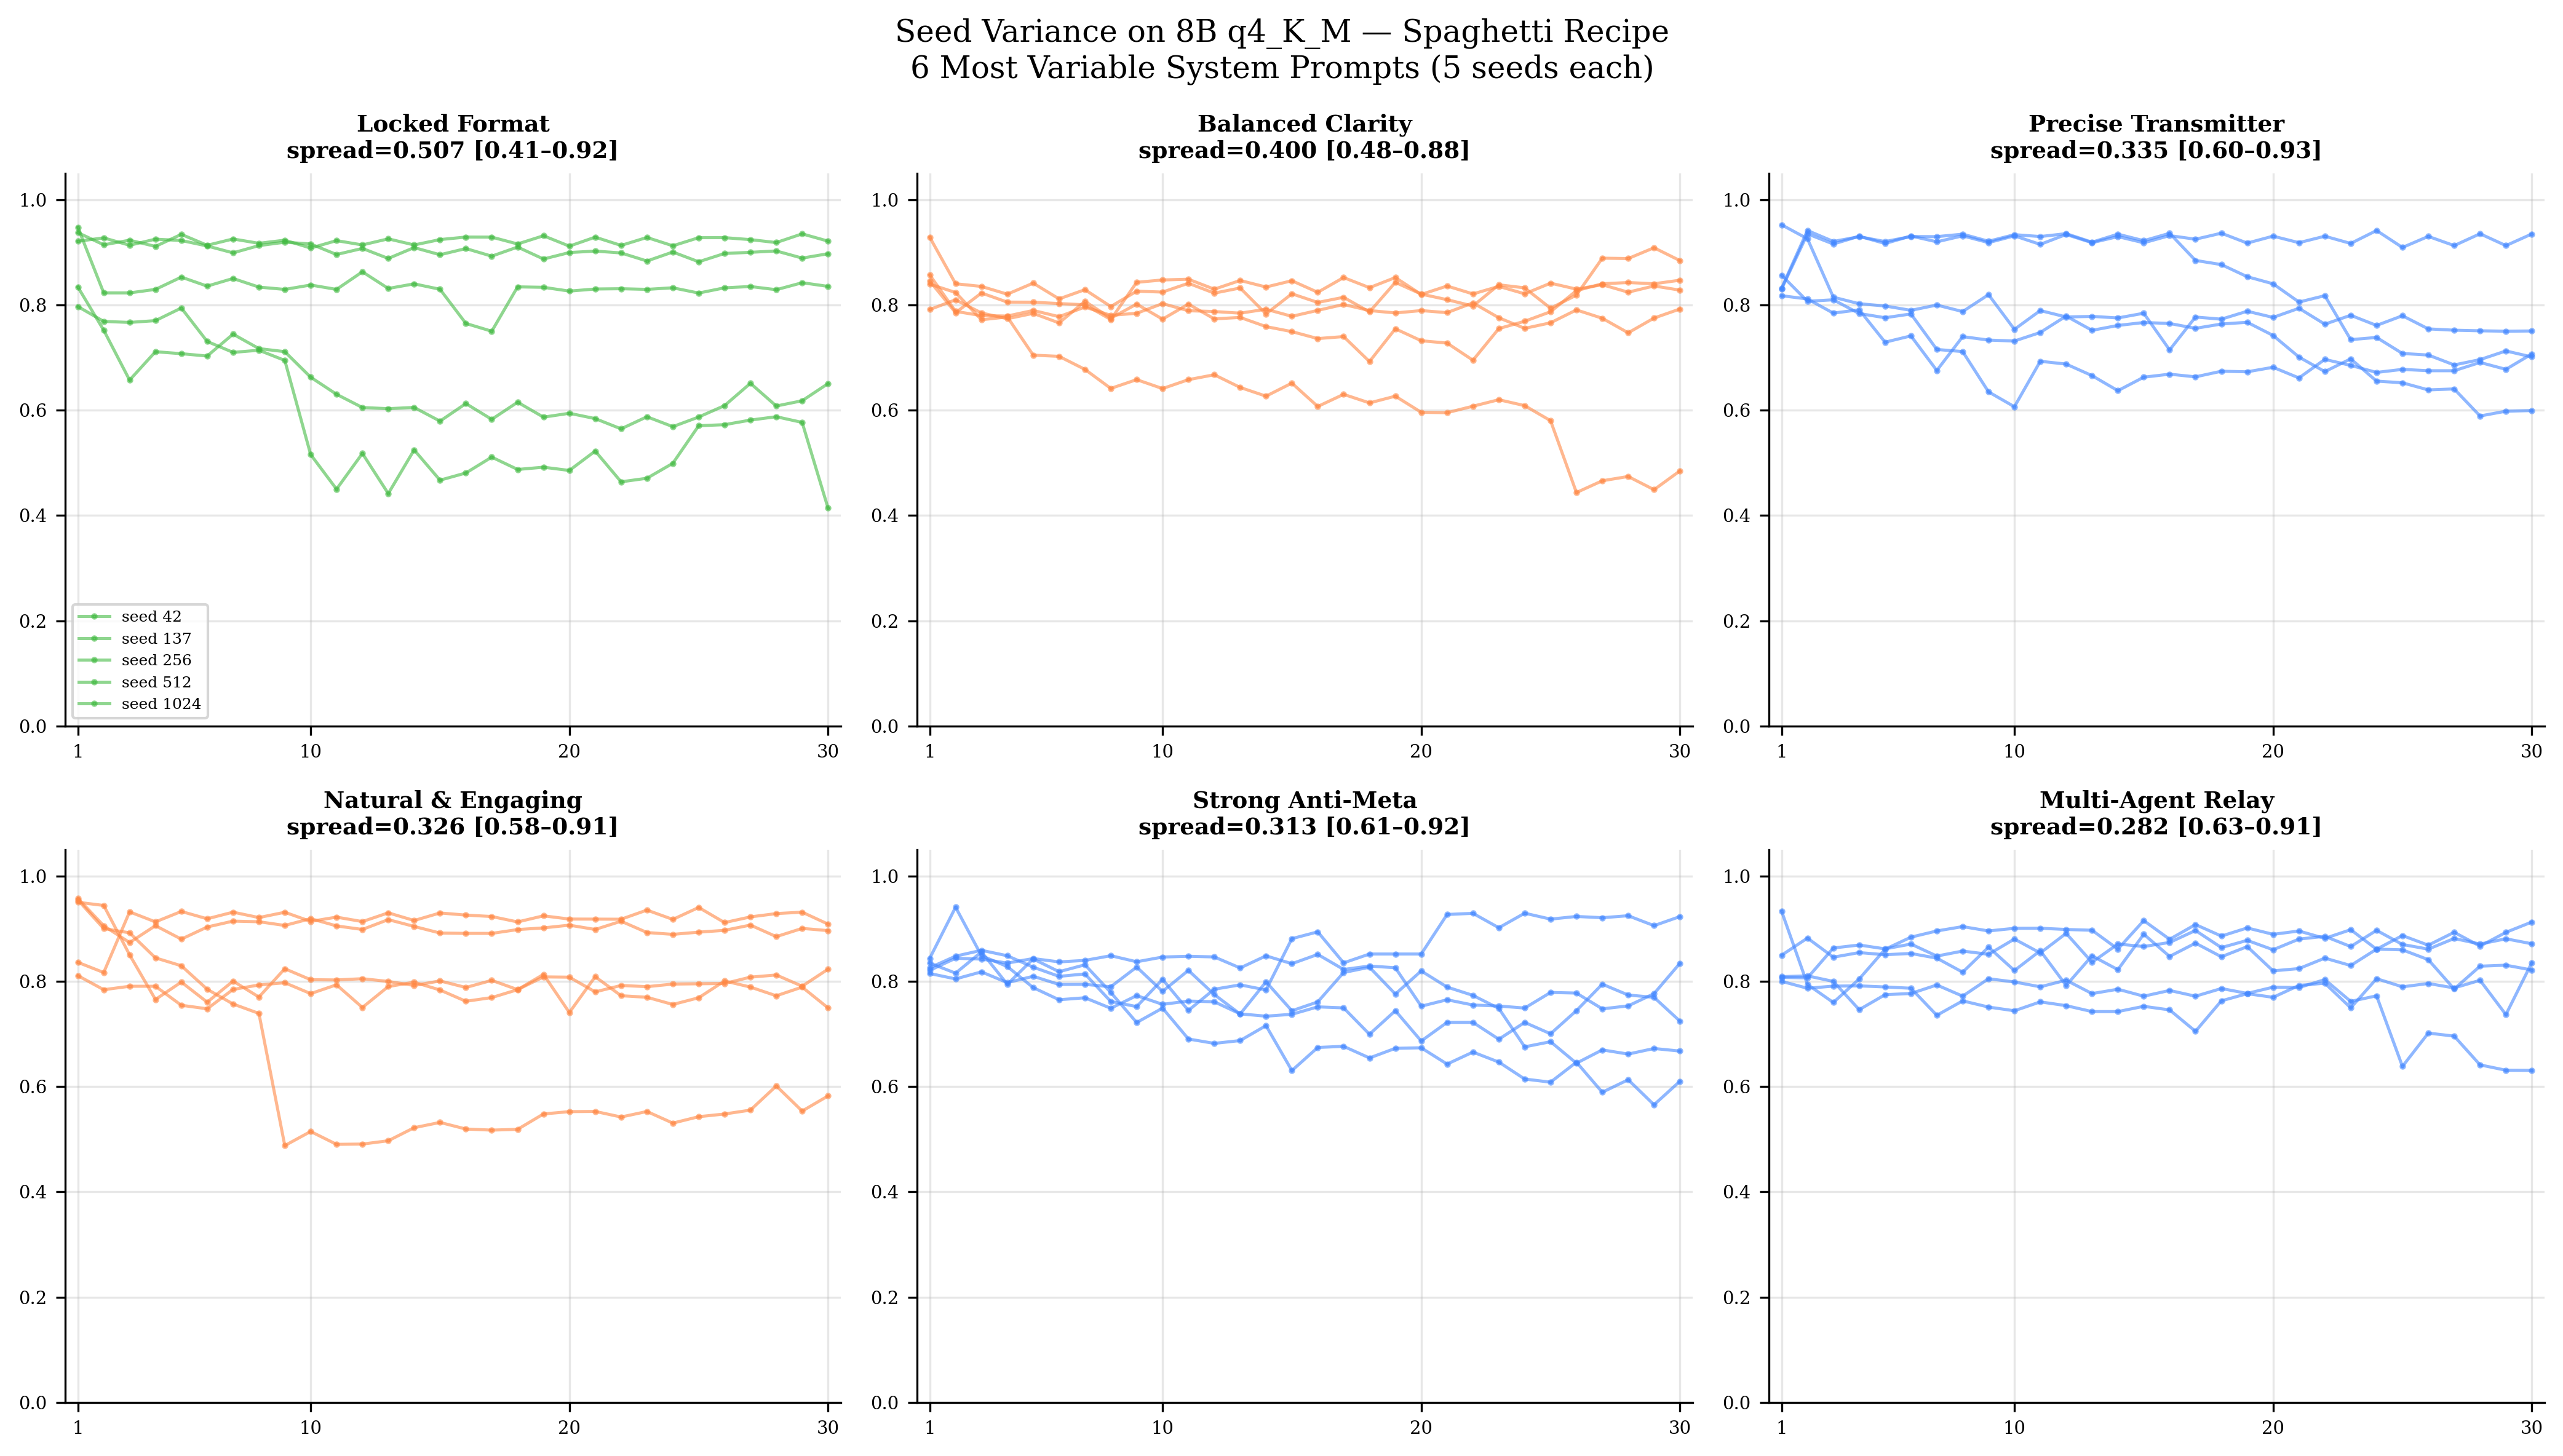
\includegraphics[width=\textwidth,height=0.31\textheight,keepaspectratio]{../results/paper_figures/figA2_seed_variance.png}
  \caption{Seed variance on 8B q4\_K\_M, spaghetti recipe. The 6 most variable
  system prompts show dramatically different trajectories across 5 seeds.}
  \label{fig:seed_variance}
\end{figure}

\begin{figure}[htbp]
  \centering
  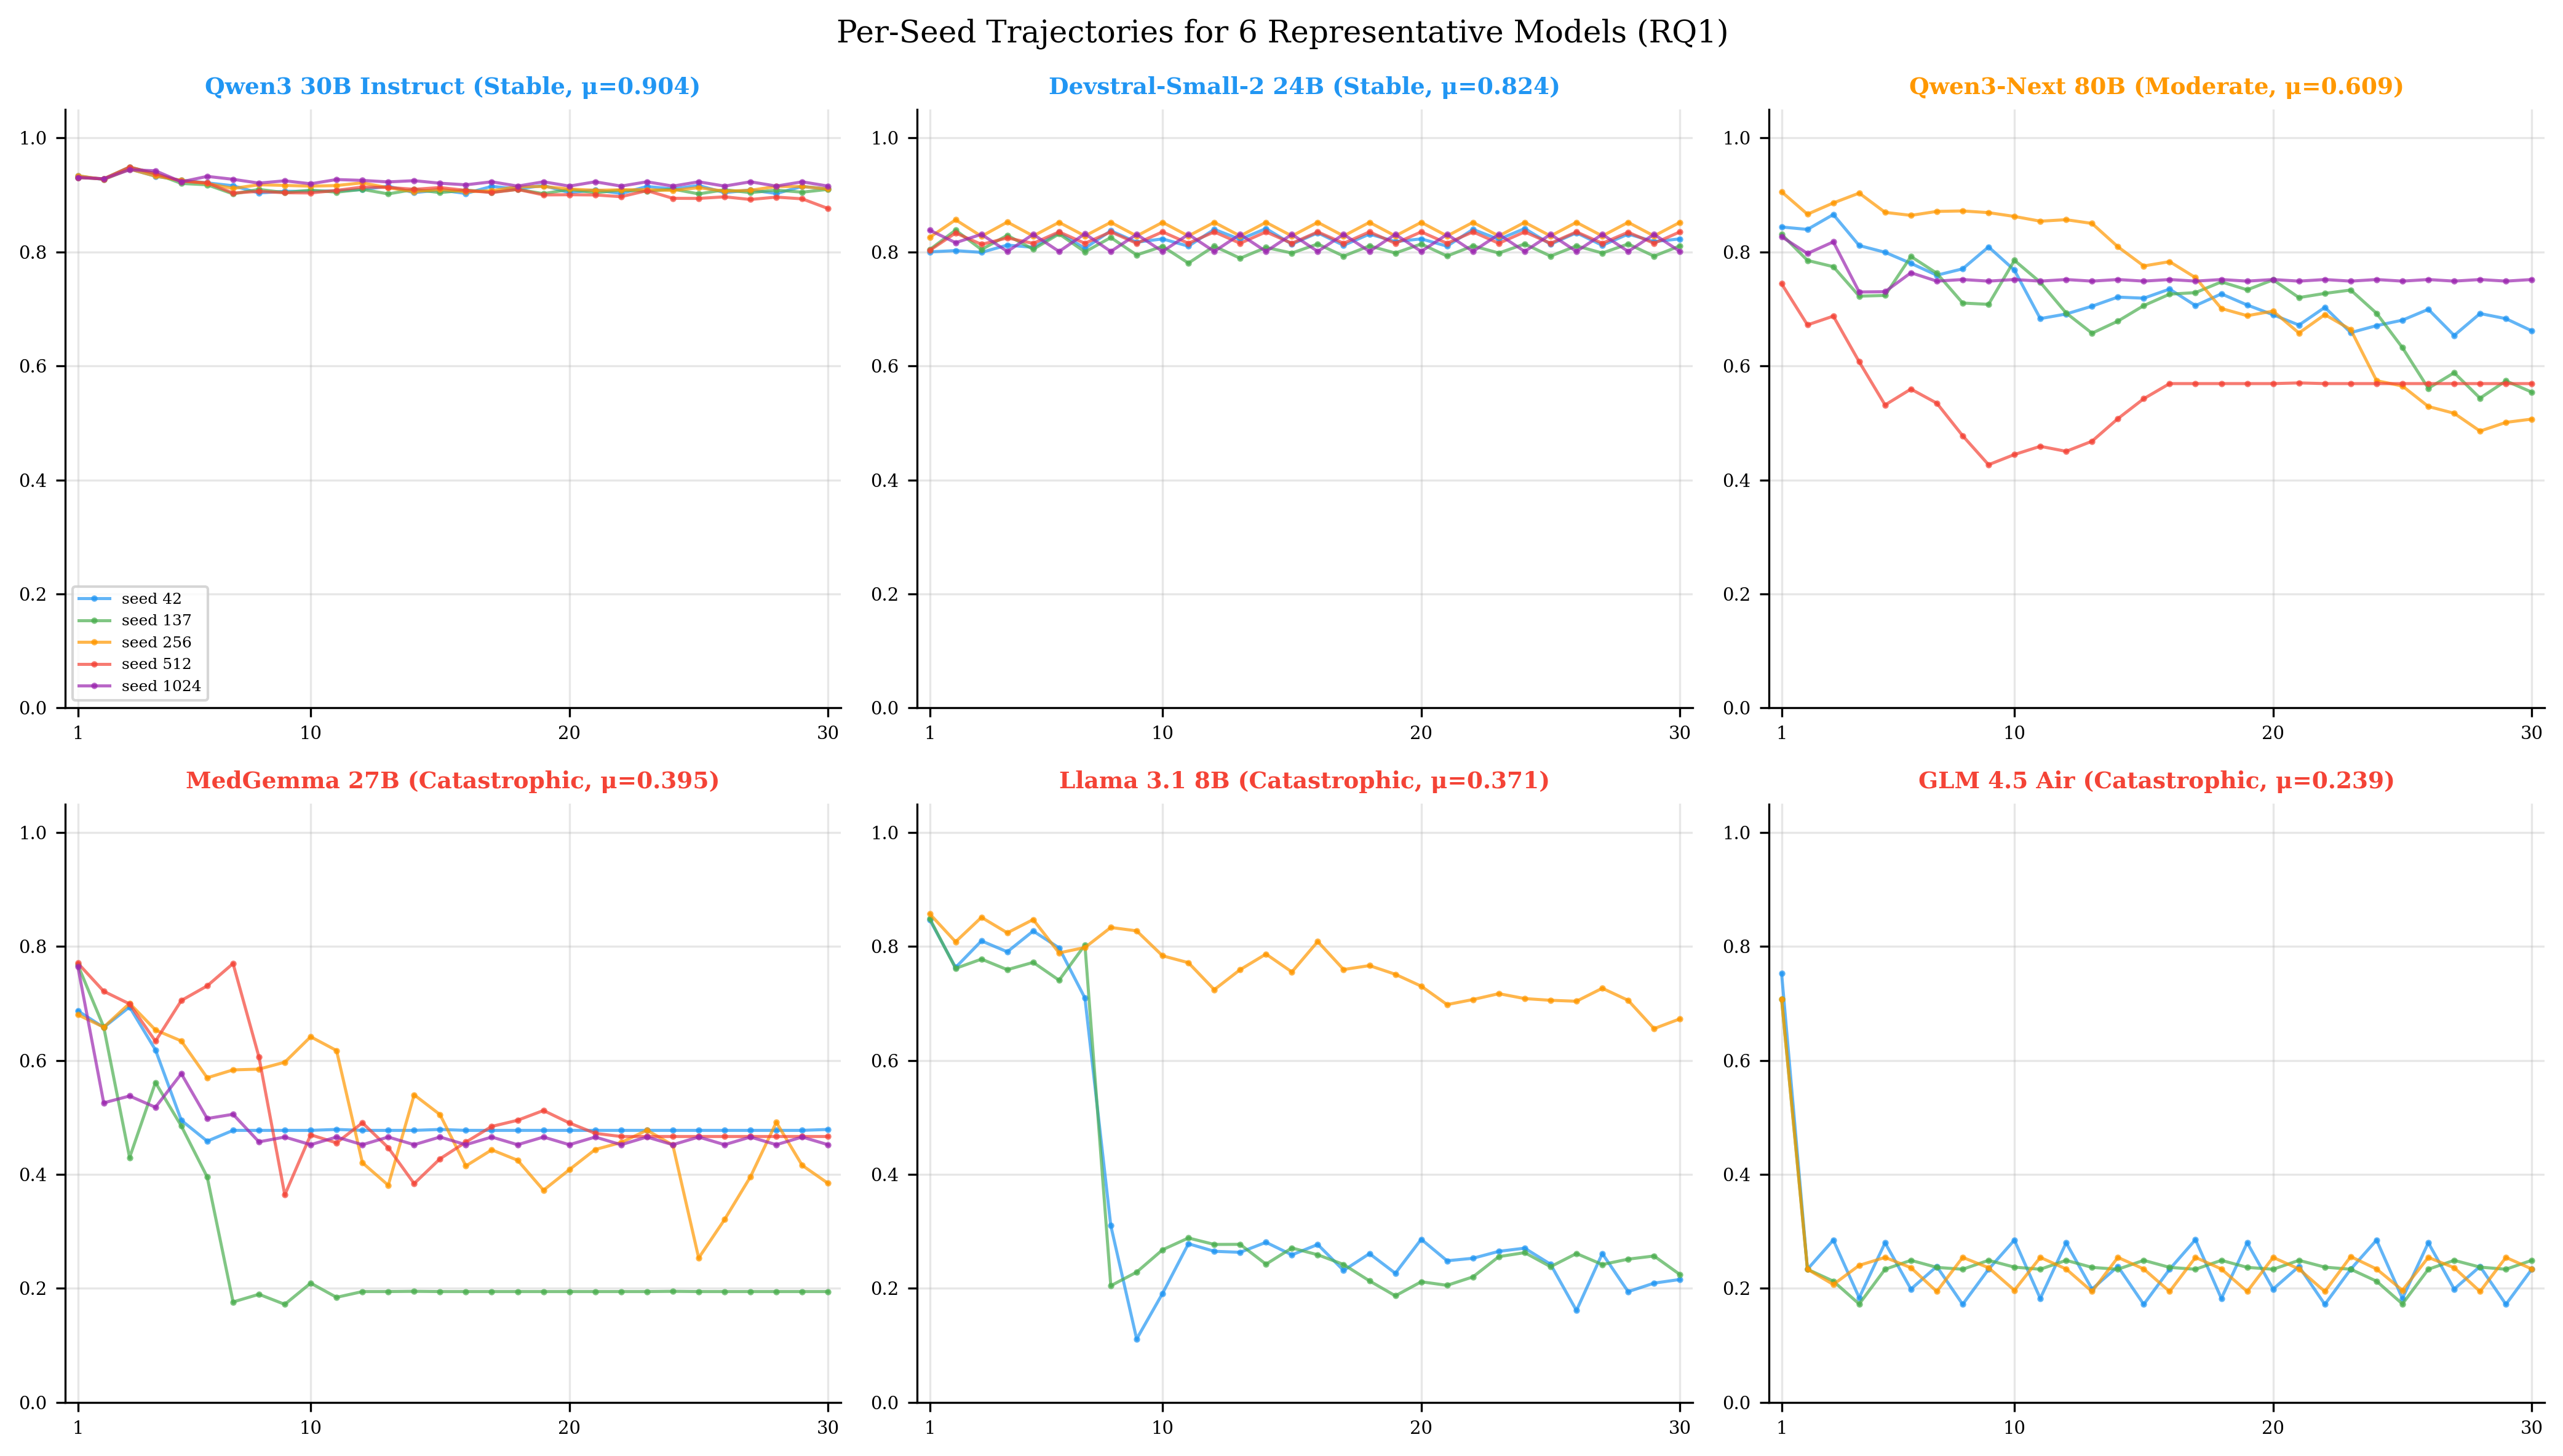
\includegraphics[width=\textwidth,height=0.31\textheight,keepaspectratio]{../results/paper_figures/figA3_rq1_small_multiples.png}
  \caption{Per-seed trajectories for 6 representative cross-family models.}
  \label{fig:rq1_small_multiples}
\end{figure}

\begin{figure}[htbp]
\centering
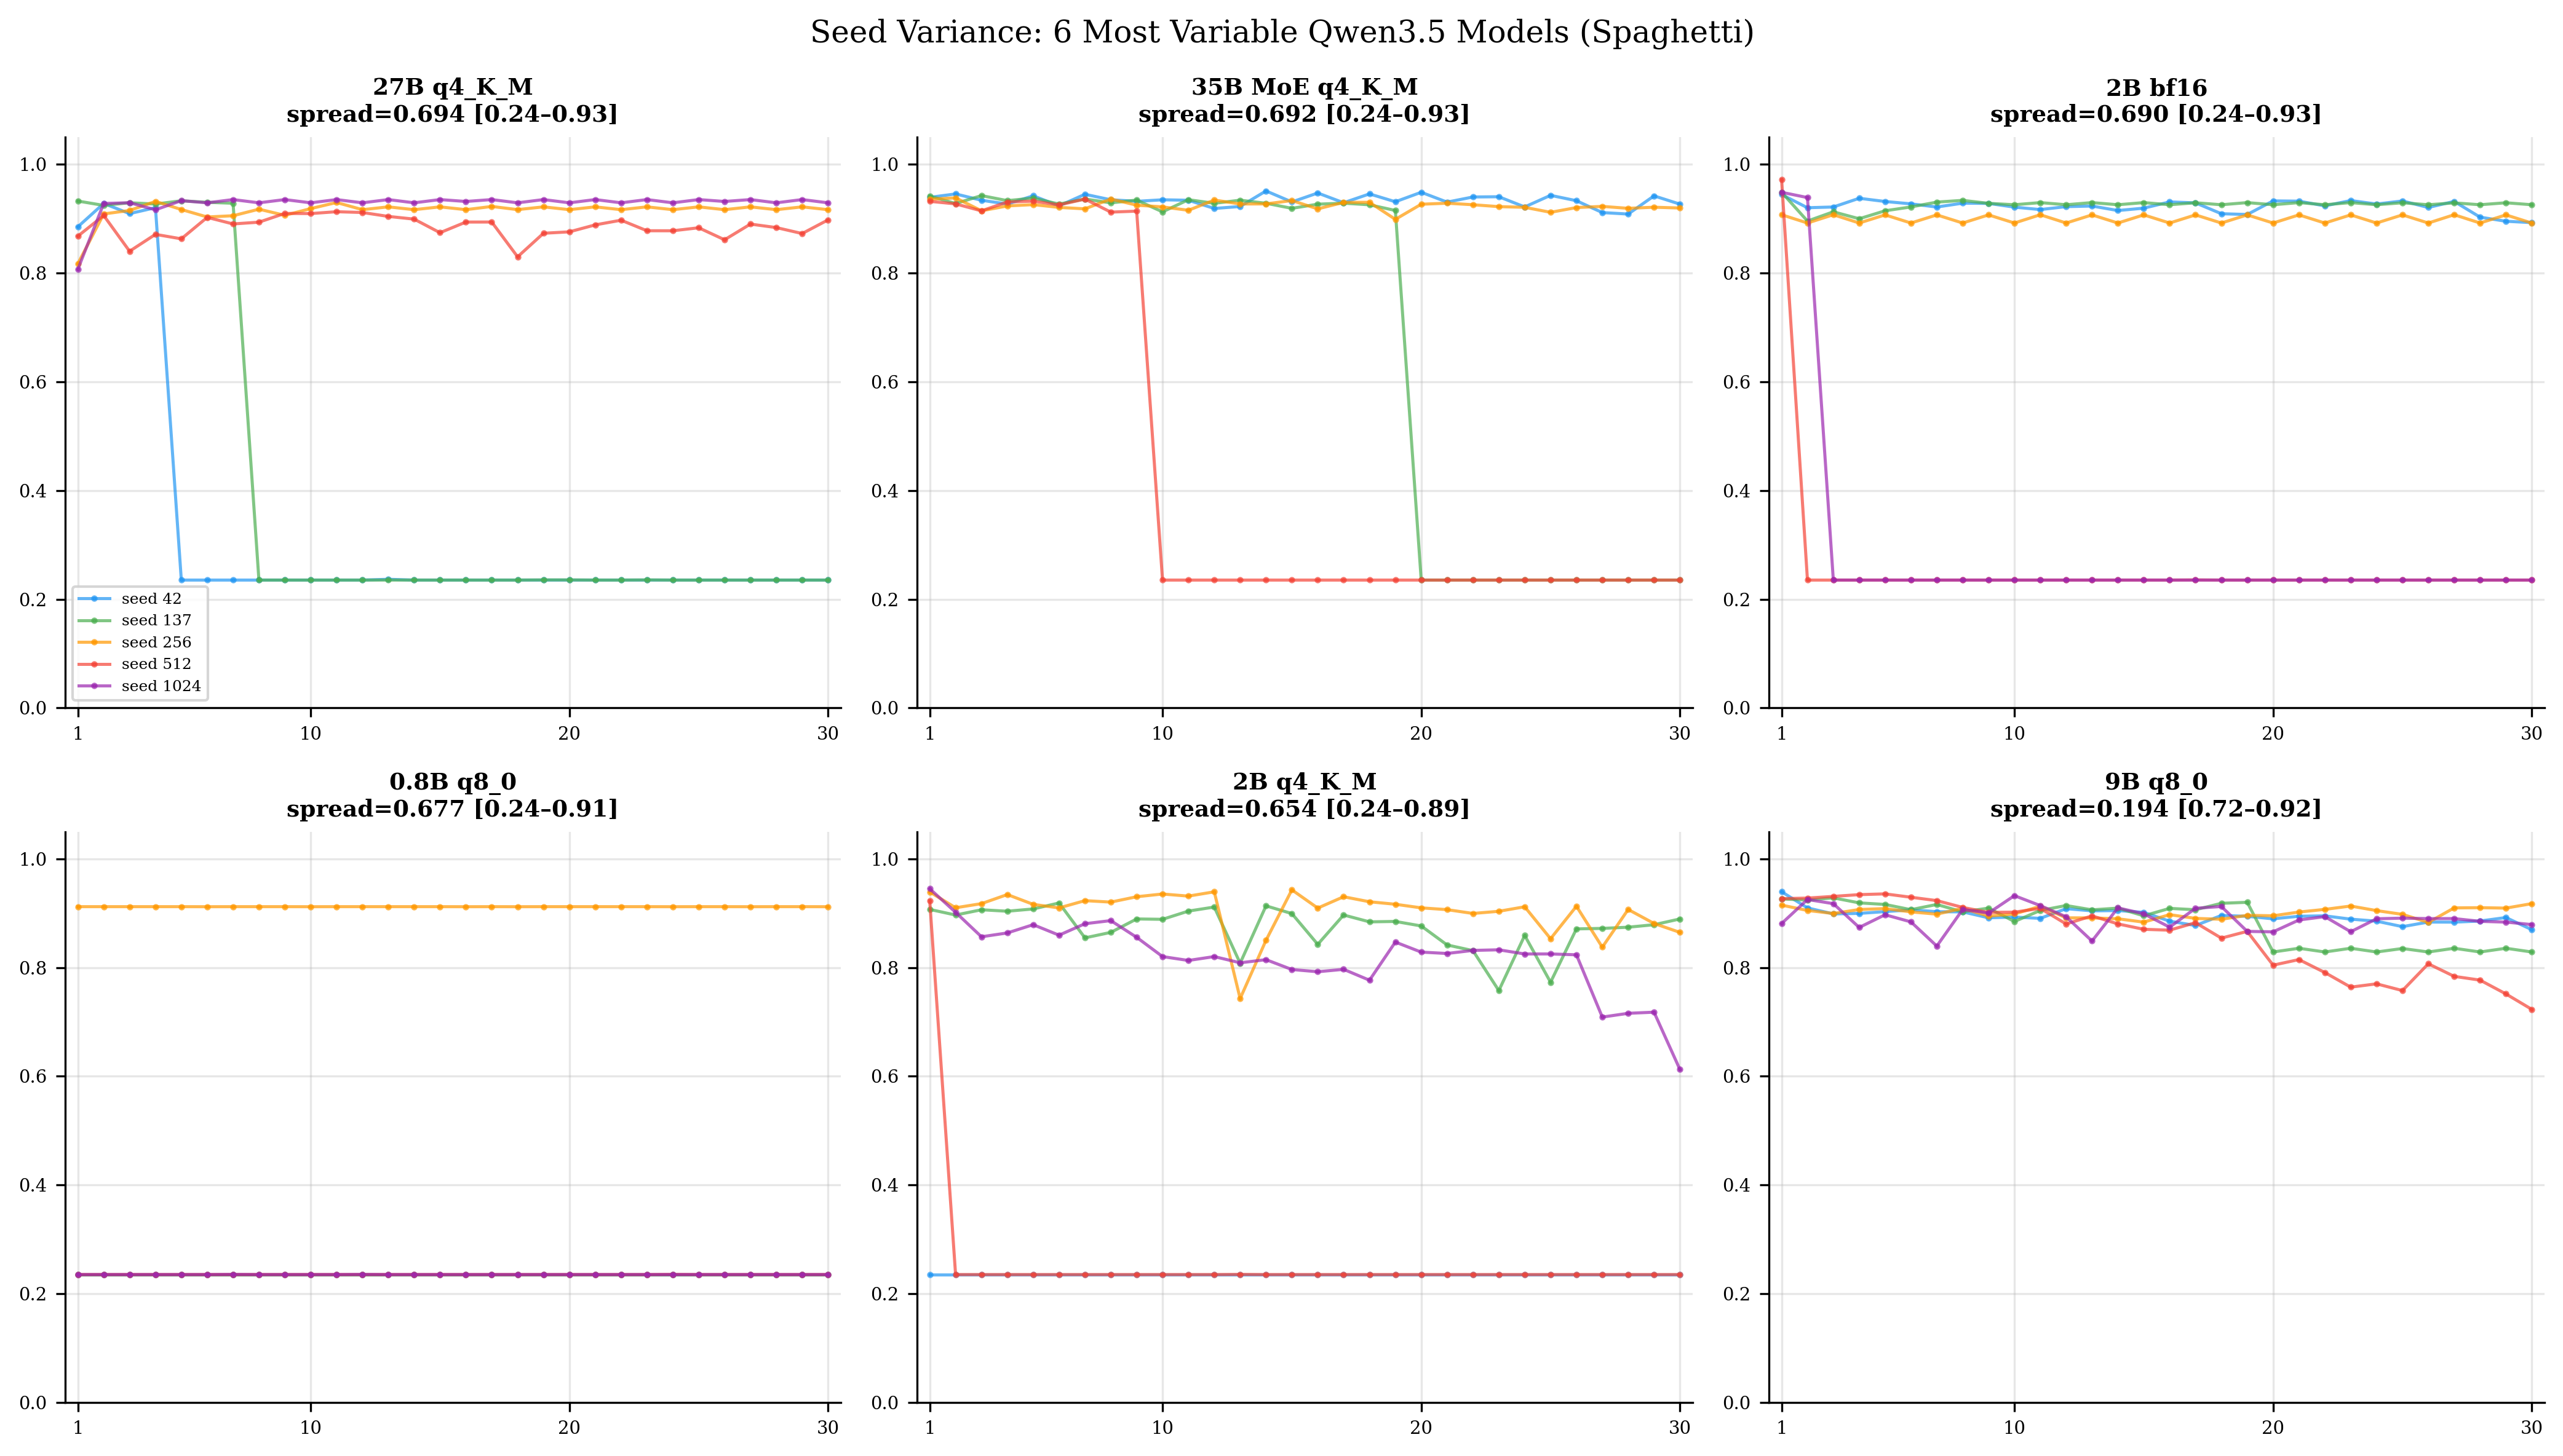
\includegraphics[width=\textwidth,height=0.31\textheight,keepaspectratio]{../results/qwen35_paper_figures/figA2_seed_variance.png}
\caption{Seed variance for the 6 most variable Qwen3.5 models on the
  spaghetti recipe. Individual seed trajectories shown.}
\label{fig:q35_seed_var}
\end{figure}

\begin{figure}[htbp]
\centering
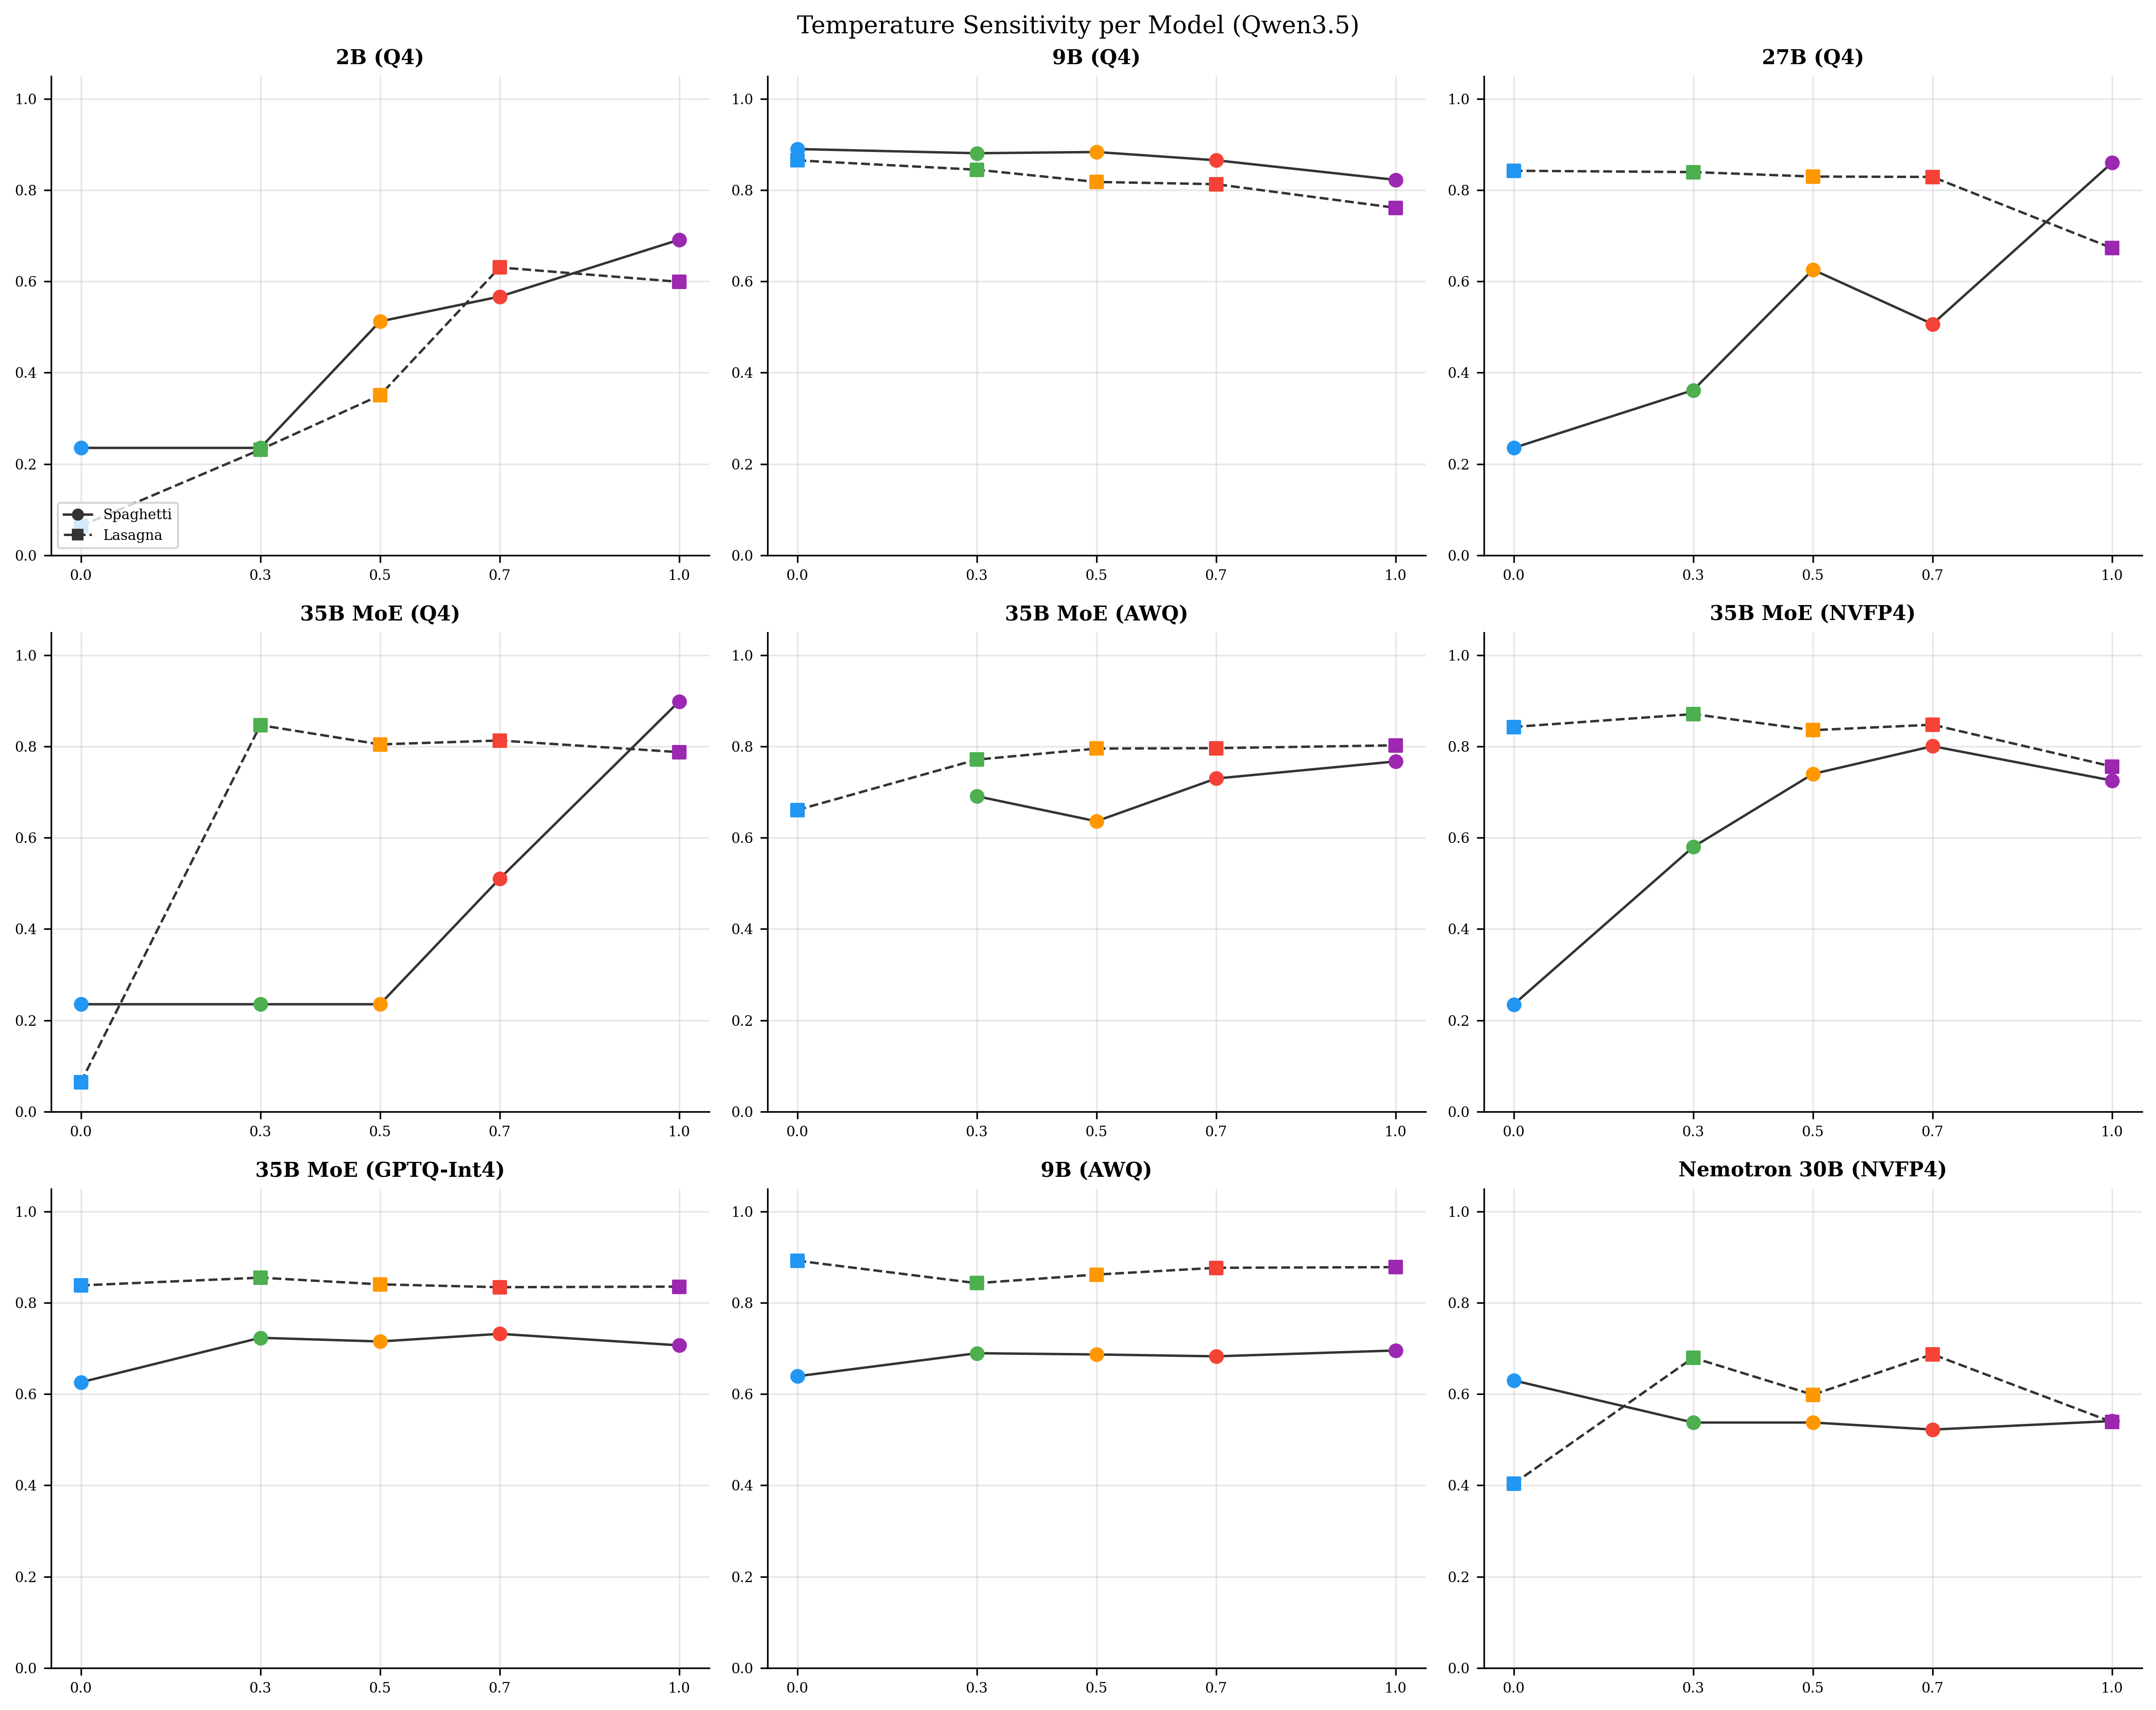
\includegraphics[width=\textwidth,height=0.31\textheight,keepaspectratio]{../results/qwen35_paper_figures/figA3_temperature_multiples.png}
\caption{Temperature sensitivity per Qwen3.5 model: mean final similarity at
  each temperature for spaghetti (solid) and lasagna (dashed).}
\label{fig:q35_temp_multi}
\end{figure}


\section{Embedding Model Validation Detail}
\label{app:embedding}

We validate the primary embedding model (Qwen3-Embedding-0.6B,
32{,}768-token context) against bge-m3 (8{,}192-token context) by re-embedding
all saved text pairs and computing Pearson and Spearman correlations between the
two models' cosine similarity scores.

On the cross-family data, all 21{,}636 pairs embedded successfully, giving
$r = 0.960$ and $\rho = 0.857$ (Figure~\ref{fig:embedding}).

On the within-family data, 20{,}072 of 22{,}167 pairs (90.6\%) produced valid
similarities from both models, yielding $r = 0.825$ and $\rho = 0.815$
($p < 10^{-10}$ for both; Figure~\ref{fig:q35_embed_val}). The remaining
2{,}095 pairs (9.4\%) failed because bge-m3's vLLM endpoint rejects inputs
exceeding its 8{,}192-token context window rather than truncating them. All
failed pairs are outputs exceeding 6{,}000 words, produced by chains that
experienced runaway text expansion---a characteristic drift failure mode in
which certain system prompts (e.g., ``Visual Tutorial Style,'' ``Friendly
Conversational'') cause outputs to grow by several thousand words over 30
iterations. These excluded pairs have a mean Qwen similarity of 0.515 (median
0.572) compared with the dataset mean of 0.829, confirming that they are
systematically the most-drifted outputs. Because both embedding models would
score these highly-diverged texts as low similarity, their exclusion is
unlikely to meaningfully affect the correlation.

\begin{figure}[htbp]
\centering
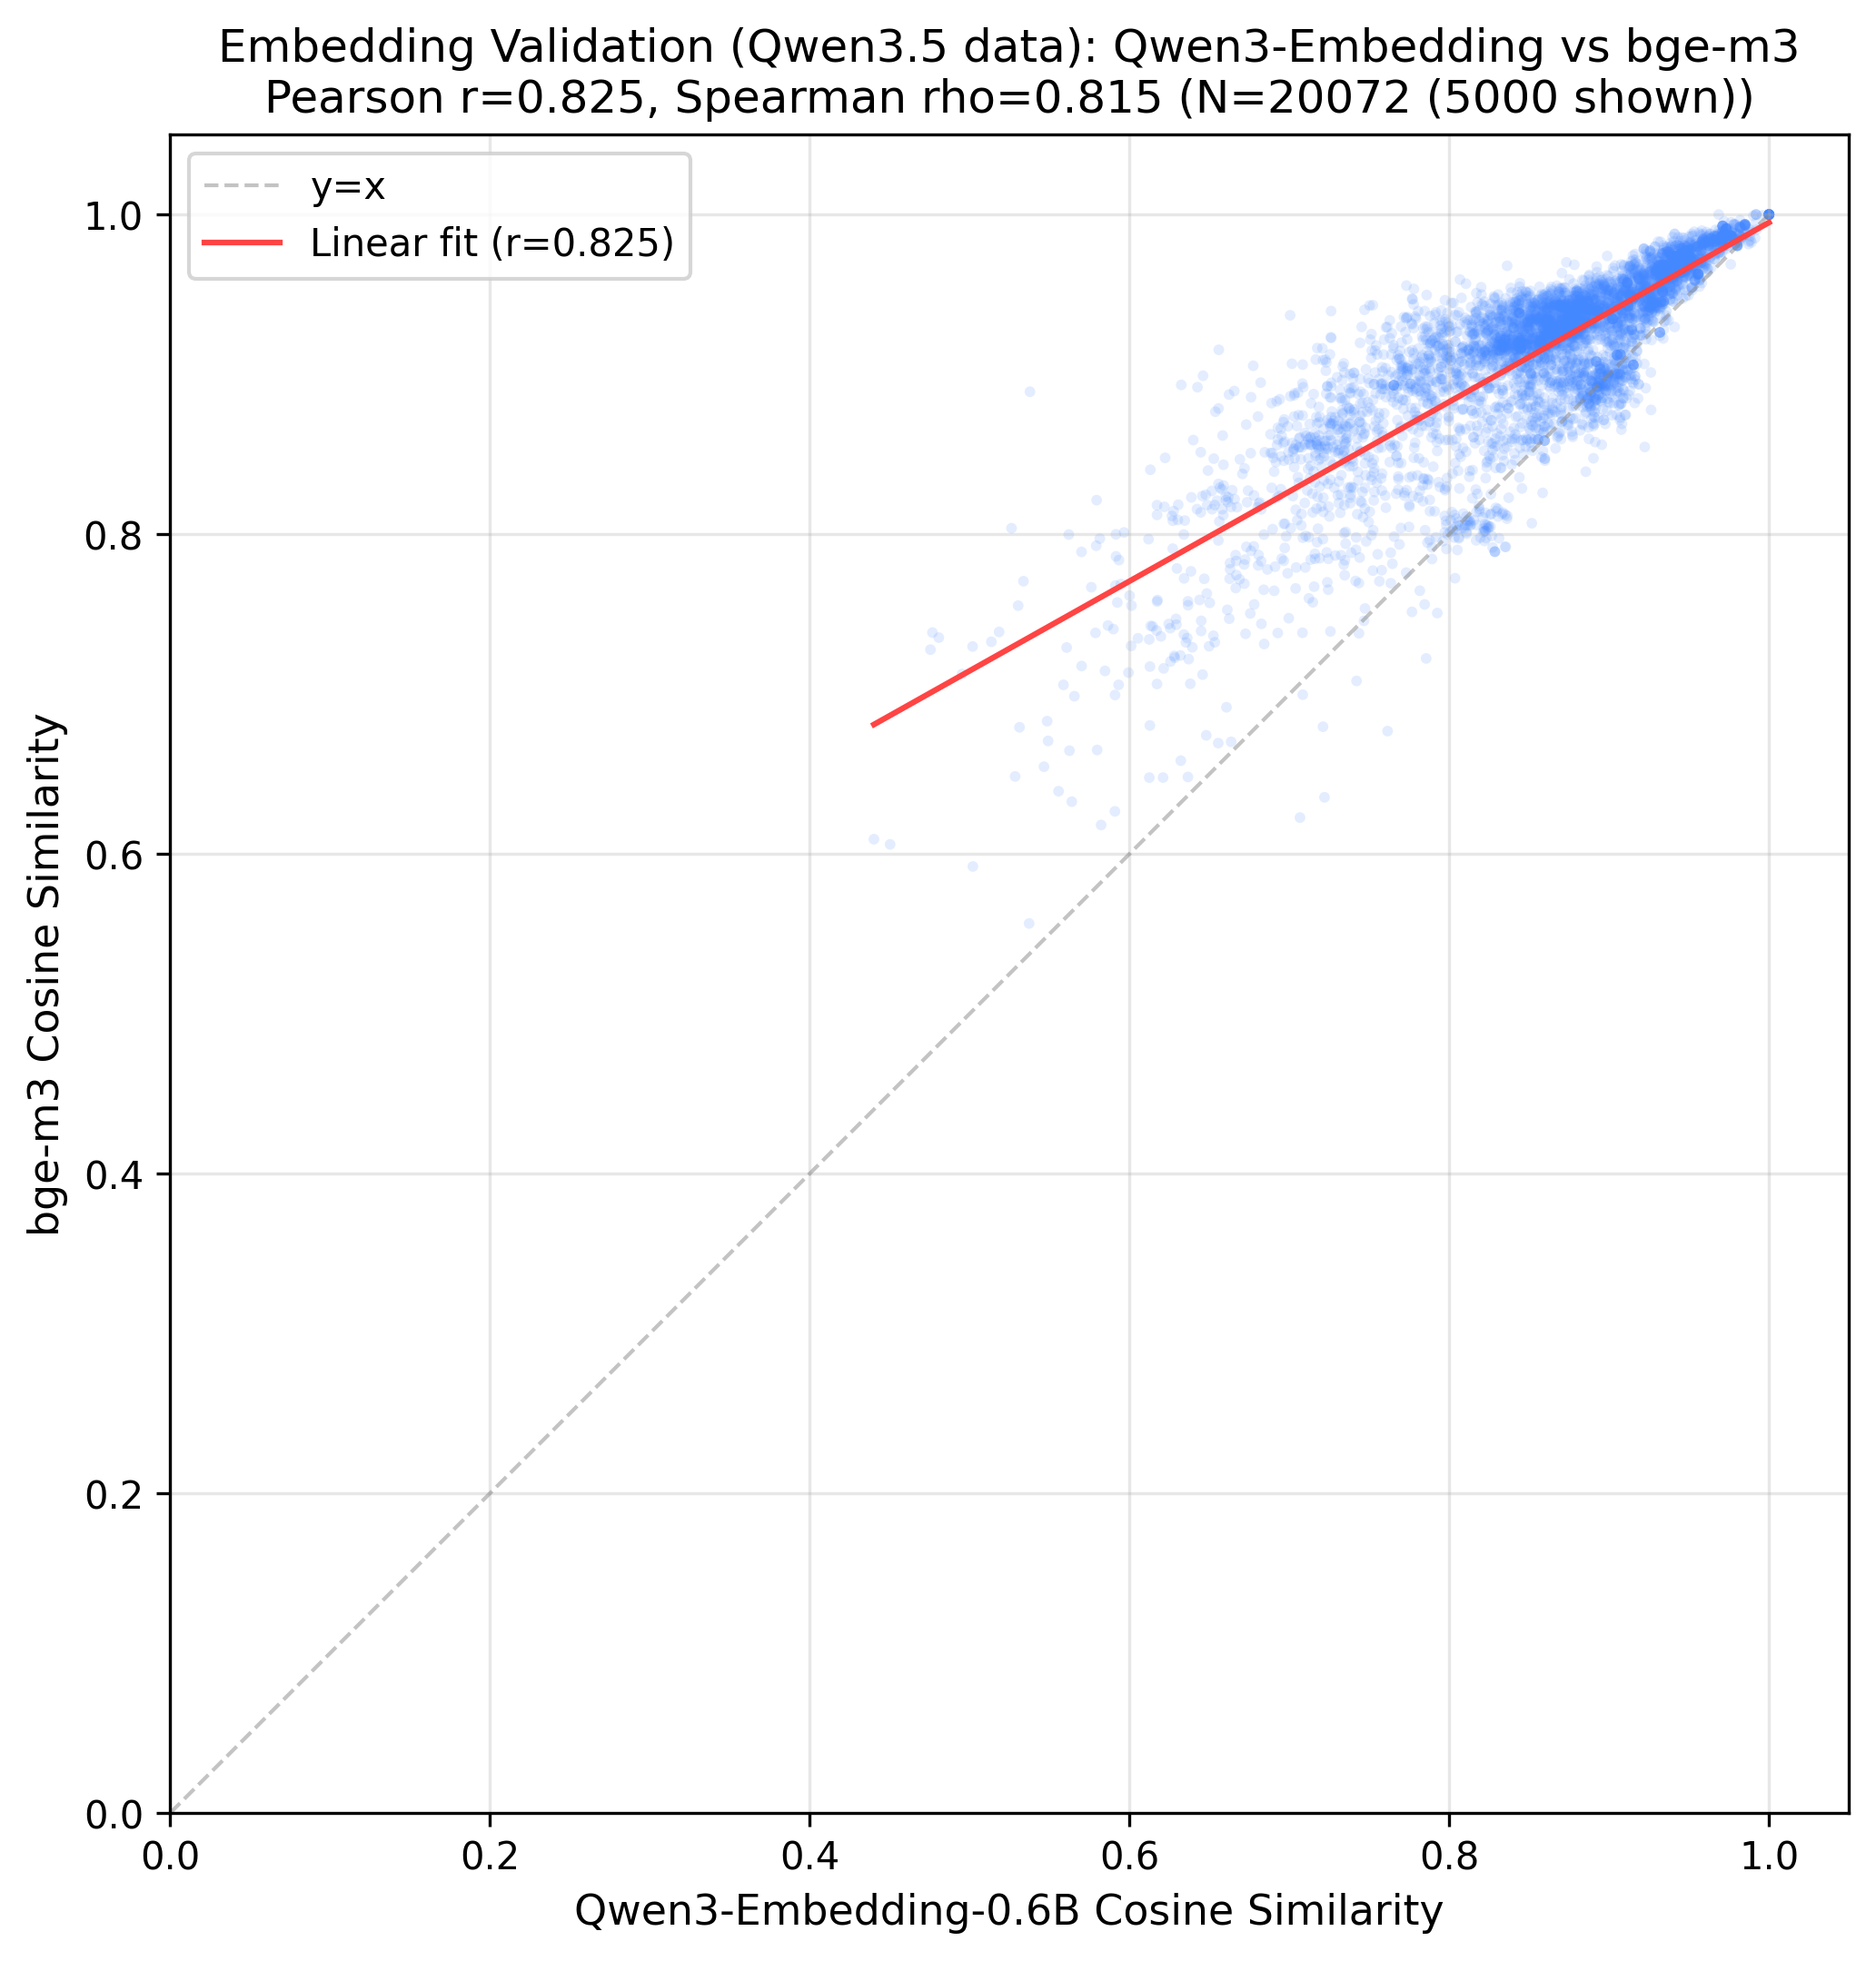
\includegraphics[width=\textwidth,height=0.31\textheight,keepaspectratio]{../results/embedding_validation_qwen35/embedding_scatter.png}
\caption{Embedding model validation scatter for the within-family data:
  Qwen3-Embedding-0.6B vs.\ bge-m3 cosine similarities for 20{,}072 Qwen3.5
  experiment text pairs (2{,}095 pairs with outputs exceeding bge-m3's
  8{,}192-token context limit excluded). Pearson $r = 0.825$,
  Spearman $\rho = 0.815$.}
\label{fig:q35_embed_val}
\end{figure}

\section{Reproducibility and Compute}
\label{app:compute}

\paragraph{Hardware.}
All Ollama and vLLM runs were executed on a single on-premises server with
one NVIDIA RTX~PRO~6000 Blackwell GPU (96\,GB). The SGLang NVFP4 runs
(35B NVFP4 and the Nemotron control) were executed on a second on-premises
server with one NVIDIA RTX~5090 GPU (32\,GB). Embeddings were computed with
Qwen3-Embedding-0.6B served by vLLM on a dedicated NVIDIA RTX~5070~Ti GPU
(16\,GB). The validation embeddings used bge-m3: for the cross-family dataset
served by Ollama on the RTX~PRO~6000, and for the within-family dataset served
by vLLM on an RTX~5070~Ti.

\paragraph{Software.}
Ollama v0.16.3; vLLM v0.15.1, plus a CUDA~13.0 nightly build of vLLM for the
GPTQ-Int4 and 9B~AWQ runs; SGLang for the NVFP4 runs. Analysis used Python
with NumPy, SciPy and Matplotlib, driven by
\texttt{scripts/\allowbreak analyze\_paper.py} and
\texttt{scripts/\allowbreak analyze\_qwen35\_paper.py}, which regenerate every
figure, table and reported statistic in this paper from the raw per-iteration
records; dependencies are pinned with \texttt{uv}.

\paragraph{Scale and compute budget.}
The cross-family experiments comprise 669 seeded chains and 20{,}070 attempted
inferences, of which 19{,}798 returned a scored output; 658 chains ran the full
30 iterations. Summing the recorded per-iteration wall-clock times across those
data files gives approximately 61 hours of cumulative inference time. The
within-family experiments comprise 1{,}969 completed 30-iteration chains, that
is 59{,}070 inferences, drawn from 2{,}007 launched chains; summing their
recorded per-iteration times gives approximately 630 hours of cumulative
inference time. Because several of those experiments ran with up to four
concurrent workers, the elapsed wall-clock duration of the campaign was
substantially shorter than that figure. Embedding validation added 21{,}636 and
22{,}167 further embedding pairs respectively.

\paragraph{Availability.}
The experiment scripts, the analysis code that produces every figure and
table in this paper, and the raw per-iteration drift records (every chain's
input and output text) are available at
\url{https://github.com/jhsmith409/telephone-semantic-drift}; the drift
records are attached to the repository's \texttt{v1.0-data} release as a
compressed archive with a published SHA-256 checksum.

\end{document}
